% Options for packages loaded elsewhere
\PassOptionsToPackage{unicode}{hyperref}
\PassOptionsToPackage{hyphens}{url}
%
\documentclass[
  11pt,
  twoside]{article}
\usepackage{amsmath,amssymb}
\usepackage{setspace}
\usepackage{iftex}
\ifPDFTeX
  \usepackage[T1]{fontenc}
  \usepackage[utf8]{inputenc}
  \usepackage{textcomp} % provide euro and other symbols
\else % if luatex or xetex
  \usepackage{unicode-math} % this also loads fontspec
  \defaultfontfeatures{Scale=MatchLowercase}
  \defaultfontfeatures[\rmfamily]{Ligatures=TeX,Scale=1}
\fi
\usepackage{lmodern}
\ifPDFTeX\else
  % xetex/luatex font selection
  \setmainfont[]{DejaVu Serif}
\fi
% Use upquote if available, for straight quotes in verbatim environments
\IfFileExists{upquote.sty}{\usepackage{upquote}}{}
\IfFileExists{microtype.sty}{% use microtype if available
  \usepackage[]{microtype}
  \UseMicrotypeSet[protrusion]{basicmath} % disable protrusion for tt fonts
}{}
\makeatletter
\@ifundefined{KOMAClassName}{% if non-KOMA class
  \IfFileExists{parskip.sty}{%
    \usepackage{parskip}
  }{% else
    \setlength{\parindent}{0pt}
    \setlength{\parskip}{6pt plus 2pt minus 1pt}}
}{% if KOMA class
  \KOMAoptions{parskip=half}}
\makeatother
\usepackage{xcolor}
\usepackage[paperwidth=6.14in,paperheight=9.21in,inner=0.75in,outer=0.65in,top=0.68in,bottom=0.72in,includeheadfoot,headheight=14pt]{geometry}
\usepackage{longtable,booktabs,array}
\usepackage{calc} % for calculating minipage widths
% Correct order of tables after \paragraph or \subparagraph
\usepackage{etoolbox}
\makeatletter
\patchcmd\longtable{\par}{\if@noskipsec\mbox{}\fi\par}{}{}
\makeatother
% Allow footnotes in longtable head/foot
\IfFileExists{footnotehyper.sty}{\usepackage{footnotehyper}}{\usepackage{footnote}}
\makesavenoteenv{longtable}
\usepackage{graphicx}
\makeatletter
\def\maxwidth{\ifdim\Gin@nat@width>\linewidth\linewidth\else\Gin@nat@width\fi}
\def\maxheight{\ifdim\Gin@nat@height>\textheight\textheight\else\Gin@nat@height\fi}
\makeatother
% Scale images if necessary, so that they will not overflow the page
% margins by default, and it is still possible to overwrite the defaults
% using explicit options in \includegraphics[width, height, ...]{}
\setkeys{Gin}{width=\maxwidth,height=\maxheight,keepaspectratio}
% Set default figure placement to htbp
\makeatletter
\def\fps@figure{htbp}
\makeatother
\setlength{\emergencystretch}{3em} % prevent overfull lines
\providecommand{\tightlist}{%
  \setlength{\itemsep}{0pt}\setlength{\parskip}{0pt}}
\setcounter{secnumdepth}{5}
\ifLuaTeX
\usepackage[bidi=basic]{babel}
\else
\usepackage[bidi=default]{babel}
\fi
\babelprovide[main,import]{american}
\ifPDFTeX
\else
\babelfont{rm}[]{DejaVu Serif}
\fi
% get rid of language-specific shorthands (see #6817):
\let\LanguageShortHands\languageshorthands
\def\languageshorthands#1{}
\usepackage{microtype}
\usepackage{xurl}
\usepackage{tocloft}
\AtBeginDocument{\let\ArcSecsTOC\tableofcontents\renewcommand{\tableofcontents}{\begingroup\small\ArcSecsTOC\endgroup}}
\setlength{\cftsecnumwidth}{2.5em}
\setlength{\cftbeforesecskip}{2pt}
\setlength{\cftsubsecindent}{2.5em}
\setlength{\cftsubsecnumwidth}{3.1em}
\usepackage{float}
\floatplacement{figure}{H}
\setlength{\emergencystretch}{3em}
\setlength{\tabcolsep}{3pt}
\setlength{\parindent}{0pt}
\setlength{\parskip}{4pt}
\raggedbottom
\usepackage{fancyhdr}
\pagestyle{fancy}
\fancyhf{}
\fancyhead[LE,RO]{\small ArcSecs | Review 6.0}
\fancyfoot[LE,RO]{\thepage}
\renewcommand{\headrulewidth}{0.3pt}
\ifLuaTeX
  \usepackage{selnolig}  % disable illegal ligatures
\fi
\usepackage{bookmark}
\IfFileExists{xurl.sty}{\usepackage{xurl}}{} % add URL line breaks if available
\urlstyle{same}
\hypersetup{
  pdftitle={ArcSecs: A Physical-Process Research Program for Photon Propagation, Cosmic Distance, and Relational Inertia},
  pdflang={en-US},
  hidelinks,
  pdfcreator={LaTeX via pandoc}}

\title{ArcSecs: A Physical-Process Research Program for Photon
Propagation, Cosmic Distance, and Relational Inertia}
\usepackage{etoolbox}
\makeatletter
\providecommand{\subtitle}[1]{% add subtitle to \maketitle
  \apptocmd{\@title}{\par {\large #1 \par}}{}{}
}
\makeatother
\subtitle{Scientific Review 6.0 --- Forward-coherent conversion and
integrated research manuscript for BEYOND SPACETIME}
\author{}
\date{24 November 2026 \textbar{} Review edition 6.0}

\begin{document}
\maketitle

{
\setcounter{tocdepth}{2}
\tableofcontents
}
\setstretch{1.06}
\newpage

\section{Abstract}\label{abstract}

ArcSecs investigates physical mechanisms for photon propagation, matter
motion, gravity, clocks and cosmic distance under twelve stipulated
foundations. C-01 asks why newly emitted light starts at its local
ceiling and then slows. Review 6.0 retains earlier results,
independently audited corrections and the static-wall continuous
interval certificate. Exact finite-energy emission at the common
characteristic remains open. Part XXXIV derives a finite-range exchange
kernel and its nonzero inelastic momentum-transfer floor. Even the
formal long-range limit strongly scatters the reference conversion. A
distinct phase-matched collective reservoir permits collinear
energy-conserving conversion into a slower positive-gap branch. Finite
reciprocal cells reveal back-conversion and frequency selectivity; an
outgoing-reservoir escape model yields a continuous monotonicity
condition for total converted population, not individual photon speed.
All are conditional mathematical or numerical results, not experimental
measurements. The earlier scalar bath, reduced history, and local vector
candidates remain distinct. No common parameter set or calibrated
astronomical fit has fulfilled the full charter.

\textbf{Keywords:} ArcSecs; C-01; massive vectors; relational inertia;
photon history; physical clocks; optical transport; conservation; cosmic
domains.

\textbf{Edition and attribution.} Standalone research manuscript
prepared for \emph{BEYOND SPACETIME: A Physical-First Investigation into
the Nature of the Universe}. Its independent title and ArcSecs
research-program attribution are retained; no named author was specified
in the inherited source and none is inferred here. The companion archive
preserves Reviews 3.0--5.0, the independent audit, editable source,
code, datasets and \texttt{.uai} records. No peer review or confirmed
new physics is claimed.

\newpage

\section{Research charter and scope}\label{research-charter-and-scope}

The project is organized around the following twelve working
foundations, supplied by the investigator. They are retained as research
premises, not restated as experimental findings. The authoritative
wording is transcribed from the supplied book, printed page 10 (24
November 2026 revision decision). Review 3.0 paraphrased several items;
its exact historical text is retained. Historical source reports use an
eleven-item charter in places; those sources are preserved verbatim in
the archive rather than silently renumbered.

\begin{enumerate}
\def\labelenumi{\arabic{enumi}.}
\tightlist
\item
  Photons have mass.
\item
  Time is constant.
\item
  Light slows down over time.
\item
  Time does not physically exist; it is the ``When.''
\item
  Space does not physically exist; it is the ``Where.''
\item
  All that physically exists at any moment occupies area and has mass at
  that moment.
\item
  Spacetime does not physically exist.
\item
  Light is not the fastest thing in the universe.
\item
  Things move apart from each other faster than causality; time, space,
  or spacetime cannot be physically stretched because they are not
  physical substances to stretch.
\item
  The size of the universe is unknown.
\item
  The age of the universe is unknown.
\item
  Objects in the universe are smaller and closer than they appear.
\end{enumerate}

These requirements govern the search for candidate mechanisms. They do
not exempt any model from empirical testing. In particular, Foundation 9
is interpreted operationally as permitting separation rates exceeding a
specified signal-speed ceiling; it does not establish locally
transmitted information outside that ceiling. Foundation 12 requires
comparison with independently specified conventional distance estimates
and a joint fit to angles, brightness, spectra and timing. Its scope
cannot be established by assuming the desired distance correction in
advance. Foundation 8 is compatible with a distinction between old
photons and a faster field mode below a local causal maximum, but an
all-sector limit and mode ordering must be derived. ``Mass'' requires an
explicit distinction between invariant rest mass and energy, momentum or
gravitational response. A localized quantum state is not necessarily a
rigid body with a classical radius.

\subsection{What, where and when}\label{what-where-and-when}

Physical entities and their interactions comprise the proposed ontology;
position labels \(\mathbf{x}\) and ordering parameter \(T\) describe
where and when events occur. A clock is a physical system with
measurable phase or transition count. The choice not to regard
mathematical spacetime as a substance does not itself invalidate
relativistic predictions: the alternative must predict those same
observed clock, motion and gravity measurements wherever they have been
verified. A preferred ordering parameter alone does not give a
laboratory an operational measurement of absolute uniform velocity. The
present SI numerical value \(c_0=299\,792\,458\) m/s is a unit-defined
local reference, not an independent derivation of a cosmic constant.
Differences in nature must appear in dimensionless ratios or comparisons
of distinct physical processes.

\subsection{Research provenance and evidence
policy}\label{research-provenance-and-evidence-policy}

The supplied archive contains 38 original Markdown reports (15
standalone and 23 within the bubble-observational-tests ZIP). The
original source register maps them to photon mass, time, age and
distance, redshift, relational gravity, dark-sector questions, and
cosmic boundaries. Part IX, the A-05c derivation, is separately
available. The local later manuscripts cover Parts XII--XXVII, together
with numerical scripts and data packages where available. Earlier
numbered installments not present as individually named files are
represented by their available source reports and retrospective
references, not reconstructed as invented papers. The review
distinguishes five categories: charter premise; candidate constitutive
assumption; analytical consequence under stated assumptions; numerical
verification; and empirical measurement. An algebraic or numerical
success is not a measurement of the universe. Unavailable parameter
values, unperformed fits and unresolved conflicts are explicitly
retained.

\section{C-01: the origin of a local emission-speed
ceiling}\label{c-01-the-origin-of-a-local-emission-speed-ceiling}

\subsection{The two-spacecraft thought
experiment}\label{the-two-spacecraft-thought-experiment}

Imagine two spacecraft surviving from different long-disappeared cosmic
bubbles. Each retains an inherited uniform trajectory from an earlier
epoch of physical separation, without a continuing thrust. Neither
detects an acceleration merely by being in uniform motion. In a chosen
common coordinate description, ships moving toward one another with
signed velocities \(+u\) and \(-u\) close at rate \(2u\). For example
\(u=0.9C\) gives a pair closing rate \(1.8C\), without either coordinate
velocity exceeding \(C\). Opposing causal fronts may likewise close at
\(2C\) without transmitting one signal at that rate. The thought
experiment motivates the distinction between physical motion and signal
propagation; it does not establish unbounded single-body velocity or
additive emission velocities. Different historical domains provide a
setting in which to ask what physical environment establishes the
emission ceiling.

\textbf{Investigator's clarified intention.} The central question is not
whether light goes at \(4c_0\), but what physically establishes the
maximum speed at which newly emitted light begins in our present cosmic
environment, and why it should begin at that measured maximum rather
than begin faster and subsequently slow to it. The proposed answer is a
collective gravitational/inertial influence of the cosmic domain's
matter distribution. A hollow domain, material boundary, or exterior
might have different constitutive conditions. This clarification
supersedes interpretations that use the thought experiment as evidence
of single-photon superluminal propagation.

The hypothesis is related in spirit to Machian inertia, including
Sciama's proposal that inertia could arise from inductive effects of
distant matter {[}1{]}. This is historical motivation only. A
constitutive field must supply actual equations, conservation laws, and
observable predictions; ordinary gravitational attraction is not a
strict speed ceiling. In Newtonian gravity an exactly spherical, uniform
shell produces zero net force at every interior point, although the
gravitational potential relative to infinity is nonzero. Invoking a
universal potential as a locally measurable field additionally requires
fixing the potential offset physically. C-01 therefore investigates a
physical environmental variable, not merely a choice of gravitational
potential zero.

\subsection{Distinct speeds and the monotonicity
requirement}\label{distinct-speeds-and-the-monotonicity-requirement}

Let \(C_{\rm em}\) be the local initial emission ceiling, \(C_{\rm f}\)
the electromagnetic characteristic or front speed, \(C_{\rm causal}\)
the fastest causal characteristic of all interacting sectors, \(v_g\)
the group velocity of a specified photon packet, and
\(V_{\rm sep}=d|\mathbf{x}_2-\mathbf{x}_1|/dT\) a coordinate separation
rate. A candidate must state the frame, physical clocks, signal
definitions and transformation rules used for these quantities. A
proposed strict aging requirement is

\[v_g(T_e+\tau)\leq v_g(T_e)\leq C_{\rm em}(\mathbf{x}_e,T_e),\qquad \frac{dv_g}{d\tau}\leq 0,\]

with \(v_g\leq C_{\rm causal}\) along the path. The exact equality
\(v_g(T_e)=C_{\rm em}=c_0\) for a massive finite-energy packet is not
automatically realized by the dispersion laws used below. We preserve
the equality as an idealized research target, while explicitly
identifying the front-speed or high-frequency-limit interpretation as a
distinct candidate. In a changing environment a monotonic history is an
additional physical requirement, not implied by a local ceiling.

\subsection{Authoritative technical definitions (separate from the
charter)}\label{authoritative-technical-definitions-separate-from-the-charter}

All speed statements specify the reference and physical measuring
procedure. \(T\) is the constant ordering coordinate; it is not an
instrument or a physical substance. \(c_0\) is the present numerical SI
reference. \(B\) denotes a hypothesized all-sector causal bound in the
common reference used by a particular bounded control, not a universal
empirical conclusion of ArcSecs. The notation below supersedes ambiguous
historical shorthand.

\begin{longtable}[]{@{}
  >{\raggedright\arraybackslash}p{(\columnwidth - 2\tabcolsep) * \real{0.5000}}
  >{\raggedright\arraybackslash}p{(\columnwidth - 2\tabcolsep) * \real{0.5000}}@{}}
\toprule\noalign{}
\begin{minipage}[b]{\linewidth}\raggedright
Symbol
\end{minipage} & \begin{minipage}[b]{\linewidth}\raggedright
Meaning and status
\end{minipage} \\
\midrule\noalign{}
\endhead
\bottomrule\noalign{}
\endlastfoot
\(C_{\rm em}\) & Initial emission ceiling in the specified local
environment and emitter reference. Exact equality with a finite-energy
packet is the C-01 research objective. \\
\(C_f\) or \(C\) & Electromagnetic characteristic/front speed of a
declared local hyperbolic law. For a single matched massive mode, the
high-frequency front speed equals \(C\). \\
\(v_g\) & Packet group velocity, \(\partial_k\omega\) in the declared
reference; distinguish the packet maximum from a leading front. \\
\(v_{\rm ph}\) & Phase velocity \(\omega/k\) of one mode. It need not
bound causal information. \\
\(C_{\rm causal}\) & Maximum signal characteristic of the full physical
system, including matter, regulator and reservoir. Must be obtained from
principal symbols and well-posedness; not assigned from one photon
alone. \\
\(u\); \(w\); \(v\) & Material velocity in common coordinates; packet
velocity relative to material; packet velocity in common coordinates.
State the transformation law. \\
\(V_{\rm sep}\) & Derivative of simultaneous pair separation in
specified common coordinates; not a single-body signal velocity. \\
\(m_0\); \(\Omega\); \(\Delta\) & Positive reference bare mass;
angular-frequency gap; energy gap \(\Delta=\hbar\Omega\). A dressed
branch need not have the same gap as the bare state. \\
\(A_T\); \(A_c\); \(Z_E\) & Arrival-coordinate stretch; calibrated-clock
stretch; physical per-packet energy ratio. None is automatically the
spectral ratio. \\
\(D_e,D_a,\ell\) & Common-reference emission and reception separations,
and physical ray path length in that reference. \\
\(D_A,D_G,D_L\) & Angular, reverse beam-area, and luminosity distances,
with stated source and detector area and energy standards. \\
\end{longtable}

The exact C-01 objective is stronger than merely stating
\(v_g\leq C_f\). For the present positive-gap law,
\(v_g/C_f=\sqrt{1-\Omega^2/\omega^2}<1\) at finite frequency. The front
may equal \(C_f\); that is not evidence that an emitted massive packet
reaches the same speed. The narrow-gap approximation must not be
relabeled an exact derivation. In a region with a different ceiling, a
fresh emission and an old packet have different initial conditions.
Domain changes do not grant an old photon permission to accelerate
without resolving Foundation 3. The research acceptance gate is a
finite-energy emission process with positive bare mass,
detector-compatible modes, a causal principal symbol, and a verified
monotone history in a clearly chosen physical reference.

\section{Integrated physical architecture (Part
XXIX)}\label{integrated-physical-architecture-part-xxix}

The six curated research branches are coupled interfaces of one proposed
theory. The model must predict one set of observables from a shared
physical state, not fit separate effective equations to unrelated
phenomena. The following constitutive elements are the present working
architecture; each still requires a compatible microscopic completion.

\subsection{Matter-regulated constitutive
response}\label{matter-regulated-constitutive-response}

A retarded scalar regulator \(I\) is sourced by a physically specified
matter density \(\rho_s\):

\[\left(C_I^{-2}\partial_T^2-\nabla^2+\lambda^{-2}\right)I=g\rho_s.\]

For an isolated finite domain impose decay at infinity, or solve
explicit boundary and initial data for a finite domain. \(C_I\) is the
regulator's characteristic speed, not automatically identical to the
photon ceiling. A constant scalar amplitude is not a net gravitational
force; its physical coupling is an additional hypothesis. The retained
impedance-matched family is

\[\epsilon(I)=\epsilon_*\sqrt{1+\alpha I^2},\qquad \mu(I)=\mu_*\sqrt{1+\alpha I^2},\]

\[Z=\sqrt{\mu/\epsilon}=Z_*,\qquad C(I)=\frac{C_*}{\sqrt{1+\alpha I^2}}.\]

For \(\alpha\geq0\) these coefficients are positive. At fixed charge and
Planck constant, the combination \(e^2 Z/\hbar\) remains fixed (up to
unit factors), offering a possible way to separate propagation response
from dimensionless electromagnetic coupling. It does not guarantee
invariant electron masses, atomic spectra, nuclear clocks or
oblique-interface transmission. The observed number \(c_0\) in SI is a
unit convention; the mechanism must predict dimensionless comparisons
and a physical reference state, rather than simply choose \(C_*\) to
match that number.

A local inertial ansatz is
\(L_m=-M_0(I) C_m^2(I)\sqrt{1-v^2/C_m^2(I)}\). It produces a low-speed
inertial coefficient \(M_0\) and an energy barrier as \(v\) approaches
\(C_m\). Choosing \(M_0\propto C_m^{-2}\) keeps the rest energy constant
but does not remove all field-dependent forces. This is a constitutive
starting point; the matter speed barrier is assumed in the functional
form and must ultimately be derived. Neither \(C_m=C\) nor a specific
exponent is independently established.

\subsection{Shared state, coupling and
accounting}\label{shared-state-coupling-and-accounting}

\begin{longtable}[]{@{}
  >{\raggedright\arraybackslash}p{(\columnwidth - 4\tabcolsep) * \real{0.3333}}
  >{\raggedright\arraybackslash}p{(\columnwidth - 4\tabcolsep) * \real{0.3333}}
  >{\raggedright\arraybackslash}p{(\columnwidth - 4\tabcolsep) * \real{0.3333}}@{}}
\toprule\noalign{}
\begin{minipage}[b]{\linewidth}\raggedright
Sector
\end{minipage} & \begin{minipage}[b]{\linewidth}\raggedright
Variables and candidate evolution
\end{minipage} & \begin{minipage}[b]{\linewidth}\raggedright
Required output
\end{minipage} \\
\midrule\noalign{}
\endhead
\bottomrule\noalign{}
\endlastfoot
Matter & \(\rho,\mathbf u\), conserved number flux and field forces &
Actual separation, recoil, density \\
C-01 regulator & \(I,\partial_T I\); retarded source equation and
backreaction & \(C, Z\), physical boundary response \\
Radiation & Gauge-invariant vector, positive gap \(\Delta\), ray phase
and momentum & Spectrum, polarization, group/front speeds \\
Aging reservoir & Physical state \(b\), energy, momentum and finite
capacity & Loss, fluctuations, history and heat \\
Gravity & Retarded tensor interaction coupled to conserved total
stress-energy & Forces, clocks, lensing, radiation \\
Measurement & Emitter and receiver phases, clock counts, ray maps &
Observable timing, flux and distances \\
\end{longtable}

The total energy balance in a closed domain must be of the form

\[\partial_T(u_m+u_I+u_\gamma+u_b+u_g)+\nabla\cdot\mathbf F_{\rm total}=0,\]

with the corresponding momentum balance and explicit boundary flux. Each
energy-exchange term appears with opposite sign in its supplying and
receiving sectors. Treating the scalar and bath as fixed backgrounds is
permissible for a restricted test only. The complete stress-energy,
constraints, gauge symmetry, stability and reciprocal coupling remain to
be derived. All physical signal characteristics must respect the
applicable causal limit, not merely the photon group speed. A faster
non-photon channel is a candidate to test, not an observed superluminal
signal.

\subsection{Candidate physical recession rather than stretching
coordinates}\label{candidate-physical-recession-rather-than-stretching-coordinates}

A material velocity field \(\mathbf u_m=H_p(T)\mathbf x\) describes
actual trajectories in fixed coordinates. If it is homogeneous,
\(\mathbf x=S(T)\boldsymbol\chi\) with \(\dot S/S=H_p\) is a change of
trajectory labels. Matter number obeys
\(\partial_T n+\nabla\cdot(n\mathbf u_m)=0\) and hence
\(n\propto S^{-3}\) for homogeneous conserved matter. A finite bubble
needs actual boundary conditions and a velocity field that stays within
its individual causal and inertial limits. The radiation Hamiltonian
must be derived from a moving constitutive medium; it is not justified
by inserting \(S\) into a standard distance formula. The same coupled
equations must yield source and receiver motion, photon aging, energy
shift and optical areas. This provides an explicit route to investigate
physical recession while retaining the nonmaterial-coordinate
foundations.

\section{Physical fields, finite-body screening and photon
mass}\label{physical-fields-finite-body-screening-and-photon-mass}

\subsection{Common-field candidate and atomic
standards}\label{common-field-candidate-and-atomic-standards}

The original A-05c report (Part IX) explores a scalar field \(\psi\)
coupled to electromagnetism and gravitational propagation. Its
representative quadratic screened equation has the schematic form

\[K\partial_T^2\psi-S\nabla^2\psi+(m_s^2+g\rho)\psi=f,\]

with positive kinetic and gradient coefficients \(K,S\). The local
equilibrium response and screening length are not sufficient to
determine an actual finite object solution. One must solve the boundary
problem, with the relevant range \(\ell=\sqrt{S/(m_s^2+g\rho)}\) and
size ratio \(q=R/\ell\). Small \(q\) can mean weak screening even for a
high local density. This distinction is a central finding of Parts
XI--XII. A-05c did not find a stable parameter set satisfying its
combined redshift, spectroscopy, lensing and multimessenger constraints
{[}A1{]}.

Part XII examined a chameleon-like inverse-power potential and a
density-driven symmetry-transition potential. Under the specified
linear-density coupling and fixed gradient coefficient, its comparison
bound limited the solar central field depletion to about
\(9.03\times10^{-6}\), despite an effective local-minimum estimate
\(q_\odot\approx2.07\times10^5\). The estimated minimum was not actually
attained in the finite object. The leading scalar optical bending could
nevertheless be about 1.66 arcseconds, opposite the desired attractive
deflection for the chosen coupling. These findings exclude particular
parameterized implementations, not every nonlinear scalar theory.

Part XIII investigated screening the electromagnetic coupling instead of
the scalar. For a homogeneous, fixed-\(e,m_e,\hbar\) response with the
chosen sign of permittivity coupling, generating positive propagation
redshift entails a logarithmic fine-structure change at least as large
as that redshift. A gated medium additionally produces optical
boundaries. Part XIV smoothed the density profile and solved a
continuous environmental gate; at amplitude \(10^{-5}\) the example ray
at half a 100-kpc halo radius had approximately 1.814 arcseconds of
extra deflection. Changing a step to a smooth gradient does not
eliminate refraction. A cosmological model cannot independently tune
intergalactic optical evolution, atomic frequencies, and gravitational
lensing without justifying each interaction.

\subsection{Positive-mass electromagnetic
sector}\label{positive-mass-electromagnetic-sector}

A positive rest-mass hypothesis must distinguish the measurable photon
energy \(E=\hbar\omega\) from a positive mass gap. A local
massive-vector candidate can be represented by a gauge-invariant
Stueckelberg construction (Part XIX); a scalar compensator transforms
with the vector potential so that a combination of vector potential and
scalar derivative is gauge invariant. For the matched transverse and
longitudinal coefficients used there, the modes have local dispersion

\[\omega^2=C^2 k^2+\Omega^2,\qquad \Omega>0,\]

and, in a homogeneous background,

\[v_g=\frac{\partial\omega}{\partial k}=C\sqrt{1-\frac{\Omega^2}{\omega^2}},\quad v_{\rm phase}=\frac{\omega}{k},\quad v_{\rm front}=C.\]

The phase velocity is not the information speed. A finite-frequency
positive-gap group packet never reaches \(C\) exactly in this
dispersion. When the local dispersion has the usual relativistic form
with characteristic speed \(C\), the rest-energy proxy is
\(\hbar\Omega=m_\gamma C^2\). Across domains, fixed gap and fixed mass
are different assumptions. Photon rest mass is not established merely by
radiation pressure, gravitational bending, localization or energy
transfer. Proca-like electrodynamics is subject to strong
model-dependent upper limits {[}2{]}; alternative mass-generation
mechanisms require distinct tests {[}3{]}.

The matched vector theory also gives a static Yukawa potential,
proportional to \(e^{-r/\ell_Y}/r\), with \(\ell_Y=C/\Omega\). In Part
XX, expansion of this potential gives the leading fractional hydrogen
1S--2S correction \(-6(a_B/\ell_Y)^2\). A small positive gap can
therefore leave ordinary atomic transition frequencies essentially
unchanged while environmental changes in electron mass or
electromagnetic coefficients have separate effects. A dynamical theory
must preserve charge continuity, positive mode energies and observed
longitudinal and static-electric limits. The earlier reduced-mode energy
exchange checks do not establish a complete interacting quantum theory.

\subsection{Constant ordering and physical
clocks}\label{constant-ordering-and-physical-clocks}

Let the phase rate of a particular clock species \(j\) be
\(\nu_j(\mathbf{x},\mathbf{v},T)\). Its observed count is
\(N_j=\int\nu_j\,dT\). A clock-rate change can then be described as a
physical-process change in the proposed ontology without treating the
ordering parameter itself as material. This is a representation, not an
empirical alternative until its dependence on environment and velocity
is derived. A successful model must account for optical, microwave,
nuclear and unstable-particle clocks, including moving muon decay,
rather than only perturb electronic orbitals. The original constant-time
report proposes differential thorium-229 versus strontium-87 clock tests
as a way to break universal rescaling degeneracy. Equal fractional
changes across every process may merely reproduce conventional
measurements; sector-specific changes would give testable ratios. Atomic
emission and detection must be solved in the same model as photon
propagation.

\subsection{Regulator, binding and the calibration contract (Review
4.0)}\label{regulator-binding-and-the-calibration-contract-review-4.0}

Impedance matching fixes \(Z=\sqrt{\mu/\epsilon}\), not every physical
energy scale. In the retained constitutive family, write \(r=C/C_*\) and
\(\epsilon/\epsilon_*=1/r\), \(\mu/\mu_*=1/r\). At fixed \(e\) and
\(\hbar\), the Coulomb strength \(K_e=e^2/(4\pi\epsilon)\) scales as
\(r\). For a hydrogenic nonrelativistic transition, let \(\mu_e\) denote
the electron--nucleus reduced mass (not magnetic permeability). The
length and energy scales are

\[a_B=\frac{\hbar^2}{\mu_e K_e},\qquad E_R=\frac{\mu_e K_e^2}{2\hbar^2}.\tag{C1}\]

The gross-structure transition rate is proportional to \(E_R/\hbar\); if
\(\mu_e/\mu_{e*}=f_m\), the length ratio is \((f_m r)^{-1}\) and
frequency ratio is \(f_m r^2\) with fixed \(\hbar\). Finite reduced
mass, spin terms, radiative corrections and a possible Yukawa range
require their own corrections. In particular, for \(r=1/2\) and fixed
reduced mass the frequency ratio is \(1/4\), not \(1\). A packet with
frequency ratio \(1/2\) measured against that changed local line gives
\(1+z_{\rm spec}=1/2\), a blueshift in this control. A compensating
ansatz \(f_m=r^{-2}\) restores the gross transition frequency, but
changes the Bohr length by \(r\) and the matter inertia; it is not a
derived compensation. One cannot independently choose the mass
correction for every transition.

A consistent matter action must define electron and nuclear masses
\(m_j(I)\), charge coupling, magnetic moments, binding and recoil. In a
local nonrelativistic electronic control,
\(H_e=p^2/(2m_e(I))+V_{\rm Coul}(I)+V_{\rm rel}(I)\); eigenvalue
differences determine transition rates. Nuclear transitions require a
distinct Hamiltonian \(H_n(I)\) for nucleon masses and strong,
electromagnetic, spin and many-body terms. For a normalized
nondegenerate eigenstate \(|j\rangle\), the first-order response is
\(dE_j/dI=\langle j|\partial_I H|j\rangle\). The differential
sensitivity of a transition is the difference between upper and lower
matrix elements divided by its unperturbed splitting. This applies to
nuclear thorium and electronic strontium without assuming that their
responses are identical; the actual nuclear matrix elements are not
calculated here. Muon and other unstable-particle rates require a
corresponding interaction and phase-space calculation, not the
hydrogenic scaling. A physical matter clock law
\(dN_j/dT=\nu_j(I,\mathbf{u},\ldots)\) follows only after these dynamics
and measurement protocols are declared.

The supplied calibration dataset contrasts fixed reduced mass with the
illustrative compensation at three values of \(r\). Atomic and nuclear
standards must be compared simultaneously under shared matter couplings;
local gravitational clock tests and laboratory bounds are acceptance
criteria. C-01 remains a constitutive research direction rather than a
demonstrated mechanism of all physical clocks.

\subsection{Endpoint timing: corrected operational
relation}\label{endpoint-timing-corrected-operational-relation}

For a one-dimensional packet emitted at \(T_e\) and received at \(T_a\),
with positive velocity \(w\) along the ray, the endpoint condition is

\[x_r(T_a)-x_s(T_e)=\int_{T_e}^{T_a}w(T;T_e)\,dT.\]

Provided the ray family is differentiable and reception is transverse,
differentiation gives

\[\frac{dT_a}{dT_e}=\frac{w(T_e;T_e)-v_s-\int_{T_e}^{T_a}\partial_{T_e}w(T;T_e)\,dT}{w(T_a;T_e)-v_r}.\]

The derivative inside the integral includes the dependence of the ray
family on its emission time, path and initial data. For a stationary
age-only law \(w(T-T_e)\) it reduces to \((w_a-v_s)/(w_a-v_r)\). A fixed
receiver and receding source have stretch \(1+|v_s|/w_a\). For fixed
endpoints stretch is one, even if spectral energy decreases. For
constant \(w\) this reduces to the familiar signed moving-endpoint
control. The measured stretch is \((\nu_r/\nu_s)dT_a/dT_e\) when source
and receiver intervals are counted in calibrated physical clock ticks.
Spectroscopic redshift requires phase matching and detector response,
not identification with packet timing by fiat. A hybrid
recession-plus-aging model must reproduce both observables with the same
clock dynamics.

\section{Physical recession and energy
transport}\label{physical-recession-and-energy-transport}

\subsection{Redshift and moving
sources}\label{redshift-and-moving-sources}

For a local eikonal phase \(S\) with frequency \(\omega=-\partial_T S\)
and wavevector \(\mathbf{k}=\nabla S\), a receiver on trajectory
\(\mathbf{x}_r(T)\) samples phase at rate
\(\omega-\mathbf{k}\cdot\mathbf{v}_r\). Comparing this with the
receiver's physical clock standard gives an operational spectroscopic
redshift; the emitter must obey its own phase-matching condition. This
decomposition separates source motion, propagation, receiver motion and
changes to the atomic reference. In a static environment, Hamiltonian
ray dynamics preserves coordinate frequency because
\(d\omega/dT=\partial_T\omega=0\). Spatially varying group speed does
not by itself imply a cumulative spectral shift. A time-varying medium
can transfer energy to or from waves, but a common matter and field
energy ledger is needed.

Part XV proposed a physical recession law with constant \(H\) and a
homogeneous, globally time-dependent speed with rate \(\gamma\). In its
high-frequency, stable-clock, straight-ray construction,
\(z=(H+\gamma)D_e/c_0\) and the observed low-redshift slope fixes
\(H+\gamma\). The emission distance \(D_e\) at given \(z\) is therefore
independent of the chosen split. This is not the same model as
per-photon aging since emission. The simple distance law gives larger
angular sizes than the desired Foundation 12 correction. Part XVI
engineered a different separation-dependent recession law, but it
developed a finite-distance pole; one illustrative configuration reached
that singularity before photons from sources seen above
\(z\approx0.418\) could arrive. Part XVII replaced the pole with a
bounded conservative two-body potential. It gives smaller distances over
a limited redshift interval but larger distances at high redshift. Its
illustrative dimensionless redshift drift at \(z=1\) is 2.05038 versus
0.23932 for the selected reference cosmology. A good low-redshift slope
alone is not sufficient to establish a cosmology.

\subsection{Autonomous reduced
dynamics}\label{autonomous-reduced-dynamics}

Parts XVIII--XXIV investigated physical wave--scalar energy exchange,
gauge coupling, atomic emission and moving receivers. Part XVIII derives
a time-independent reduced Lagrangian in which a wave exchanges energy
with a scalar while total energy is conserved. Part XIX extended the
electromagnetic degrees of freedom. Part XXI solved a one-dimensional
autonomous system of two matter clumps and a scalar: separation 3 to
12.27837, midpoint field 0.085338 to 1.155239, and center fields near
0.0095--0.0115 in dimensionless units. Halving the time step reduced
reported relative energy drift from \(4.64\times10^{-6}\) to
\(1.16\times10^{-6}\). A weak fixed-coordinate probe accumulated
\(z_{\rm prop}=0.358319535\); a static-profile control conserved its
frequency. These reduced dense clumps are not calibrated galaxies.

Part XXII moved the source and receiver with the clumps. In one example
\(z_{\rm spec}=0.760886\) whereas \(z_{\rm prop}=0.059662\); endpoint
motion was the predominant contributor. Non-arrival by the end of a
finite simulation did not establish a permanent horizon. Part XXIII
analytically distinguished a finite packet reach, a front reach, and a
separate scalar-signal reach under an assumed eternal speed decline.
Part XXIV then proved a positive lower bound on speed in a particular
finite-energy closed scalar model: a bounded field cannot make
\(e^{-\lambda\psi}\) tend to zero indefinitely. The numerical background
exhibited temporary slowing and later variation, not a strictly monotone
eternal law. These limitations are important for a physically credible
aging mechanism.

\subsection{Spatial dynamics and ray bundles (Part
XXV)}\label{spatial-dynamics-and-ray-bundles-part-xxv}

Part XXV uses two finite-width Gaussian concentrations in a
two-dimensional periodic field, with an explicit repulsive pair
interaction and scalar backreaction from a common action. For \(U_0=5\),
the concentration separation decreases from 3 to 2.097; for \(U_0=10\),
it grows to 5.764 by \(T=7\). In the latter case the midpoint scalar
rises from 0.05472 to 0.50503 while the centers remain near 0.0067. A
positive-gap photon emitted at \(T_e=1.5\) reaches the moving receiver
at \(T_a=5.59396\) with \(z_{\rm spec}=0.64058\) and propagation-only
redshift 0.04436. Transverse spreading of the selected planar ray bundle
was about 22\%. The matter--scalar sector conserves energy numerically;
the photons are weak probes, so this is not a finite-amplitude radiation
energy ledger. The demonstration neither gives a 3D luminosity distance
nor establishes physical galaxy separation driven by the chosen
interaction.

\emph{Historical figure (companion archive): Part XXV matter and field
profiles. Dimensionless reduced dynamics; inherited figure.}

\subsection{Bounded physical outflow: a new causal
control}\label{bounded-physical-outflow-a-new-causal-control}

The book's Chapter 32A correctly integrates the prescribed Galilean
Hamiltonian \(\omega=u k+\sqrt{C^2k^2+\Omega^2}\). It predicts a slowing
packet \emph{relative to matter} but allows common-frame speed \(u+w\)
above the initial ceiling. We retain its verified timing and flux
identities only as a labeled control, not an active universal causal
law. The independent audit reproduces a case with arrival relative speed
\(0.979796c_0\) and common speed \(2.000417c_0\). This is a mathematical
inconsistency with a global \(c_0\) signal ceiling, not an observed
superluminal photon. A numerical clamp would break the Hamiltonian and
transport ledger and is excluded.

Consider a different, finite-domain, boost-symmetric matter control in
flat common coordinates \((T,\mathbf{x})\) with an assumed maximal
characteristic \(B\). The use of a quadratic boost invariant is a
mathematical specification of physical trajectory and clock laws, not a
physical fabric. Choose radial ballistic matter trajectories

\[r=B T\tanh\eta,\quad u=B\tanh\eta,\quad 0\leq\eta\leq\eta_b<\infty.\tag{R1}\]

Here \(\eta\) is a rapidity label (distinct from distance-duality
\(\eta_D\) below); \(\tau=T/\cosh\eta\) is the elapsed physical clock
parameter in this boost-symmetric control. All matter particles have
constant \(u\) and \(|u|<B\). Use positive finite initial number density
at \(\tau=\tau_i>0\); number conservation gives rest density
\(n\propto\tau^{-3}\) for a homogeneous label population. The implied
ballistic force is zero away from interactions. The model excludes the
singular origin \(\tau=0\). Terminate the matter distribution at a
finite \(\eta_b\) or match a resolved wall with specified initial
position, velocity and boundary stress. The tests use no-crossing
interior rays and no incoming signal from the exterior. A finite wall
with its own dynamics is discussed later; a full self-consistent outflow
sourced by C-01 gravity is not yet derived. Matter inertia and the clock
law used here are explicit control assumptions, not conclusions from the
twelve premises.

Let a local material-frame massive packet obey \(W^2=C^2p^2+\Omega^2\)
with constant \(C\leq B\) and \(\Omega>0\) in the control. Homogeneity
in the comoving labels gives a conserved radial label momentum
\(q=\tau p\); locally

\[w=\frac{C^2q}{\tau W},\qquad \frac{d\eta}{d\tau}=\frac{w}{B\tau}.\tag{R2}\]

The common-frame group velocity follows by the boost transformation of a
tangent vector, rather than adding velocities:

\[v=\frac{u+w}{1+uw/B^2}.\tag{R3}\]

The same transformation applies to the local front with \(w=C\). Because
\(|u|<B\) and \(|w|\leq B\), the common-frame front and group velocities
are bounded by \(B\) without a clamp. A local characteristic \(C<B\) is
not in general the same numerical speed in the common frame. This is a
physically justified \emph{kinematic} completion under the stated
boost-covariant constitutive and clock assumptions. It does not
establish a complete C-01 matter theory or prove those assumptions in
other domains.

For source at the center, emission clock parameter \(\tau_e\), fixed
local emission frequency \(W_e\) and receiver rapidity \(\eta_s\),
define \(q=\tau_e\sqrt{W_e^2-\Omega^2}/C\) and \(b=Cq/\Omega\). The
radial integral is

\[\eta_s=\frac CB\left[\operatorname{asinh}(b/\tau_e)
-\operatorname{asinh}(b/\tau_a)\right].\tag{R4}\]

A finite arrival requires
\(\eta_s<(C/B)\operatorname{asinh}(b/\tau_e)\). The equality is an
infinite-arrival boundary for this prescribed packet family, not an
all-sector causal horizon. For \(\Omega=0\) the control gives
\(\tau_a/\tau_e=\exp(B\eta_s/C)\). For fixed \(W_e\),
\(q\propto\tau_e\), so the ratio \(\tau_a/\tau_e\) is fixed at given
receiver label. Differentiating a family of emissions gives
\(A_c=\tau_a/\tau_e\) for identical material-clock calibration;
\(A_T=\cosh\eta_s\,A_c\) for source at rest at the center. This is
distinct from an age-only stationary loss law. With constant local
\(\hbar\), and no detector conversion, the energy ratio is \(W_e/W_a\),
not imposed equal to stretch.

\textbf{Continuous monotonicity control.} Define the common velocity
rapidity \(Y=\eta+\operatorname{atanh}(w/B)\). From (R2),
\(dw/d\ln\tau=-w(1-w^2/C^2)\) for fixed gap and conserved \(q\). Hence

\[\frac{dY}{d\ln\tau}=\frac{w}{B}\frac{w^2(C^{-2}-B^{-2})}{1-w^2/B^2}.\tag{R5}\]

For \(0<w<C<B\) this is strictly positive: the packet slows relative to
matter yet accelerates in the common reference. For \(C=B\) it vanishes,
and the common velocity remains constant. Thus the causal repair alone
does not prove monotonic slowing in the common reference. If a physical
interaction instead gives \(d\ln p/d\ln\tau=-(1+\lambda_p)\) with
constant local gap, a necessary and sufficient instantaneous condition
for nonincreasing \(v\) in this control is

\[\lambda_p\geq\frac{w^2(C^{-2}-B^{-2})}{1-w^2/C^2}.\tag{R6}\]

This is a design inequality for a derived energy/momentum transfer, not
a prescribed drag that forces the desired result. It becomes costly near
a small-gap ceiling when \(C<B\). Exchange would require reaction terms
in the matter and reservoir equations, change the arrival integral and
possibly the optical transport. No such common-frame-monotonic coupled
solution is claimed. The physical meaning of Foundation 3 must be
specified operationally across emitters, receivers and moving
environments.

The bounded benchmark evaluates 36 combinations of \(C/B\), gap and
receiver label, and independently checks the ray integral and bound at
arrival. Example normalized parameters \(B=1\), \(C=0.8\),
\(\Omega=0.1\), \(W_e=1\), \(\tau_e=1\), \(\eta_s=0.5\) give
\(w_e=0.795990\), \(w_a=0.786090\), \(v_a=0.915601\) and
\(u_a=0.462117\). The finite-difference clock stretch \(1.880039338675\)
agrees with \(1.880039338689\) from the analytical arrival map. This
branch is explicitly a prescribed ballistic control and remains open at
the coupled matter, regulator and collision level.

\begin{figure}
\centering
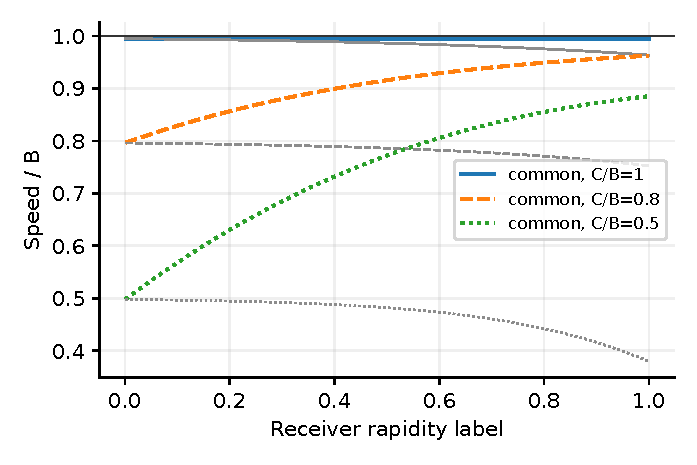
\includegraphics[width=0.96\textwidth,height=\textheight]{figures/review4_flow.pdf}
\caption{Bounded ballistic flow. Dark lines: common-reference arrival
velocities; gray lines: material-relative arrival velocities. The upper
bound is \(B=1\). Different receiver labels sample the same family of
radial rays.}
\end{figure}

\section{Astronomical distances, sizes and
brightness}\label{astronomical-distances-sizes-and-brightness}

\subsection{Distance definitions and a 1 Mpc
control}\label{distance-definitions-and-a-1-mpc-control}

An arcsecond measures angle; a parsec is a geometric parallax distance
convention (approximately 3.26 light-years). A light-year is a defined
length, not a statement that every photon travels that length each year.
Distinguish present physical separation, emission separation, path
length, a constant-speed travel-time estimate, angular diameter distance
\(D_A\), and luminosity distance \(D_L\). These are different
observables or inferences. If a stationary source and receiver are
actually 1 Mpc apart and the photon's \emph{independently measured}
average travel speed is \(\bar v\), then

\[D_{\rm inferred}=c_0\tau=D_{\rm actual}\frac{c_0}{\bar v}.\]

A photon that starts at \(c_0\) and slows exponentially in age,
\(v=c_0e^{-\gamma\tau}\), traverses
\(D=(c_0/\gamma)(1-e^{-\gamma\tau})\). If its arrival speed is half the
initial speed, \(D_{\rm inferred}/D=2\ln 2=1.38629\). Thus a true 1 Mpc
distance would be inferred as 1.386 Mpc from that measured travel time.
A globally changing characteristic speed which was faster in the past
than today instead gives the opposite sign in a direct time-of-flight
estimate. Real astronomical travel ages are usually unknown. An actual
redshift-distance prediction requires calculating observed frequency and
the chosen conventional inference procedure; a travel-time example is
not a distance measurement.

\subsection{Independent anchors and extreme-object
estimates}\label{independent-anchors-and-extreme-object-estimates}

The original distance audit (Z05) separates photometric
misclassifications from spectroscopically confirmed objects. The
reclassification of an apparent very distant source as a foreground
dwarf is evidence of the need for classification controls, not evidence
that all spectroscopically secure high-redshift objects are close. The
original audit tabulates the following ratios of alternative to
conventional angular-size distance. For unchanged measured angle, these
are also inferred physical-size ratios.

\begin{longtable}[]{@{}lrr@{}}
\toprule\noalign{}
Redshift & Static tired-light & Bounded propagation \\
\midrule\noalign{}
\endhead
\bottomrule\noalign{}
\endlastfoot
0.5 & 1.38 & 1.13 \\
1.0 & 1.80 & 1.30 \\
3.0 & 3.74 & 2.02 \\
10.603 & 12.74 & 4.75 \\
14.179 & 17.44 & 5.99 \\
\end{longtable}

The sign contradicts the proposed size reduction in these specific
models. It does not establish that every possible distance law has the
same sign. The original archive reports arithmetic comparisons, not fits
to individual galaxies.

The investigator's examples of WOH G64, HV 888, HV 11423, an Andromeda
red-supergiant candidate, Holmberg 15A, Phoenix A, and TON 618 motivate
an independent distance--size audit. For a star with unchanged measured
bolometric flux, temperature and extinction model, \(L=4\pi D_L^2 F\)
and \(R\propto D_L\) under the adopted stellar model. Halving an assumed
stellar distance halves the inferred radius and quarters the luminosity.
For an illustrative 1,540 solar-radius estimate, a factor of two
reduction would yield 770 solar radii. The Large Magellanic Cloud,
however, is anchored by late-type eclipsing binaries at \(49.59\pm0.09\)
(statistical) \(\pm0.54\) (systematic) kpc {[}4{]}. Such a major
distance change would need to account for the binary-based geometry as
well. Red-supergiant radii and dust environments remain model-dependent.

For a quasar broad-line virial estimator,
\(M_{\rm BH}\sim fR_{\rm BLR}v^2/G\) and a calibration
\(R_{\rm BLR}\propto L^{1/2}\) imply \(M_{\rm BH}\propto D_L\), holding
the measured velocity, geometry and calibration fixed. Thus an
illustrative 66-billion-solar-mass estimate for TON 618 would become 6.6
billion solar masses if the luminosity distance were ten times smaller.
This is a sensitivity example, not a revised measurement; reverberation
lags, redshift, flux and spectra need independent consistency checks.
Stellar-dynamical masses have different dependencies, and a quoted
horizon scale calculated from mass is not an independent image. The
extreme numerical mass estimates supplied in discussion are not adopted
here as verified contemporary catalog values. For geometric anchors, the
new theory must model propagation through parallax and binary-distance
experiments, not merely multiply distances by a universal correction.

\subsection{Estimator-specific inference and anchor-first
strategy}\label{estimator-specific-inference-and-anchor-first-strategy}

The proposed distance correction is not a single number. Report seven
quantities independently: emission separation \(D_e\), reception
separation \(D_a\), integrated physical path \(\ell\), constant-speed
travel-time proxy \(D_{\rm TOF}=c_0(T_a-T_e)\), angular distance
\(D_A\), reverse beam-area distance \(D_G\), and luminosity distance
\(D_L\). A redshift-based distance is an additional inference
\(D_{z,\mathcal M}\) conditional on a specified model \(\mathcal M\). In
a moving system none of these is guaranteed equal to the others. The
one-megaparsec control establishes a bias for \(D_{\rm TOF}\) only. Its
result cannot be used directly to rescale other distance indicators.

The six-report audit adds a useful nuisance-control relation:
uncorrected extinction \(A_\lambda\) changes the inferred inverse-square
distance by \(10^{A_\lambda/5}\). For instance 0.5 mag gives a factor
1.259. This is not evidence of C-01, and extinction must be separated
from physical aging. Calibrate nearby parallaxes, eclipsing binaries and
masers before modeling higher redshift. The independent report quotes an
NGC 4258 maser distance of 7.576 Mpc with statistical and systematic
uncertainties 0.082 and 0.076 Mpc; use the original publication and
covariance before incorporating the value into a likelihood. The Local
Group star cohort cannot be relocated independently of its host and
geometric anchors.

\begin{longtable}[]{@{}
  >{\raggedright\arraybackslash}p{(\columnwidth - 4\tabcolsep) * \real{0.3333}}
  >{\raggedright\arraybackslash}p{(\columnwidth - 4\tabcolsep) * \real{0.3333}}
  >{\raggedright\arraybackslash}p{(\columnwidth - 4\tabcolsep) * \real{0.3333}}@{}}
\toprule\noalign{}
\begin{minipage}[b]{\linewidth}\raggedright
Estimator or object cohort
\end{minipage} & \begin{minipage}[b]{\linewidth}\raggedright
Required model quantity
\end{minipage} & \begin{minipage}[b]{\linewidth}\raggedright
Conditional sensitivity
\end{minipage} \\
\midrule\noalign{}
\endhead
\bottomrule\noalign{}
\endlastfoot
WOH G64; HV 888; HV 11423 & \(D_L\), dust, temperature, atmosphere & At
fixed flux and temperature, \(R\propto D_L\) \\
LGGS J004520.67 + 414717.3 & Confirm identity, membership and spectrum &
No radius assigned without verified inputs \\
Holmberg 15A & \(D_A\), stellar velocities, orbit model &
\(M\propto D_A\) at fixed angular scale and velocities \\
Phoenix A & \(D_L\), accretion/feedback calibration & Fixed
Eddington-ratio luminosity proxy \(M\propto D_L^2\) \\
TON 618 & \(D_L\), broad-line luminosity and velocities & Single-epoch
virial \(M\propto D_L^{2a}\) for BLR slope \(a\) \\
\end{longtable}

The curated dossier reports alternative mass estimates for Holmberg 15A
(40 versus 21.6 billion solar masses) and model-dependent estimates for
Phoenix A and TON 618; these are source-reported sensitivity inputs, not
new measurements or a new distance determination. The fitted compression
slider in the independent distance explorer is not a derivation. Replace
it with actual 3D ray maps, a conserved transport model and joint
residuals. The target is simultaneous smaller physical distance and
smaller size without independently imposing the desired ratios.

\subsection{Two-direction optical geometry (Part
XXVI)}\label{two-direction-optical-geometry-part-xxvi}

Define \(D_A\) from source transverse area and observer solid angle and
\(D_G\) from receiver area and emitter solid angle. Let
\(A_T=dT_a/dT_e\), and let source and receiver calibrated clock readings
have local rates \(r_e=dt_e/dT\) and \(r_a=dt_a/dT\). The operational
stretch is \(A_c=(r_a/r_e)A_T\). Let \(Z_E=E_e/E_a\) be the physical
energy ratio of corresponding surviving packets and \(\mathcal T\) the
surviving fraction in the declared bundle. Use common physical energy
units for \(E_e,E_a\) and common calibrated area units, or report the
unit conversion explicitly. For isotropic emission with bolometric
luminosity per source-clock time,

\[F_a=\frac{L_e\mathcal T}{4\pi D_G^2 Z_E A_c},\qquad D_L=D_G\sqrt{Z_E A_c/\mathcal T}.\tag{O1}\]

If the numerical luminosity is quoted in source energy units \(e_e\) and
the numerical flux in receiver units \(e_a\) (each per calibrated clock
unit), multiply the right side for numerical flux by \(e_e/e_a\). A
luminosity distance inferred without making that conversion has an
additional factor \(\sqrt{e_a/e_e}\). Area-unit changes require their
own conversion. For broadband or multimode transport use the emitted
photon number distribution and integrate the actual detector response
times \(E_a\) and the corresponding ray-map and timing factors; one
scalar \(\mathcal T\) is valid only for the specified band or an
appropriately weighted bolometric model.

If \(\omega_e,\omega_a\) are physical local phase rates per \(T\)
sampled by the emitter and receiver, and \(\nu_e,\nu_a\) are their
respective reference clock frequencies per \(T\), a calibrated line
ratio for the same identified transition is
\(1+z_{\rm spec}=(\omega_e/\nu_e)/(\omega_a/\nu_a)\), with the emission
and detection conditions explicitly imposed. Motion requires phase
sampling along each material trajectory. Changes to the energy standard
or dressed-state absorption cannot be inferred from the frequency ratio
alone. In the following historical identical-clock control write
\(A=A_T=A_c\).

The energy, rate, and geometric factors must each follow from a physical
model. When identical endpoint standards give \(Z_E=A=1+z\), and the
chosen reciprocal static optical transport gives \(D_G=D_A\), the ratio
to the conventional distance-duality combination (in this paragraph
\(η=η_D\)) is

\[\eta=\frac{D_L}{(1+z)^2D_A}=\frac{1}{(1+z)\sqrt{\mathcal T}}.\]

The usual conventional reciprocity result in metric geometrical optics
has a different redshift relation between \(D_G\) and \(D_A\); we must
not silently import it into an alternative Euclidean ray model. In the
Part XXVI reciprocal test, a smooth refractive lens changes both
beam-area distances together. The example needs a refractive contrast of
about 28.7\% to reduce angular distance by 20\%. If \(D_A\) is 0.8 times
the reference angular distance at \(z=1\), matching the reference
\(D_L\) under the displayed assumptions requires
\(\mathcal T=(0.8/2)^2=0.16\) and gives \(\eta=1.25\). Loss alone cannot
match both independent distances and the same reference duality; it
would also require a physical account of deposited energy and any
radiation background. No such fitted attenuation law is derived here.

\emph{Historical figure (companion archive): Part XXVI optical
reciprocity test; both directional optical maps respond to lens
strength. Inherited figure.}

The exact three-dimensional spherical quadratic-screening example gives
central suppression of only 2.53 parts per million for the Part XI
galactic parameter \(q=0.00225\). Its positive angular-distance change
of approximately 7.89 parts per million over the illustrative ten-radius
path is \emph{defocusing}. This is the wrong sign for the hypothesized
large size reduction in this coupling. The reported reciprocal transfer
discrepancy is below \(1.1\times10^{-11}\); these are internal checks of
the selected optical geometry, not observational fit statistics.

\subsection{Directional three-dimensional optical
benchmark}\label{directional-three-dimensional-optical-benchmark}

The bounded flow above supplies a finite physical forward example with
no arbitrary distance-compression factor. In the isotropic rapidity
labels, transverse area at clock parameter \(\tau\) scales as
\((B\tau)^2\sinh^2\eta\) per unit solid angle about the center. For
infinitesimal beams with isotropic comoving directions, the transverse
separation per angular increment obeys the label-space Jacobi equation
\(J''=J\), \(J(0)=0\), \(J'(0)=1\), so \(J(\eta)=\sinh\eta\). This
equation describes the geometry of the \emph{material labels and ray
directions}, not a substance called spacetime. Reverse rays follow the
same label curves under the stated isotropy, no deflection, absence of
caustics and local angle assumptions. Consequently

\[D_A=B\tau_e\sinh\eta_s,\qquad D_G=B\tau_a\sinh\eta_s.\tag{O2}\]

For a central emitter, outward monotone radial path in common
coordinates and receiver ballistic trajectory, \(D_e=B T_e\tanh\eta_s\),
\(D_a=B T_a\tanh\eta_s\), \(\ell=D_a\), \(T_a=\tau_a\cosh\eta_s\); the
constant-speed travel-time proxy is \(B(T_a-T_e)\) in these normalized
units. Here \(T_e=\tau_e\). In the benchmark, \(B\) is the chosen
reference speed for the proxy, not necessarily the local emission
ceiling. For a curved or nonradial ray, the path is the integral of the
common-frame speed magnitude. More general optical maps require a 3D
transverse deviation solver with real matter gradients, lensing,
source/receiver area projections and extinction.

\begin{longtable}[]{@{}lr@{}}
\toprule\noalign{}
Quantity & Example (normalized) \\
\midrule\noalign{}
\endhead
\bottomrule\noalign{}
\endlastfoot
Emission separation \(D_e\) & 0.462117 \\
Reception separation \(D_a\) & 0.979680 \\
Path length \(\ell\) & 0.979680 \\
Constant-\(B\) travel proxy & 1.119981 \\
Angular distance \(D_A\) & 0.521095 \\
Reverse area distance \(D_G\) & 0.979680 \\
Luminosity distance \(D_L\) & 1.830347 \\
Energy ratio \(Z_E\) & 1.856658 \\
Calibrated arrival stretch \(A_c\) & 1.880039 \\
Common-coordinate stretch \(A_T\) & 2.119981 \\
Duality ratio \(D_L/(Z_E^2 D_A)\) & 1.018950 \\
\end{longtable}

The example uses unit photon survival, matching local energy and phase
standards, \(C/B=0.8\) and the finite gap stated above. The
\(Z_E\)-based duality ratio is a spectral duality ratio only when the
detector measures that same frequency ratio. Numerical integration of
the directional Jacobi equation in eight endpoint configurations agrees
with the analytic \(\sinh\eta\) factor to \(5.80\times10^{-13}\) in
normalized units. This is an optical geometry control, not a joint
likelihood or an independently measured distance correction. An active
Foundation 12 model must calibrate local geometric anchors, predict
independent flux/angle/timing/spectrum residuals for secure
high-redshift sources, and compare sizes or masses using the appropriate
estimator. The source classification of a foreground dwarf is a separate
observational test.

\section{Cosmic bubbles and the environmental
regulator}\label{cosmic-bubbles-and-the-environmental-regulator}

\subsection{Physical boundary versus geometric
convention}\label{physical-boundary-versus-geometric-convention}

The original cosmic-bubble investigations (Z01, Z11, Z12, Z22, Z23)
explore a physical domain, possible shell structures, exterior forces,
and birth/death of domains in a larger cosmos. A boundary in a density
or field distribution is different from a survey horizon or a
mathematical surface. The archive reports no statistically validated
detection of a neighboring bubble. The following geometries are
hypothetical alternatives: distributed matter within a domain,
low-density cavity enclosed by a shell, nonuniform exterior mass, or no
material boundary at all. The total age and size of a larger physical
cosmos are not inferred from the radius or history of an observable
region. Stellar ages and chronometer data still impose constraints on
local physical history. Formation, stability and evolution of any wall
require a matter dynamics model and energy budget; a static shell alone
proves none of these.

\subsection{Finite-range collective response (Part
XXVII)}\label{finite-range-collective-response-part-xxvii}

Use a scalar environmental variable \(I\) with a positive kinetic term
and finite range \(\lambda\). In a static limit,

\[(-\nabla^2+\lambda^{-2})I=g\rho,\]

\[I(\mathbf{x})=\frac{g}{4\pi}\int \rho(\mathbf{x}')\frac{e^{-|\mathbf{x}-\mathbf{x}'|/\lambda}}{|\mathbf{x}-\mathbf{x}'|}\,d^3x'.\]

The second expression is a static equilibrium Green function, not
instantaneous signaling. A dynamical completion may use
\(C_I^{-2}\partial_T^2 I-\nabla^2 I+\lambda^{-2}I=g\rho\) with retarded
conditions. A reduced positive electromagnetic mode Lagrangian with a
kinetic coefficient proportional to \(1+\alpha I^2\) gives a
characteristic speed of the form

\[C(I)=\frac{C_*}{\sqrt{1+\alpha I^2}},\qquad \alpha\geq0.\]

The mass-gap coefficient must be chosen consistently with the kinetic
normalization. For example, for a real reduced mode \(a\),
\(\mathcal L_a=\tfrac12(1+\alpha I^2)[(\partial_T a)^2-\Omega^2a^2]-\tfrac12 C_*^2|\nabla a|^2\)
gives the stated fixed-gap dispersion in a constant background. This
demonstrates a hyperbolic mode with positive quadratic energy in that
background; it is not a proof of stability of a complete coupled vector,
matter and gravitational theory. In particular, the regulator field has
its own characteristic \(C_I\). If it is faster, \(C(I)\) is not the
all-sector causal ceiling. The constitutive form and reference \(C_*\)
are assumptions; normalizing the model to \(c_0\) does not derive the
observed numerical value from cosmic mass. A mechanical inertia law must
also be independently specified and tested.

For an infinitesimally thin shell of mass \(M\) and radius \(R\), let
\(q=R/\lambda\) and \(x=r/R\). Direct angular integration gives

\[I(0)=\frac{gM}{4\pi R}e^{-q},\]

\[\frac{I(r)}{I(0)}=\begin{cases}\dfrac{\sinh(qx)}{qx},&x\leq1,\\[4pt]\dfrac{\sinh(q)}{q}\dfrac{e^{-q(x-1)}}{x},&x\geq1.\end{cases}\]

The interior response is nonzero even where the Newtonian shell force
vanishes. The finite-range scalar gradient need not vanish except at the
center or in the long-range symmetric limit; ordinary shell theorem does
not apply to every modified force. For the illustrative normalization
\(\alpha I(0)^2=1\) and \(C(0)=c_0\), \(C_*=\sqrt2 c_0\). Six range
values were checked numerically in Part XXVII.

\begin{longtable}[]{@{}rrrr@{}}
\toprule\noalign{}
\(R/\lambda\) & \(I(R)/I(0)\) & \(C(R)/c_0\) & \(C(2R)/c_0\) \\
\midrule\noalign{}
\endhead
\bottomrule\noalign{}
\endlastfoot
0.01 & 1.000017 & 0.999992 & 1.267419 \\
0.1 & 1.001668 & 0.999167 & 1.288118 \\
0.5 & 1.042191 & 0.979132 & 1.348465 \\
1 & 1.175201 & 0.916487 & 1.382287 \\
2 & 1.813430 & 0.682906 & 1.403685 \\
5 & 14.840642 & 0.095078 & 1.412449 \\
\end{longtable}

\emph{Historical figure (companion archive): Part XXVII shell-regulator
example. Curves are normalized model predictions, not measurements of
the universe or its exterior.}

The outside asymptote is \(\sqrt2 c_0\) under this chosen normalization.
It is not evidence of a faster exterior universe. Part XXVII reports
independent angular quadratures consistent with the analytic kernel to
relative discrepancy \(1.223\times10^{-12}\). A ray of fixed positive
frequency in the static profile slows toward the wall and speeds up on
leaving it. Thus the candidate succeeds in producing a field-dependent
characteristic but \textbf{fails the strict global no-reacceleration
requirement} and cannot by itself generate redshift. It also does not
yet derive the mechanical acceleration resistance envisaged in C-01.
These are constraints on the model, not reasons to erase the motivating
hypothesis.

\subsection{Void benchmark and experimental
interpretation}\label{void-benchmark-and-experimental-interpretation}

For an infinite spatial domain containing uniform finite density with
the finite-range static kernel, \(I_{\rm ref}=g\rho_0\lambda^2\).
Removing matter in a sphere of radius \(b\) removes a fraction of the
center response

\[f(s)=1-(1+s)e^{-s},\qquad s=b/\lambda.\]

At \(\alpha I_{\rm ref}^2=1\), the center speed changes by
\(\sqrt{2/[1+(1-f)^2]}-1\). For \(s=0.01,0.1,1\), this is approximately
\(2.4834\times10^{-5}\), \(0.00234215\) and \(0.13910987\). The infinite
uniform distribution is a mathematical benchmark with a convergent
kernel, not a statement about finite total cosmic mass. Real voids
contain matter, move and have structure; no observed speed variation is
claimed. A comparison must predict changes in clock ratios, signal
travel times, phase, and gravity versus electromagnetic propagation. If
every sector and standard changes together, the coordinate-speed change
may not be independently observable.

\section{Photon aging: Part XXVIII bounded
control}\label{photon-aging-part-xxviii-bounded-control}

\subsection{Motivation and model}\label{motivation-and-model}

The previous shell result separates the local emission ceiling from the
post-emission slowing mechanism. Can the simplest passive momentum-loss
mechanism yield the desired aging, redshift and arrival behavior?
Consider a homogeneous stationary environment with fixed \(C\), positive
rest energy \(E_m=\hbar\Omega=m_\gamma C^2\) and a single forward packet
with momentum \(p>0\). Adopt an explicit effective drag law, not a
microscopic interaction derivation:

\[\begin{aligned}E(p)&=\sqrt{C^2p^2+E_m^2},\\v&=\frac{\partial E}{\partial p}=\frac{C^2p}{E},\\\dot p&=-\gamma p,\quad \gamma>0.\end{aligned}\]

This is an open packet description in a selected environmental rest
frame; it is not Lorentz invariant as written. Define the dimensionless
momentum \(u=Cp/E_m\), initial \(u_e>0\), and age \(\tau=T-T_e\). Then
\(u=u_e e^{-\gamma\tau}\) and

\[\frac{v}{C}=\frac{u}{\sqrt{1+u^2}},\qquad \frac{d v}{dT}=-\frac{\gamma v}{1+u^2}<0.\]

The derivative demonstrates strict monotonicity in the stationary
medium. The energy and momentum lost by the packet are

\[\begin{aligned}\dot E&=-\gamma pv=-\gamma E\left(1-\frac{E_m^2}{E^2}\right),\\\dot E_{\rm bath}&=+\gamma pv,\quad \dot p_{\rm bath}=+\gamma p.\end{aligned}\]

The bath ledger balances energy and momentum formally but does not
supply physical bath degrees of freedom, their recoil, entropy
production, noise or stress. A full conservative completion must derive
\(\gamma\), implement local exchange, and test whether this collinear
continuous-loss approximation can avoid scattering, line broadening and
excess heat. A passive bath at nonzero temperature may return energy to
packets; deterministic irreversible loss is a macroscopic effective
assumption. The calculated wave retains a positive rest energy at late
time, not a demonstrated dark-matter population.

\subsection{Exact distance and redshift
relations}\label{exact-distance-and-redshift-relations}

Integrating the speed yields

\[D(\tau)=\frac{C}{\gamma}\left[\operatorname{arsinh}u_e-\operatorname{arsinh}(u_e e^{-\gamma\tau})\right].\]

The packet approaches the finite travel distance
\(D_{\max}=(C/\gamma)\operatorname{arsinh}u_e\) as its momentum tends to
zero. This is a packet-range result under eternal drag, not an
all-sector causal horizon. For stable identical atomic references and no
endpoint motion, \(1+z=E_e/E_a\). Set \(\epsilon=E_m/E_e\), with
\(0<\epsilon<1\). Then

\[\boxed{\frac{v_a}{C}=\sqrt{1-\epsilon^2(1+z)^2}}\]

for \(\epsilon(1+z)<1\). The allowed redshift has upper limiting value
\(1/\epsilon-1\). The fractional speed deficit can be evaluated
accurately without subtractive cancellation as

\[1-\frac{v_a}{C}=\frac{\epsilon^2(1+z)^2}{1+\sqrt{1-\epsilon^2(1+z)^2}}.\]

For small \(\epsilon\), its leading value is \(\epsilon^2(1+z)^2/2\).
This is a new conditional obstruction: a tiny fixed gap plus modest
energy loss does not yield substantial speed loss. Large speed reduction
requires the packet energy to approach the rest-energy gap. At
\(v_a=C/2\), \(E_a=2E_m/\sqrt3\) and \(1+z=\sqrt3/(2\epsilon)\). For
\(\epsilon=10^{-8}\) this would require a frequency ratio of about
\(8.66\times10^7\), not an ordinary optical redshift of order unity.
Positive mass alone is therefore not sufficient to derive substantial
tired-light deceleration. Conversely, a large photon gap would create
strong chromatic effects and conflict with existing mass tests in the
corresponding dispersion model.

\begin{longtable}[]{@{}
  >{\raggedleft\arraybackslash}p{(\columnwidth - 6\tabcolsep) * \real{0.2500}}
  >{\raggedleft\arraybackslash}p{(\columnwidth - 6\tabcolsep) * \real{0.2500}}
  >{\raggedleft\arraybackslash}p{(\columnwidth - 6\tabcolsep) * \real{0.2500}}
  >{\raggedleft\arraybackslash}p{(\columnwidth - 6\tabcolsep) * \real{0.2500}}@{}}
\toprule\noalign{}
\begin{minipage}[b]{\linewidth}\raggedleft
Initial gap fraction \(\epsilon\)
\end{minipage} & \begin{minipage}[b]{\linewidth}\raggedleft
Redshift \(z\)
\end{minipage} & \begin{minipage}[b]{\linewidth}\raggedleft
Arrival speed deficit \(1-v_a/C\)
\end{minipage} & \begin{minipage}[b]{\linewidth}\raggedleft
Energy transferred
\end{minipage} \\
\midrule\noalign{}
\endhead
\bottomrule\noalign{}
\endlastfoot
\(10^{-2}\) & 1 & \(2.0002\times10^{-4}\) & 50\% \\
\(10^{-4}\) & 1 & \(2.0000\times10^{-8}\) & 50\% \\
\(10^{-8}\) & 1 & \(2.0000\times10^{-16}\) & 50\% \\
\(10^{-16}\) & 1 & \(2.0000\times10^{-32}\) & 50\% \\
\end{longtable}

These gap fractions are illustrative, not measured photon masses. The
comparison changes the gap-to-emission-energy ratio while holding
observed redshift fixed.

\emph{Historical figure (companion archive): Part XXVIII benchmark.
Fractional speed deficit versus energy redshift for four positive gap
fractions. Large redshift need not entail large speed loss.}

\subsection{A stationary aging law does not reproduce supernova time
dilation}\label{a-stationary-aging-law-does-not-reproduce-supernova-time-dilation}

For fixed stationary endpoints separated by \(D<D_{\max}\), equal
emission energies and identical environmental conditions, the travel age
\(\tau_D\) follows from the distance equation. It has no dependence on
the absolute emission time. Therefore \(T_a=T_e+\tau_D\), and

\[\frac{dT_a}{dT_e}=1.\]

Even when each packet loses half its energy (\(z=1\)), successive
identical packet intervals are not stretched. A light curve may broaden
through frequency-dependent dispersion, but this is not a general
achromatic factor \(1+z\) multiplying its intrinsic time axis. A moving
source or a medium that evolves in absolute time can change this
conclusion; so can a physical source clock response, if independently
justified. The Dark Energy Survey measured a stretching exponent
\(b=1.003\pm0.005\) (statistical) \(\pm0.010\) (systematic), using a
model proportional to \((1+z)^b\) for 1,504 Type Ia supernovae {[}5{]}.
This places a strong observational burden on the stationary loss-only
subclass, not on every model including recession and time evolution.

\subsection{Can drag prevent exterior
reacceleration?}\label{can-drag-prevent-exterior-reacceleration}

In a slowly varying medium with dispersion \(\omega^2=C^2k^2+\Omega^2\),
set \(u=Ck/\Omega\). Along the ray the algebraic group velocity
satisfies

\[\frac{d\ln v_g}{dT}=\frac{d\ln C}{dT}+\frac{1}{1+u^2}\frac{d\ln u}{dT}.\]

Here the total derivatives include environmental change and the
Hamiltonian momentum equation plus any drag; they cannot be chosen
independently. To enforce monotonic slowing during a rise of \(C\), the
second term must be sufficiently negative. In the high-frequency regime
\(u\gg1\), the factor \(1/(1+u^2)\) strongly suppresses momentum-loss
effects on speed. Moderate drag cannot generally compensate a
substantial rise in the local characteristic while leaving the spectrum
in the same band. An additional history-dependent constitutive
mechanism, or a dynamic common field is needed; changing the charter
would require an explicit investigator decision. No such mechanism has
been independently derived by imposing a minimum of previous and current
speeds. The C-01 result and the new drag benchmark jointly constrain a
viable theory.

\subsection{New calculation
verification}\label{new-calculation-verification}

The included Python program compares the closed distance equation with
adaptive numerical integration at 19 combinations of positive gap
fraction and redshift. Maximum absolute discrepancy in units
\(C/\gamma\) is \(5.32907\times10^{-15}\). It checks monotone packet
energy, the arithmetic energy ledger and equal stationary pulse
intervals. The CSV reports the stable speed-deficit formula. The bath is
not simulated, so the bookkeeping test is not proof of a microscopic
conservation law. This benchmark is an analytical and numerical test of
a deliberately restricted ansatz, not a claim of a derived universal
photon-aging interaction.

\section{Part XXX --- exact monotonicity and energy requirements at a
domain
wall}\label{part-xxx-exact-monotonicity-and-energy-requirements-at-a-domain-wall}

\subsection{Motivation and scope}\label{motivation-and-scope}

The C-01 shell calculation allows a higher local characteristic speed
outside a restrictive wall. The research charter requires a photon to
slow after emission, so we need a mechanism that carries its propagation
history through a changing environment. This section derives a necessary
energy bound and an exact controlled crossing test. It does not propose
that the actual universe has the illustrative wall or that fixed-gap
drag is the final aging mechanism. The result is a diagnostic for future
candidates.

\subsection{Static wall with a fixed positive
gap}\label{static-wall-with-a-fixed-positive-gap}

Write the packet Hamiltonian and signed momentum equation in one
dimension as

\[\begin{aligned}E(x,p)&=\sqrt{C^2(x)p^2+\Delta^2},\\\dot x&=v=\partial_pE,\quad \dot p=-\partial_x E-\gamma p.\end{aligned}\]

where \(p>0\), \(\Delta>0\) is a constant rest-energy gap, and
\(\gamma\geq0\) is a momentum relaxation rate. This is a fixed-gap
control, not fixed invariant rest mass if \(C\) varies. The static field
performs no net Hamiltonian work on \(E\): the Hamiltonian terms cancel
in the total derivative. Define \(q=\Delta^2/E^2\). Then

\[\dot E=-\gamma pv=-\gamma E(1-q),\quad v=C\sqrt{1-q},\]

\[\frac{d\ln v}{dT}=\frac{d\ln C}{dT}-\gamma q.\]

In a region where \(C\) increases along the path, monotone slowing
requires \(\gamma q\geq d\ln C/dT\). Small \(q\) makes the slowing
efficiency very weak. This is independent of any prescribed
maximum-speed clamp. The energy extracted is recorded as a reservoir
intake \(\dot B=\gamma E(1-q)\); \(E+B\) is constant in this reduced
model. The static wall is external and the momentum receiver is not
simulated, so this is not a closed matter-field action.

\subsection{Endpoint energy bound}\label{endpoint-energy-bound}

Let \(s=C_1/C_e>1\), \(\varepsilon=\Delta/E_e\in(0,1)\) and
\(r=E_1/E_e\). Nonincreasing speed necessarily gives

\[C_1\sqrt{1-\varepsilon^2/r^2}\leq C_e\sqrt{1-\varepsilon^2}.\]

Solving for the largest possible retained energy yields

\[\boxed{r\leq \frac{\varepsilon s}{\sqrt{s^2-1+\varepsilon^2}}.}\]

Equality gives the same final and initial speed, not proof of
monotonicity throughout the journey. In a fixed-gap packet the energy
cannot fall below \(\Delta\). The bound shows that even a modest
increase in \(C\) can force the arrival energy close to the gap. For
\(s=1.1\) and \(\varepsilon=10^{-16}\), the retained fraction can be at
most \(2.4004\times10^{-16}\). The required loss is nearly all the
emitted energy. If a photon remains in the original observational band,
passive momentum drag in this fixed-gap model cannot provide such a
crossing.

\begin{longtable}[]{@{}
  >{\raggedright\arraybackslash}p{(\columnwidth - 4\tabcolsep) * \real{0.3333}}
  >{\raggedleft\arraybackslash}p{(\columnwidth - 4\tabcolsep) * \real{0.3333}}
  >{\raggedleft\arraybackslash}p{(\columnwidth - 4\tabcolsep) * \real{0.3333}}@{}}
\toprule\noalign{}
\begin{minipage}[b]{\linewidth}\raggedright
Local ceiling ratio \(s\)
\end{minipage} & \begin{minipage}[b]{\linewidth}\raggedleft
Max. retained fraction, gap fraction \(10^{-6}\)
\end{minipage} & \begin{minipage}[b]{\linewidth}\raggedleft
Max. retained fraction, gap fraction \(10^{-16}\)
\end{minipage} \\
\midrule\noalign{}
\endhead
\bottomrule\noalign{}
\endlastfoot
1.001 & \(2.238\times10^{-5}\) & \(2.238\times10^{-15}\) \\
1.01 & \(7.124\times10^{-6}\) & \(7.124\times10^{-16}\) \\
1.10 & \(2.400\times10^{-6}\) & \(2.400\times10^{-16}\) \\
\(\sqrt{2}\) & \(1.414\times10^{-6}\) & \(1.414\times10^{-16}\) \\
\end{longtable}

\emph{Historical figure (companion archive): Calculated endpoint upper
bounds. A greater rise in the local characteristic, or a smaller initial
gap fraction, demands a smaller retained energy fraction. This is a
restricted theoretical control.}

\subsection{Linear-wall crossing: exact solution and
feasibility}\label{linear-wall-crossing-exact-solution-and-feasibility}

Normalize \(C_e=E_e=1\) and wall thickness to one; dimensionless time is
wall thickness divided by \(C_e\). Let \(C(x)=1+\kappa x\) for
\(0\leq x\leq1\), with \(\kappa=s-1>0\). Put
\(y=\operatorname{arcosh}(E/\Delta)\), so \(v=C\tanh y\). Dividing the
energy equation by \(\dot x>0\) gives \(dy/dx=-\gamma/C(x)\). At
constant drag the solution is

\[y(x)=y_e-\frac{\gamma}{\kappa}\ln(1+\kappa x),\qquad y_e=\operatorname{arcosh}(1/\varepsilon).\]

It is valid until the momentum vanishes. To arrive at the far wall with
positive speed requires \(\gamma<\kappa y_e/\ln s\). From the speed
derivative, monotone slowing already at entry requires
\(\gamma\geq\kappa\sinh y_e\cosh y_e\). Since \(y(x)\) decreases, that
lower bound suffices for monotonicity while the photon continues moving.
Both conditions can hold only if

\[\boxed{\ln s<\frac{y_e}{\sinh y_e\cosh y_e}=\frac{\varepsilon^2\operatorname{arcosh}(1/\varepsilon)}{\sqrt{1-\varepsilon^2}}.}\]

As the positive gap fraction becomes very small, the allowed ceiling
increase scales as \(\varepsilon^2\ln(2/\varepsilon)\). For
\(\varepsilon=0.1\) and \(s=1.2\), monotonic entry requires
\(\gamma\geq19.89975\), but a crossing requires \(\gamma<3.28345\). No
constant drag satisfies both. Even a drag that delivers a slower photon
at the far wall may violate the required trajectory history by allowing
initial acceleration.

\begin{longtable}[]{@{}
  >{\raggedleft\arraybackslash}p{(\columnwidth - 8\tabcolsep) * \real{0.2000}}
  >{\raggedright\arraybackslash}p{(\columnwidth - 8\tabcolsep) * \real{0.2000}}
  >{\raggedleft\arraybackslash}p{(\columnwidth - 8\tabcolsep) * \real{0.2000}}
  >{\raggedleft\arraybackslash}p{(\columnwidth - 8\tabcolsep) * \real{0.2000}}
  >{\raggedleft\arraybackslash}p{(\columnwidth - 8\tabcolsep) * \real{0.2000}}@{}}
\toprule\noalign{}
\begin{minipage}[b]{\linewidth}\raggedleft
Constant drag
\end{minipage} & \begin{minipage}[b]{\linewidth}\raggedright
Traverses wall?
\end{minipage} & \begin{minipage}[b]{\linewidth}\raggedleft
Final position
\end{minipage} & \begin{minipage}[b]{\linewidth}\raggedleft
Final speed
\end{minipage} & \begin{minipage}[b]{\linewidth}\raggedleft
Final energy
\end{minipage} \\
\midrule\noalign{}
\endhead
\bottomrule\noalign{}
\endlastfoot
0 & Yes & 1 & 1.193985 & 1.000000 \\
0.2 & Yes & 1 & 1.191348 & 0.834252 \\
2 & Yes & 1 & 0.989129 & 0.176619 \\
19.89975 & No & 0.152700 & \(\simeq0\) & 0.100000 \\
\end{longtable}

The last solution asymptotically stops within the wall. The \(\gamma=2\)
case ends below its initial speed but initially accelerates. The four
independently integrated trajectories agree with the analytic rapidity
expression to \(4.19\times10^{-12}\) maximum absolute error, and the
integrated energy ledger closes to \(8.72\times10^{-12}\). Sixteen
endpoint identities and all reachability checks pass. No real-wall
normalization, microscopic bath or observational inference is claimed.

\emph{Historical figure (companion archive): Independent numerical
integrations of the linear wall. The strong drag required for
monotonicity stops the photon inside the wall.}

\subsection{Variable gap: constructive design
target}\label{variable-gap-constructive-design-target}

If \(\Delta\) varies along a path, then the exact algebraic identity is

\[\frac{d\ln v}{dT}=\frac{d\ln C}{dT}+\frac{q}{1-q}\left(\frac{d\ln E}{dT}-\frac{d\ln\Delta}{dT}\right).\]

A possible candidate could increase a positive effective gap while
accounting for the energy required to dress the radiation. Endpoint
monotonicity requires

\[\frac{\Delta_1}{E_e}\geq r\sqrt{1-\frac{1-\varepsilon^2}{s^2}}.\]

For \(s=1.1\), initial gap fraction \(10^{-16}\), and \(r=1/2\), the
final gap must be at least 0.2083 of the original energy. For optical or
radio radiation that is a significant constitutive change, with
associated dispersion and atomic/detector constraints. This is an
explicit target for a dynamic gap or alternative history-state theory,
not a measured gap or a permission to change fundamental invariant
photon mass. A microscopic theory must distinguish invariant mass from
environmental dressing, derive emission and detection, and account for
work from the regulator and reservoir. A reversible wall effect cannot
substitute for irreversible aging.

\textbf{Part XXX decision.} Retain C-01's physical ceiling and the
research requirement of monotone post-emission slowing. Use the
fixed-gap wall as a quantitative exclusion control for candidate
mechanisms; do not promote constant drag as the physical solution. Next
derive a causal, energy-and-momentum-accounted history field with a
positive photon mass and independent emission and wall boundary
conditions.

\section{Part XXXI --- irreversible momentum-to-gap conversion with
finite capacity and
recoil}\label{part-xxxi-irreversible-momentum-to-gap-conversion-with-finite-capacity-and-recoil}

\textbf{Status:} retained Part XXXI analytical and executed reduced
packet model, not a microscopic photon theory or an observational fit.
The twelve foundations and the investigator's C-01 clarification are
unchanged. This follows the exact fixed-gap restriction in Part XXX. The
central question remains what establishes the initial local emission
ceiling, and why a packet subsequently slows rather than acquiring a
higher speed when its environment changes.

\subsection{Candidate physical mechanism and declared
assumptions}\label{candidate-physical-mechanism-and-declared-assumptions}

Retain a positive reference gap \(\Delta_0=m_0 C_e^2\) with \(m_0>0\)
and \(C_e\) the reference characteristic speed. Introduce a physical
dressing/conversion coordinate \(a\geq0\) (momentum units) and
\(\Delta(a)=\Delta_0+\beta a\), with \(\beta>0\) in speed units. The
effective gap is \textbf{not} identified with a changing fundamental
invariant photon mass. The conversion law is a phenomenological
irreversible constitutive law; a local field theory generating it
remains open. A small bare gap can make the initial group speed
arbitrarily close to the characteristic, but an exact finite-energy
equality remains unresolved. Adopt one spatial coordinate and constant
ordering time \(T\). The illustrative wall is a prescribed static
regulator, not a self-consistent bubble; its material support receives
the wall reaction momentum. The local characteristic is \(C(x)>0\).
Assume positive forward momentum throughout the benchmark.

The reduced packet Hamiltonian is

\[\begin{aligned}E&=\sqrt{C(x)^2p^2+\Delta(a)^2},\\v&=\partial_p E=\frac{C^2p}{E},\\E_a&=\frac{\beta\Delta}{E},\quad E_x=\frac{CC'p^2}{E}.\end{aligned}\]

An effective finite receiver has momentum \(P=a\) (zero initially),
inertial coefficient \(M>0\), recoil energy \(P^2/(2M)\) and velocity
\(U=P/M\). This nonrelativistic receiver is appropriate only for small
\(U\) in the selected normalization. \(Q\) is irreversible internal
energy deposited into that receiver. This is a lumped receiver
approximation along the trajectory, not a solved spatial bath, nor a
claim of instantaneous transport across the universe. It deliberately
separates the internal dressing coordinate (whose energy is already
included in \(E\)) from the deposited heat. Let \(A\) be the energy
release per transferred momentum:

\[A=v-E_a-U.\]

For mobility \(K>0\) and capacity \(a_{\max}>0\), choose the one-way
conversion law

\[\dot a=K\max(A,0)\max(1-a/a_{\max},0).\]

This supplies a dissipative branch with nonnegative heat production. It
is not a speed clamp: it depends on the energetic driving force and
capacity, not on the sign of the desired speed derivative. Its absence
of reverse conversion requires an underlying physical rectification
process, not yet derived; detailed balance, noise and finite-temperature
emission remain tasks. The evolution equations are

\[\dot x=v,\qquad \dot p=-E_x-\dot a,\qquad \dot P=\dot a,\qquad \dot Q=A\dot a,\qquad \dot W=E_x,\]

where \(W\) is reaction momentum received by the externally held wall.
\(P=a\) and \(W(0)=Q(0)=0\). A finite wall recoil model would require
its own dynamics and energy; \(W\) is a ledger for the fixed-wall
approximation, not a claim that a finite freely moving wall accepts
momentum at zero energy cost.

\subsection{Conservation, passivity and
monotonicity}\label{conservation-passivity-and-monotonicity}

The Hamiltonian work terms cancel for a static wall, leaving

\[\begin{aligned}\dot E&=-(v-E_a)\dot a,\\\frac{d}{dT}\left(E+\frac{P^2}{2M}+Q\right)&=0,\\\frac{d}{dT}(p+P+W)&=0.\end{aligned}\]

Whenever conversion occurs, \(A>0\), so \(\dot Q\geq0\) and
\(\dot E\leq0\). At zero affinity or capacity exhaustion the exchange
stops. The model does not require an unbounded heat sink in a
single-packet calculation. It does not establish a steady cosmological
bath. At fixed \(a\) the positive gap gives \(v<C\) for every finite
positive \(p\); the fastest causal characteristic of a full coupled
field theory has not yet been established.

Differentiating the velocity along the evolution gives the exact
trajectory identity

\[\boxed{\dot v=\frac{v^2C'}{C}-\frac{C^2\Delta(\Delta+\beta p)}{E^3}\dot a.}\]

The first term is the conservative wall response; the second is recoil
plus internal dressing. In a uniform environment the second term is
nonpositive. For a rising wall, nonincreasing speed requires

\[\dot a\geq\frac{v^2 C'E^3}{C^3\Delta(\Delta+\beta p)}\qquad(C'>0).\]

This is a necessary and sufficient \emph{instantaneous} condition under
this reduced model. It is evaluated after solving the dynamics, not used
to force the velocity. When the initial gap is very small, an abrupt
positive gradient can overwhelm the conversion response; the rate also
falls toward zero when capacity or affinity is exhausted. Unlike
fixed-gap drag, \(\beta p\) can substantially increase the slowing term
after conversion grows. The model does not establish monotonicity across
arbitrary environments.

At arrival, for \(s=C_1/C_e>1\), the Part XXX endpoint condition
generalizes to

\[\Delta_1\geq E_1\sqrt{1-(v_e/C_1)^2}.\]

This is a useful gap budget, not sufficient to guarantee monotonic
history. Since \(a\leq a_{\max}\),
\(\Delta_1\leq\Delta_0+\beta a_{\max}\). For a monotone-in-position wall
with \(C\leq C_1\) and forward motion, the integrated energy equation
implies \(E_1\geq E_e-C_1 a_{\max}\), since \(v-E_a\leq C_1\) during
conversion. Combining the two yields the necessary finite-capacity
condition

\[\boxed{E_e\leq C_1 a_{\max}+\frac{\Delta_0+\beta a_{\max}}{\sqrt{1-(v_e/C_1)^2}}.}\]

The bound is implicit because \(v_e\) depends on \(E_e\). At fixed
\(s>1\), as \(E_e\) becomes large the denominator tends to
\(\sqrt{1-s^{-2}}>0\). Hence any fixed finite capacity excludes
monotonic crossing for sufficiently large emission energy, no matter how
large the mobility. This is an analytical design constraint: a universal
model needs an independently justified energy-dependent capacity,
multiple local exchange degrees of freedom, or another mechanism. It is
not a license to tune a separate parameter per observed frequency.

\subsection{Executed smooth-wall
benchmark}\label{executed-smooth-wall-benchmark}

Use units \(C_e=1\), reference packet energy \(E_e=1\) and wall
thickness \(L_w=1\); time unit \(L_w/C_e\), momentum unit \(E_e/C_e\).
At \(x=-0.3\), set \(a=P=Q=W=0\) and \(p=\sqrt{1-\Delta_0^2}\) with
\(\Delta_0=10^{-6}\). For \(0\leq x\leq1\) set \(C=1+0.2(3x^2-2x^3)\),
extended constantly on each side. Choose \(\beta=1\), \(K=1\),
\(M=100\), \(a_{\max}=2\). These are dimensionless example parameters,
not cosmological calibrations. The lead region permits the same physical
conversion before the wall, without a special change of law at the
boundary. Integrate the autonomous reduced ODEs until \(x=1\) or
stopping, with adaptive tolerances, dense samples and a refined repeat.

\begin{longtable}[]{@{}lr@{}}
\toprule\noalign{}
Quantity & Baseline result \\
\midrule\noalign{}
\endhead
\bottomrule\noalign{}
\endlastfoot
Arrival time & 1.445830 \\
Initial group speed / \(C_e\) & 0.9999999999995 \\
Final group speed / \(C_e\) & 0.822104 \\
Final characteristic / \(C_e\) & 1.2 \\
Final packet energy / \(E_e\) & 0.695303 \\
Final effective gap / \(E_e\) & 0.506501 \\
Required minimum final gap / \(E_e\) & 0.384343 \\
Deposited heat / \(E_e\) & 0.303415 \\
Receiver recoil energy / \(E_e\) & 0.001283 \\
Wall reaction momentum / \((E_e/C_e)\) & 0.096548 \\
Maximum sampled \(\dot v\) & \(-1.0\times10^{-6}\) \\
\end{longtable}

The packet crosses with positive momentum, retains 69.53\% of its
original energy, and has no sampled positive speed derivative in the
baseline and refined trajectories. This is materially different from the
fixed-gap restriction, but does not certify the continuous trajectory by
interval arithmetic or show a physically realizable microscopic
coupling. It also requires a large dressed gap: about 72.85\% of arrival
energy. It is not automatically an observable ordinary photon of the
same spectral band. The energy sum includes the gap only once. The
receiver reaches a speed about 0.0051 in reference units, consistent
with the selected nonrelativistic recoil approximation.

\emph{Historical figure (companion archive): Group velocity across the
wall in the reduced model. The no-exchange, low-capacity and fixed-gap
controls reaccelerate in parts of the path.}

\emph{Historical figure (companion archive): Packet and receiver energy
ledger. The gap is part of packet energy, not an additional contribution
to the conserved total.}

\subsection{Controls, sensitivity and
limitations}\label{controls-sensitivity-and-limitations}

Every named case below used the same constitutive equations, varying
only indicated inputs. Energy columns are fractions of that run's own
emission energy; group velocities are relative to the same initial
characteristic. Monotonicity is diagnosed by maximum sampled analytical
derivative, not just endpoint speed. A case with a smaller final speed
can still reaccelerate during flight.

\begin{longtable}[]{@{}
  >{\raggedright\arraybackslash}p{(\columnwidth - 6\tabcolsep) * \real{0.2500}}
  >{\raggedleft\arraybackslash}p{(\columnwidth - 6\tabcolsep) * \real{0.2500}}
  >{\raggedleft\arraybackslash}p{(\columnwidth - 6\tabcolsep) * \real{0.2500}}
  >{\raggedleft\arraybackslash}p{(\columnwidth - 6\tabcolsep) * \real{0.2500}}@{}}
\toprule\noalign{}
\begin{minipage}[b]{\linewidth}\raggedright
Test
\end{minipage} & \begin{minipage}[b]{\linewidth}\raggedleft
Retained energy
\end{minipage} & \begin{minipage}[b]{\linewidth}\raggedleft
Final speed
\end{minipage} & \begin{minipage}[b]{\linewidth}\raggedleft
Maximum sampled \(\dot v\)
\end{minipage} \\
\midrule\noalign{}
\endhead
\bottomrule\noalign{}
\endlastfoot
Baseline & 0.695303 & 0.822104 & \(-1.0\times10^{-6}\) \\
Bare gap \(10^{-16}\) & 0.695302 & 0.822104 & \(-1.0\times10^{-16}\) \\
No exchange & 1.000000 & 1.200000 & 0.331516 \\
Fixed gap (\(\beta=0\)) & \(\simeq10^{-6}\) & 0.009415 & 0.331516 \\
No lead region & 0.685254 & 0.862014 & 0.005392 \\
Capacity 0.1 & 0.905467 & 1.192659 & 0.327398 \\
Capacity 0.3 & 0.762609 & 1.111477 & 0.240912 \\
Capacity 0.5 & 0.709826 & 0.991140 & 0.102976 \\
Emission energy 0.5 & 0.704646 & 0.775935 & 0.052114 \\
Emission energy 2 & 0.712777 & 1.023823 & 0.132119 \\
Emission energy 4 & 0.801443 & 1.156046 & 0.277769 \\
Steeper rise (\(s=1.4\)) & 0.682339 & 0.892637 & 0.057749 \\
Receiver mass 1 & 0.714528 & 1.005138 & 0.124076 \\
Linear instead of smooth wall & 0.694422 & 0.824817 &
\(-1.0\times10^{-6}\) \\
\end{longtable}

The receiver-mass-1 stress test may exceed the low-speed range of its
nonrelativistic recoil approximation; it is not a relativistically valid
material prediction. The emission-energy scan fixes the absolute bare
gap, coupling and capacity: it deliberately does not rescale the
parameters to make every packet pass. It demonstrates a substantial
chromatic transport problem. The very small positive gap control shows
that the result is controlled by dressing, not by a large assumed bare
photon mass. A 27-case grid over \(\beta\in\{0.5,1,2\}\),
\(K\in\{0.5,1,2\}\) and lead length \(\in\{0.1,0.3,0.6\}\) yielded 8
traversals with no positive sampled derivative at tolerance
\(10^{-10}\). This is a local exploration, not a fit or a probability
for cosmic conditions.

The historical 42 runs (15 named and 27 grid cases) passed 135 automated
assertions, including ledger residuals, nonnegative heat, capacity and
local group ceiling, baseline/refinement comparisons, finite-difference
derivative identity and controls. Maximum absolute energy residual
across all cases was \(2.16\times10^{-8}\) and momentum residual
\(8.89\times10^{-16}\). Baseline energy discrepancy under refinement was
\(4.98\times10^{-10}\); group speed discrepancy \(5.96\times10^{-10}\).
A centered finite-difference derivative check on regular sample
intervals agreed to \(5.23\times10^{-8}\). All checks concern the
declared reduced ODE, not data or the validity of its phenomenological
assumptions.

\subsection{Consequences for C-01, clocks and distance
predictions}\label{consequences-for-c-01-clocks-and-distance-predictions}

The model creates a real history coordinate and a thermodynamic
accounting law instead of imposing a nonincreasing speed by clipping it.
Its successes are restricted to the tested configurations. A fresh
packet is near the reference characteristic only under the small
bare-gap approximation; the origin of \(C_e\) is still the C-01
regulator problem. A variable gap and receiver need a local hyperbolic
physical field model with positive energy, causal characteristics,
atomic emission and absorption, and wall backreaction. The one-way law
must be derived or replaced with a physical irreversible mechanism,
including finite-temperature fluctuation and detailed-balance
conditions. It cannot be inferred from the existence of a bookkeeping
coordinate alone.

For stationary source and receiver, with independent identical packets
and identical initial bath state at each emission, the autonomous
trajectory has the same travel time for each emission. Thus arrival
intervals equal emission intervals in constant \(T\), even if energy
changes substantially. If physical clock rates or medium histories
differ, derive those changes independently. There is no demonstrated
connection from this gap energy to a detected atomic line frequency.
Interpreting \(E_1/E_e\) as a measured redshift without detector physics
would be premature. No brightness, angular-distance or Foundation 12
correction is derived here. The Part XXVI joint optical constraints
remain active. The same model must ultimately predict all frequency
channels with common material parameters.

\subsection{Next research gate}\label{next-research-gate}

Retain the passivity identity, finite-capacity bound and tested
history-coordinate mechanism as conditional design tools. Do not promote
the large effective gap as a measured fundamental photon mass. Construct
a local moving reservoir with finite density, continuity, energy and
momentum flux, backreaction on the C-01 regulator, and a stable
gauge-compatible radiation action; derive the coarse-grained mobility
and conversion law. Evaluate multi-frequency propagation,
repeated-packet bath saturation, coherent linewidth and detection. Only
then calculate physical recession, clock counts and two-direction 3D ray
maps from a common state. No prior observational constraints are
removed.

Reproduction: \texttt{python} \nolinkurl{code/history_conversion.py};
see \nolinkurl{appendices/history_cases.csv},
\nolinkurl{history_scan.csv}, \nolinkurl{history_baseline.csv}, and
\nolinkurl{part_xxxi_verification.txt}. This report preserves an
internal derivation based on the verified Part XXX equations, not a new
external literature or observational survey.

\section{Part XXXII --- Local reservoir conversion and Review 4.0
controls}\label{part-xxxii-local-reservoir-conversion-and-review-4.0-controls}

\subsection{Finite-wall reaction and continuous-history
diagnostics}\label{finite-wall-reaction-and-continuous-history-diagnostics}

The static wall calculation accounted for reaction momentum but assigned
zero energy to the support. For a reduced freely translating wall of
mass \(M_w\), introduce wall position \(X\), momentum \(W\) and
\(C=C(x-X)\). Set \(\dot X=W/M_w\), \(\dot W=E_x\), with packet
equations and the original receiver exchange unchanged. In addition to
the packet and bath, the energy ledger includes \(W^2/(2M_w)\). With
\(E_X=-E_x\), Hamiltonian work cancels exactly:

\[\frac{d}{dT}\left(E+\frac{P^2}{2M}+Q+\frac{W^2}{2M_w}\right)=0,\tag{H1}\]

\[\frac{d}{dT}(p+P+W)=0.\tag{H2}\]

The speed derivative is the static result minus \(\dot X\,\partial_xv\)
at fixed \(p,a\). This follows from the translating characteristic
profile and adds a real recoil degree of freedom, not a speed clamp.
Arrival is at \(x-X=1\). The prescribed profile is still rigid and the
kinetic wall model is nonrelativistic; elastic deformation, field
radiation, wall internal degrees of freedom and the regulator's spatial
backreaction require an autonomous field calculation.

\begin{longtable}[]{@{}lrrr@{}}
\toprule\noalign{}
Wall mass & Arrival speed & Retained energy & Wall recoil energy \\
\midrule\noalign{}
\endhead
\bottomrule\noalign{}
\endlastfoot
Infinite & 0.822104 & 0.695303 & 0 \\
100 & 0.822002 & 0.695262 & 0.000047 \\
10 & 0.821078 & 0.694892 & 0.000471 \\
1 & 0.811286 & 0.690797 & 0.005182 \\
\end{longtable}

All four normalized wall cases arrive; the mass-10 refined integration
is a fifth computation, not a fifth independent physical experiment. The
largest wall velocity is about 0.102 in the chosen units, so the
Newtonian wall approximation is an illustrative control, particularly at
mass 1. The sampled derivative remains nonpositive in these cases; no
rigorous continuum certificate is asserted. Refinement of the mass-10
run changes arrival speed by less than \(10^{-11}\); the numerical
total-energy and momentum residuals in the five runs are at most
\(1.53\times10^{-12}\) and \(7.78\times10^{-16}\). These are consistency
checks of the chosen equations.

\begin{figure}
\centering
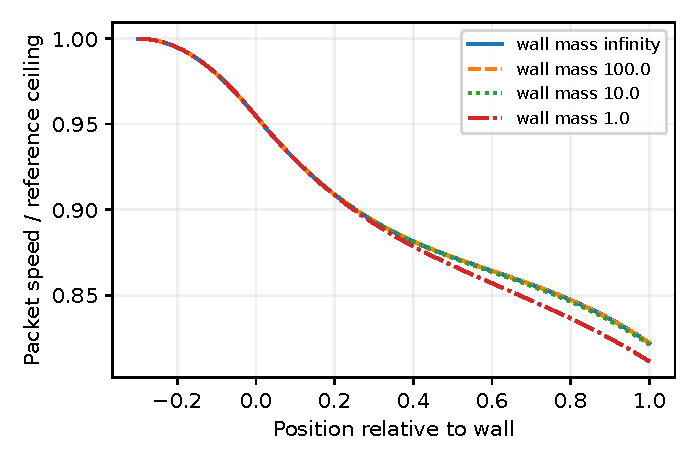
\includegraphics[width=0.96\textwidth,height=\textheight]{figures/review4_recoil.pdf}
\caption{Finite wall recoil. Packet trajectories are plotted against
position relative to the moving wall. All shown illustrative cases
arrive.}
\end{figure}

The new fixed-wall regression uses the exact velocity identity in Part
XXXI and searches each accepted dense-output interval in two
subintervals, including endpoints and wall joins. It uses bounded scalar
maximization of the analytical derivative and a 3001-point comparison
grid. This is stronger than a uniform sampling report but may miss
narrow multiple extrema and does not bound integration error rigorously.
In particular, a near-zero numerical maximum is not a sign proof. A
validated solver with interval enclosures or an analytically controlled
inequality over the complete path is the future acceptance criterion.
The static-wall instantaneous inequality and finite-capacity inequality
in Part XXXI are exact within their declared assumptions. The linear
fixed-gap solution in Part XXX provides a continuous analytic control,
with the strong-drag limiting trajectory classified as asymptotic stop
rather than arrival.

\begin{longtable}[]{@{}llr@{}}
\toprule\noalign{}
New fixed-wall case & Status & Max searched \(\dot v\) \\
\midrule\noalign{}
\endhead
\bottomrule\noalign{}
\endlastfoot
Baseline & arrived & \(-1.0000\times10^{-6}\) \\
Refined & arrived & \(-1.0000\times10^{-6}\) \\
RK45 control & arrived & \(-1.0000\times10^{-6}\) \\
No exchange & arrived & 0.331516 \\
Low capacity & arrived & 0.327398 \\
High emission energy & arrived & 0.277769 \\
Stop threshold control & stopped & see CSV \\
Short horizon control & incomplete & see CSV \\
\end{longtable}

The full 12-case new grid has ten arrivals, one momentum-threshold stop,
and one timeout deliberately produced by a shortened integration
horizon. The old 42 records are reclassified separately and all recorded
arrivals are retained; they do not count as new integrations. The
threshold stop is not a proof of permanent rest, while a timeout is not
a stop or a physical horizon. Baseline DOP853 uses relative tolerance
\(10^{-10}\), absolute tolerance \(10^{-12}\), maximum step 0.04;
refined DOP853 uses \(10^{-12}\), \(10^{-14}\), 0.01. RK45 uses
\(10^{-11}\), \(10^{-13}\), 0.02. The largest difference over arrival
time, final speed, energy and gap against the baseline is
\(1.848\times10^{-11}\); these are empirical numerical convergence
estimates, not rigorous error bounds. In the baseline the searched
maximum is at emission, with negative derivative \(-10^{-6}\); the
refined energy residual is about \(2.17\times10^{-13}\). The positive
result remains restricted to a selected physical-history ansatz.

\begin{figure}
\centering
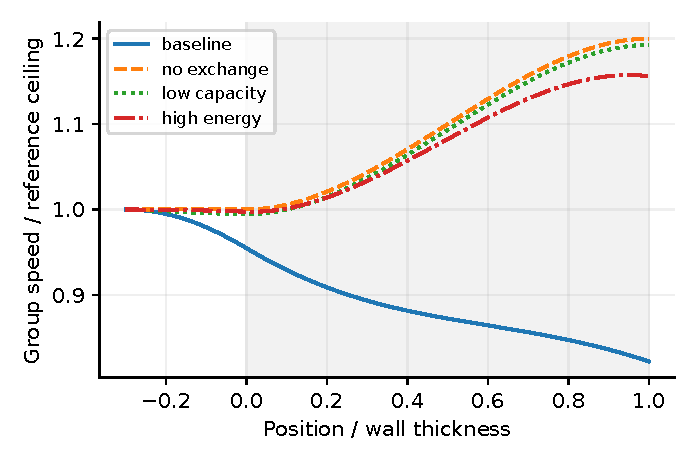
\includegraphics[width=0.96\textwidth,height=\textheight]{figures/review4_wall.pdf}
\caption{Adaptive-wall regression controls, with a selected successful
case and contrasting reacceleration cases. These are normalized toy
trajectories, not measured cosmic light speeds.}
\end{figure}

\subsection{A local gauge-consistent conversion
candidate}\label{a-local-gauge-consistent-conversion-candidate}

The one-way Part XXXI rate has not yet been derived from an underlying
local field. A constructive intermediate model is reversible conversion
between two massive-vector branches in a finite reservoir. It
distinguishes the bare reference photon mass \(m_0>0\) from a possible
dressed branch with gap \(m_1>m_0\); the second gap is an excitation
parameter, not a measured change in the invariant bare mass. This is an
effective two-mode hypothesis. Whether a single electromagnetic
excitation with local dressing realizes these branches is a separate
derivation.

For a homogeneous normalized sector set \(B=C=\hbar=1\) and use the
algebraic contraction convention \((+---)\) on the constant ordering and
spatial coordinates. Define
\(F_{i\mu\nu}=\partial_\mu A_{i\nu}-\partial_\nu A_{i\mu}\) with
antisymmetrized indices, and
\(B_{i\mu}=A_{i\mu}-m_i^{-1}\partial_\mu\theta_i\). Under
\(A_i\to A_i+\partial\Lambda_i\), \(\theta_i\to\theta_i+m_i\Lambda_i\),
\(B_i\) is invariant. Let two real massive reservoir fields
\(\phi_0,\phi_1\) have masses \(M\) and \(M+\delta\), with \(\delta>0\).
A local candidate action density is

\[\begin{aligned}
\mathcal L={}&\sum_{i=0}^1\left[-\tfrac14 F_i^{\mu\nu}F_{i\mu\nu}
+\tfrac12 m_i^2 B_i^\mu B_{i\mu}\right]\\
&+\sum_{j=0}^1\left[\tfrac12\partial_\mu\phi_j\partial^\mu\phi_j
-\tfrac12 M_j^2\phi_j^2\right]\\
&-\tfrac12 g_b\phi_0\phi_1 F_0^{\mu\nu}F_{1\mu\nu}-V_b(\phi_0,\phi_1).
\end{aligned}\tag{H3}\]

The interaction is gauge invariant, time-reversal symmetric for real
coefficients and local, and admits the process
\(\gamma_0+b_0\leftrightarrow\gamma_1+b_1\). This action is an EFT
candidate in a bounded-amplitude domain; the mixed vector kinetic matrix
is positive for \(|g_b\phi_0\phi_1|<1\) in this normalization. A bounded
mixing function or a stable microscopic completion, positive reservoir
potential, a constrained Hamiltonian including longitudinal modes, and
the full principal symbol are required before global stability or
causality is established. In the weak-mixing homogeneous control, free
fields have characteristic 1. The derivative coupling changes the full
equations in backgrounds with nonzero fields; neither hyperbolicity for
arbitrary states nor a global causal proof follows from gauge invariance
alone. No instantaneous remote reservoir is assumed. A finite physical
region requires explicit initial data and energy/momentum flux through
the boundary.

A dynamical regulator may enter the vector kinetic coefficients and
environmental mass matrix via local functions of \(I\), with its own
retarded scalar action, positive kinetic coefficient and potential. For
example
\(\mathcal L_I=(\dot I^2/C_I^2-|\nabla I|^2-\lambda^{-2}I^2)/2+gI\rho_s\)
generates the linear regulator equation in a prescribed source control.
If the vector and bath Lagrangians depend on \(I\), their
\(\partial\mathcal L/\partial I\) terms enter the regulator equation,
and the matter source must react via variation of the same action. A
time- and translation-invariant full local action has a conserved
Noether energy and momentum current including every sector; in a finite
volume the change equals the boundary flux. For the free scalar
reservoir, energy density is
\((\dot\phi^2+|\nabla\phi|^2+M_j^2\phi^2)/2\) and energy flux is
\(-\dot\phi\nabla\phi\). The interaction changes these separate
currents; only the total is conserved. This provides an explicit local
route for recoil and spatial energy transport, but we have not solved
the interacting PDE or derived the C-01 response from its microphysics.

\subsection{Exact conversion kinematics and polarization
control}\label{exact-conversion-kinematics-and-polarization-control}

With a stationary bath particle, incoming packet energy \(E\) and mass
\(m_0\), total invariant \(s=M^2+m_0^2+2ME\). The forward channel is
open when \(\sqrt{s}\geq m_1+M+\delta\). Its center-of-momentum outgoing
magnitude is

\[q_*^2=\frac{[s-(m_1+M+\delta)^2][s-(m_1-M-\delta)^2]}{4s}.\tag{H4}\]

The outgoing vector has energy \(E_*=\sqrt{m_1^2+q_*^2}\). Boost back to
the bath reference at speed \(p/(E+M)\), where \(p=\sqrt{E^2-m_0^2}\).
For scattering angle \(\theta_*\) the outgoing longitudinal component is
\(p_z'=\Gamma(q_*\cos\theta_*+bE_*)\) and transverse component
\(p_\perp'=q_*\sin\theta_*\). The target takes the missing momentum
exactly and its final energy is
\(\sqrt{(M+\delta)^2+|\mathbf{p}-\mathbf{p}'|^2}\). The increase in
target rest energy is \(\delta\), while the residual kinetic energy is
recoil. These are exact two-body consequences for the normalized
constant-coefficient model. Threshold and recoil constrain which aging
events can occur; a kinematically allowed event is not necessarily
probable.

The \(F_0F_1\) vertex produces the polarization contraction, up to an
overall coupling normalization,

\[\mathcal M\propto 2[(p\cdot p')(e\cdot e')-(p\cdot e')(p'\cdot e)].\tag{H5}\]

Replacing either polarization by its own momentum yields zero, a
gauge-consistency check on this vertex. In the exact forward collinear
control the transverse-to-longitudinal contraction vanishes; for nonzero
angle a longitudinal component can occur. This is not proof of
polarization preservation for a macroscopic beam. Differential rates
need flux factors, final phase space, physical coupling, thermal
distributions, attenuation and detector response, and all other
permitted processes. A transverse-to-longitudinal matrix-element
fraction at one angle is not an integrated branching probability.

For \(E=1\), \(m_0=10^{-6}\), \(m_1=0.5\), \(M=100\), \(\delta=0.1\),
forward scattering yields \(E'=0.8996826713\), \(v'=0.83134846\), zero
angular deflection and target recoil energy 0.00031733. At
\(\theta_*=0.1\) rad the lab angle is 5.66173 degrees, the retained
energy 0.89964611, and the longitudinal weight from the unpolarized
transverse-input contractions is 0.050386. These values are neither
observed linewidths nor cross sections. The multi-energy and multi-gap
scan contains 112 kinematic combinations, 98 allowed and 14 below
threshold; allowed cases close the energy ledger to better than
\(10^{-12}\) in normalized units. It demonstrates a possible local
channel that slows and increases effective gap without violating
conservation. It also identifies a potentially serious scattering and
polarization requirement. No frequency-independent aging law follows
from the scan.

\begin{figure}
\centering
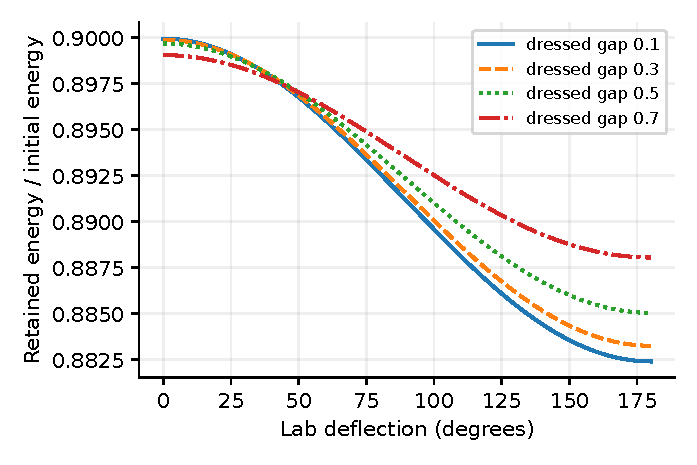
\includegraphics[width=0.96\textwidth,height=\textheight]{figures/review4_collision.pdf}
\caption{Local two-branch conversion control. Different dressed gaps
yield distinct allowed energy and deflection pairs. The curves sample
center-of-momentum angles and are not angular probabilities.}
\end{figure}

\subsection{Capacity, reverse reactions and optical
coherence}\label{capacity-reverse-reactions-and-optical-coherence}

For a finite local bath with \(N\) available sites and occupancy \(n\),
a minimal reversible rate control is \(\dot n=k_+(N-n)-k_-n\). With
constant rates the stable equilibrium is \(n_*=Nk_+/(k_++k_-)\); at
equilibrium both fluxes match. The included example \(N=10\),
\(k_+=0.4\), \(k_-=0.1\) approaches occupancy 8, not unbounded
absorption. A thermal realization must derive forward and reverse rates
from (H3), densities of states and energy/momentum conservation. For a
thermal two-state system coupled to a bath at temperature \(\Theta\),
detailed balance for fixed level energies and degeneracies fixes
\(n_*/(N-n_*)=(g_1/g_0)\exp[-\Delta E/(k_B\Theta)]\). Equivalently, the
ratio is \(\exp[-\Delta F/(k_B\Theta)]\) with
\(\Delta F=\Delta E-k_B\Theta\ln(g_1/g_0)\) under these two-level
assumptions. Do not include the degeneracy factor again if it is already
included in the free-energy difference. An imposed one-way rate is
justified only in a controlled nonequilibrium limit with an actual heat
and entropy budget. Spatial transport requires a continuity equation for
each species with transport flux and the corresponding conversion
source; reservoir fields, particle kinetics or a causal fluid closure
must supply these fluxes and recoil. Repeated packets can saturate the
bath or drive reverse emission. The simple occupancy curve is a test of
balance, not a rate prediction for cosmology.

Chapter 30S in \emph{BEYOND SPACETIME} studies emission into a scalar
branch without assuming photon gap conversion. Its selected small-gap
bath upper-speed deficit, evaluated in high precision for gap ratio
\(10^{-8}\) and final-to-initial energy ratio \(1/2\), is approximately
\(10^{-16}\) rather than \(2\times10^{-16}\). This is a roundoff
correction, not a changed physical conclusion. The branch-changing EFT
here instead introduces two vector states and two massive bath states.
Both have conservation, recoil and angular constraints, but neither is
derived from the other. The common kinematic principle is energy and
momentum balance at each local vertex. To identify the mechanisms, a
single Hamiltonian must reproduce the scalar emission channel, the
effective dressed-state pole, its self-energy and lifetime, and the
coarse-grained Part XXXI conversion coordinate and capacity. That
calculation has not been completed. They remain distinct candidates.

Spectral and directional coherence impose a stronger gate than mean
energy loss. Given a differential transition rate, compute the first and
second energy-loss moments, angular diffusion tensor, Stokes transfer
and longitudinal leakage jointly. The detector must register the line
shape, not just the total remaining energy. For a conserved current
\(J^\mu\), the interaction \(-J^\mu(d_0 A_{0\mu}+d_1 A_{1\mu})\) is
gauge invariant up to a boundary term if the couplings are constant and
\(\partial_\mu J^\mu=0\). Variable couplings require conserved effective
currents or the gauge-invariant \(B_i\) fields with an appropriate
matter model. A detector with initial rest mass \(M_d\) at rest and
final bound state mass \(M_d^*\) can absorb a branch of mass \(m_i\)
with energy \(E_i\) only when the isolated single-final-state condition
\((M_d^*)^2=M_d^2+m_i^2+2M_d E_i\) is met (normalized units); other
channels add their energy and momentum. The reverse emission has its own
recoil condition. The resonance and response weights of the dressed
branch cannot be inferred from the ordinary transverse massless
response. The source and detector must be solved with the same
electron/nuclear standards and interaction, and the resulting phase,
survival, spectral width and arrival maps fed into (O1). This is the
pending microscopic and astronomical closure, not an established
spectroscopic redshift.

\section{Relational gravity, horizons and the wider
program}\label{relational-gravity-horizons-and-the-wider-program}

The original gravity reports investigate a relational physical-force
alternative to interpreting curvature as a substance. A full theory must
reproduce solar-system light bending, Shapiro delay, orbit precession,
gravitational clock shifts, binary pulsar losses, equivalence-principle
tests and gravitational radiation. Treating Newtonian attraction or an
arbitrary Machian kernel as an all-purpose substitute does not supply
those results. The positive-mass photon proposal also requires a
consistent description of polarization, gravitational deflection and
black-hole capture. A packet horizon caused by accumulated slowing or a
particular detector trajectory is not automatically a universal
information horizon. Conventional black-hole observations involve
stellar/gas dynamics, accretion, lensing and ring structures; a proposed
capture law must predict those independently.

The dark-sector and propulsion reports (Z15, Z21, L06, L11) explore
whether massive-photon remnants or collective inertia can account for
missing gravitational effects and enable physical propulsion. They
remain a separate research branch. A loss mechanism that deposits energy
must predict where it goes, how its momentum is transferred, the
resulting equation of state, and the resulting lensing and clustering.
Galaxy rotation curves and merging clusters constrain whether that
energy can be identified with the inferred dark component. The present
packet's finite rest energy does not establish a stable population, its
density, or a workable propulsion source. Any vehicle model needs a mass
intake, force, reaction momentum and energy ledger. No propulsion
performance is established by the simulations in this review.

\subsection{Tidal-sign convention and exterior source
control}\label{tidal-sign-convention-and-exterior-source-control}

Use \(\mathbf g=-\nabla\Phi\) and define the tidal acceleration tensor
\(\mathcal T_{ij}=\partial_j g_i=-\partial_i\partial_j\Phi\). The sign
fixes the differential acceleration
\(\delta\dot v_i=\mathcal T_{ij}\delta x_j\). For \(\Phi=-GM/r\) and a
distant source in direction \(\mathbf n\),
\(\mathcal T_{ij}=(GM/D^3)(3n_in_j-\delta_{ij})\). Longitudinal
eigenvalue \(+2GM/D^3\) means stretching of physical separations; the
two transverse eigenvalues \(-GM/D^3\) mean compression. The vacuum
trace is zero, not a first-order isotropic outward force. This corrects
the inconsistent Hessian sign on historical pages 126 and 137 of the
earlier book edition while preserving the physical interpretation. The
revised main book (24 November 2026, Review 4.0 hardcover) uses the
acceleration-gradient convention on PDF pages 128 and 139. A screened
external field can have nonzero interior divergence but its sign and
magnitude must follow from its source and coupling. No shell force or
boundary is assumed as an observation.

\subsection{Retained gravitational and cosmic-domain
development}\label{retained-gravitational-and-cosmic-domain-development}

The Part XXIX gravity branch selects a retarded symmetric rank-two
interaction as a candidate physical mediator, sourced by total conserved
stress-energy. It is not yet a nonlinear theory of gravity. The
completion must handle constraints, universally coupled matter, mediator
degrees of freedom, positive energy, radiation and backreaction. Use
conventional weak-field and compact-object observables as calibration
targets without assigning material substance to coordinates. A separate
C-01 regulator may need nonlinear screening to maintain local precision
while retaining cosmic sensitivity. Derive the coupling between the
sectors instead of assuming equivalence with a conventional metric
solution.

For the photon-remnant branch, the imported energy audit is informative:
a reference present CMB number density of 410.7 per cubic centimeter and
an assumed rest-energy gap of at most \(10^{-18}\) eV imply at most
\(4.107\times10^{-16}\) eV per cubic centimeter in stopped rest energy
of that specified population. Relative to the illustrative dark-sector
density \(1264.41\) eV per cubic centimeter, this is about
\(3.25\times10^{-19}\). This is an inventory calculation for those
inputs, not a general exclusion of other physical reservoirs or
mass-generation mechanisms. A credible reservoir requires an independent
production history, energy, clustering and lensing prediction. Maintain
a momentum ledger for any proposed collection or propulsion process.

For bubble evolution, represent a wall as a physical density/stress
configuration with finite thickness and conserved material flux. Test
isolated, off-center, asymmetric, overlapping and dissolving domains. A
circle-overlap plot is only a geometry benchmark; it cannot predict
radiation or polarization without a dynamical field theory. The curated
sixth report suggests circular temperature and correlated polarization
templates as search controls, but no specific ArcSecs template or
confirmed bubble signature follows. Predeclare search parameters, masks,
foreground controls, injection/recovery thresholds and look-elsewhere
correction. Treat reported null searches as information about
sensitivity rather than evidence that a domain has been detected. No
exterior or total cosmic age is assigned from an observable boundary
alone.

\section{Part XXXIII --- Bounded local interactions and a
continuous-history
test}\label{part-xxxiii-bounded-local-interactions-and-a-continuous-history-test}

\textbf{Status of this chapter.} The independent audit is a targeted
computational and editorial review, not a physical experiment or an
exhaustive proof of the preceding manuscript. Its supplied
implementation was rerun without modifying its equations: all 21 case
classifications (arrival, incomplete, sampled reacceleration and
saturation flags) agree with the supplied records, and the selected
endpoint values agree exactly at the stored precision in this
environment. These 21 cases include refinements and negative controls,
not 21 independent observations. Two confirmed editorial corrections
have been made in the preceding sections. The following new results are
analytical consequences or executed synthetic benchmarks. The C-01
initial emission objective remains an unresolved requirement, and the
three radiation candidates remain separate.

\subsection{One local action with bounded kinetic
mixing}\label{one-local-action-with-bounded-kinetic-mixing}

Use a declared common ordering coordinate \(T\) and nonmaterial spatial
coordinates \(\mathbf{x}\). Normalize a reference fastest characteristic
and \(\hbar\) to one. This is a preferred-background effective field
model, not an assertion that geometry is a physical substance. In this
section \(B_*\) denotes the reference all-sector speed (one in
normalized units); \(\mathbf{B}_i\) denotes magnetic induction and must
not be confused with that speed or the gauge-invariant vector
\(B_{i\mu}\) of H3. Let \(I\) be a real regulator field,
\(\phi_0,\phi_1\) real massive reservoir fields, and \(\Psi_a\) complex
charged matter fields. Let \(m_i>0\) be fixed bare vector mass
parameters. Use the gauge transformations of H3 and define
\(U_{i\mu}=A_{i\mu}-\partial_\mu\theta_i/m_i\). For an illustrative
bounded branch mixing let

\[\chi=\chi_m\tanh(g_b\phi_0\phi_1/\chi_m),\qquad 0<\chi_m<1.\tag{J1}\]

Define the two-by-two electric matrix
\(K=C^{-1}\left(\begin{smallmatrix}1&\chi\\\chi&1\end{smallmatrix}\right)\)
and the diagonal mass matrix \(D=\operatorname{diag}(m_0^2,m_1^2)\). Set
\(C(I)=(1+\alpha I^2)^{-1/2}\) with \(\alpha\geq0\). The diagonal
transverse constitutive response is impedance matched in the chosen
normalized units: \(\epsilon=C^{-1}\) and \(\mu=C^{-1}\) when
\(\chi=0\). The off-diagonal response is a distinct physical
interaction. A candidate local action is \(S=\int dT\,d^3x\,\mathcal L\)
with

\[\begin{aligned}
\mathcal L={}&\mathcal L_v+\mathcal L_I+\mathcal L_b+\mathcal L_m,\\
\mathcal L_v={}&\tfrac12\mathbf E^t K\mathbf E
-\tfrac12 C^2\mathbf B^t K\mathbf B\\
&+\tfrac1{2C^2}U_0^tDU_0-\tfrac12\mathbf U^tD\mathbf U,\\
\mathcal L_I={}&\tfrac12\dot I^2-\tfrac12|\nabla I|^2-\tfrac12\mu_I^2I^2,\\
\mathcal L_b={}&\sum_j\tfrac12(\dot\phi_j^2-|\nabla\phi_j|^2
-M_j(I)^2\phi_j^2)-V_b,\\
\mathcal L_m={}&\sum_a\big[|\mathcal D_T\Psi_a|^2
-|\boldsymbol{\mathcal D}\Psi_a|^2\\
&\hspace{2em}-M_a(I)^2|\Psi_a|^2\big]-V_m.
\end{aligned}\tag{J2}\]

Here field contractions sum over vector branches and, for three-vectors,
over spatial components;
\(\mathcal D_\mu=\partial_\mu+i\sum_i q_{ai}A_{i\mu}\). The charges are
constant, and \(\Psi_a\) transforms with the compensating phase.
\(V_b,V_m\) are differentiable, nonnegative gauge-invariant potentials.
A possible test family is \(M_a(I)=M_{a0}\exp[-\kappa_a I]\) (similarly
for a reservoir mass if desired). All \(M_a,M_j\) must be positive.
Canonical field dimensions in four coordinates with reference units
\(\hbar=B_*=1\) give \([I]=[\phi]=[A]=[\Psi]=\) energy,
\([g_b]=[\alpha]=\) inverse energy squared and \([\kappa]=\) inverse
energy. The mass matrix \(D\) is independent of \(I\); the physical
excitation poles need not equal its entries. No measured coupling is
assumed. J2 is a new classical EFT candidate, not a derivation of
quantum electrodynamics or a fitted gravity theory. Its two distinct
physical vector branches are not yet evidence for a single photon
changing intrinsic mass.

The regulator equation from this \emph{same} action is

\[\begin{aligned}
(\partial_T^2-\nabla^2+\mu_I^2)I={}&\partial_I\mathcal L_v\\
&-\sum_j M_j M_j'\phi_j^2\\
&-2\sum_a M_a M_a'|\Psi_a|^2 .
\end{aligned}\tag{J3}\]

Potentials in this expression are chosen independent of \(I\); otherwise
their derivatives also enter. The bath equations similarly include
\(\partial_{\phi_j}\mathcal L_v\), \(M_j^2\phi_j\) and
\(\partial_{\phi_j}V_b\). In unitary gauge \(\theta_i=0\) the vector
equations follow from variation of \(A_{i0},\mathbf A_i\): the electric
displacement is \(K\mathbf E\), the magnetic intensity is
\(C^2K\mathbf B\), and the mass terms are \(D U_0/C^2\) and
\(D\mathbf U\). The Gauss constraint includes the matter charge
densities. For conserved matter currents the Stückelberg equations give
the divergences of the corresponding mass currents. Varying the matter
fields gives
\(\mathcal D_\mu\mathcal D^\mu\Psi_a+M_a^2\Psi_a+\partial_{\Psi_a^*}V_m=0\)
in the reference algebraic contraction. Matter current conservation
follows from the gauge-invariant action; using an arbitrary
space-dependent multiplying charge would not generally preserve it. This
is why constant branch charges, or separately derived gauge-invariant
interactions, are required.

For weak, slowly moving matter and negligible other sources, the mass
derivatives in J3 give a density source proportional to \(\kappa_a\)
times rest-energy density in the eikonal matter limit. This recovers the
earlier screened static equation as an approximation with a defined
source normalization. For prescribed homogeneous density \(\rho_s\),
\(I=g\rho_s/\mu_I^2\); the shell result of Part XXVII is its
finite-range Green-function control, not Newtonian shell acceleration. A
step in a source Fourier component \(\rho_{\mathbf k}\) gives
\(I_{\mathbf k}(T)=g\rho_{\mathbf k}(1-\cos \omega_k T)/\omega_k^2\) for
zero initial data and \(\omega_k^2=|\mathbf k|^2+\mu_I^2\). This does
not relax to the static value without damping or outward wave transport.
Fourier components describe a globally specified source, not
instantaneous distant physical response. Compact local sources propagate
through the retarded wave equation; the full interaction changes both
the source and field. Use finite-energy perturbations on a prescribed
background, or finite regions with boundary flux, rather than an
infinite total source integral. A uniform density in an unbounded domain
is finite density, not infinite density.

\subsection{Energy, constraints and characteristic
cones}\label{energy-constraints-and-characteristic-cones}

The kinetic eigenvalues of \(K\) are \((1\pm\chi)/C\), so
\(\lambda_{\min}\geq(1-\chi_m)/C\). The tanh coupling proposed by the
independent audit is a change in the local interaction, not a numerical
clamp on a trajectory. Its low-field expansion recovers H3 in the
homogeneous \(C=1\) normalization. It introduces higher-order operators
and does not establish a UV completion.

In unitary gauge let \(\mathbf\Pi\) be the canonical vector momenta,
with the conventional sign chosen according to
\(\mathbf E=-\dot{\mathbf A}-\nabla A_0\). Eliminating the nondynamical
temporal components by Gauss' equation gives an additional nonnegative
term \(C^2\mathcal G^tD^{-1}\mathcal G/2\), where \(\mathcal G\) is the
signed divergence of \(\mathbf\Pi\) plus the corresponding signed matter
charge density. Thus the reduced vector Hamiltonian contains

\[\begin{aligned}
\mathcal H_v={}&\tfrac12\mathbf\Pi^tK^{-1}\mathbf\Pi
+\tfrac12 C^2\mathbf B^tK\mathbf B\\
&+\tfrac12\mathbf A^tD\mathbf A
+\tfrac12 C^2\mathcal G^tD^{-1}\mathcal G.
\end{aligned}\tag{J4}\]

The scalar and matter Hamiltonians contain nonnegative kinetic,
gradient, mass and stipulated potential terms (with spatial covariant
derivatives for charged matter). Boundary terms must vanish or be
included. This argument is classical, for smooth finite fields, positive
\(C\) and positive masses; it does not certify vacuum stability after
quantization or finite-amplitude solutions for arbitrary data. If \(I\)
is allowed to grow without bound, \(C\) can approach zero and uniform
coercivity is lost. Restrict the effective domain to finite regulator
amplitudes until uniform lower bounds are derived. For a
translation-invariant action, total canonical energy and momentum
satisfy \(\partial_T\mathcal E+\nabla\cdot\mathbf S=0\) and
\(\partial_T\mathcal P_i+\partial_j\Pi_{ij}=0\) on solutions, with total
flux through any chosen physical boundary. Individual sectors exchange
energy and momentum. No independent source or immobile wall can be added
to the closed ledger without its work and reaction.

For a frozen homogeneous background, diagonalize the positive kinetic
matrix and the mass matrix by generalized eigenvectors. Both transverse
and longitudinal physical branches have dispersion

\[\omega_j^2=C^2 k^2+\lambda_j,\quad
\det(D-\lambda_j K)=0.\tag{J5}\]

The longitudinal expression follows from eliminating the temporal
component: the temporal mass coefficient \(D/C^2\) and spatial
coefficient \(D\) are deliberately paired, so each diagonalized
longitudinal mode has the same characteristic \(C\). In the Stückelberg
description the mass-current scalar has a principal kinetic term
proportional to \((\partial_T\theta)^2/C^2-|\nabla\theta|^2\). At a
smooth background the coefficients in J2 depend on undifferentiated
scalar fields; variations of their gradients multiply first derivatives,
not new mixed second derivatives. The frozen physical principal
characteristics are therefore \(C\) for the vector/Stückelberg sector
and one for regulator, bath and charged scalar sectors, with the gauge
and Gauss constraints enforced. This is a principal-symbol and
reduced-energy check; a global nonlinear well-posedness proof, quantized
stability, interfaces with discontinuous coefficients and
matter-dependent characteristic transformations remain to be supplied.
In particular the choice \(C(I)\) is constitutive, not a microphysical
calculation of \(c_0\). A positive bare mass does not fix the numerical
value of the characteristic speed.

\begin{figure}
\centering
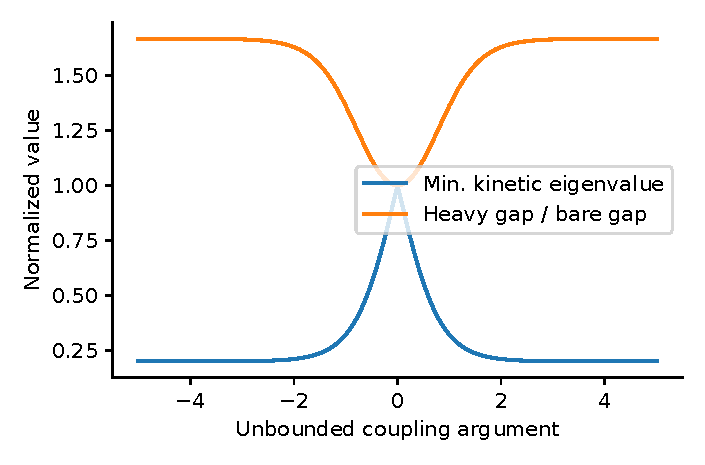
\includegraphics[width=0.96\textwidth,height=\textheight]{figures/review5_mixing.pdf}
\caption{Bounded mixing at fixed C=1. A positive lower kinetic
eigenvalue is maintained; coherent mass poles still change and remain
distinct.}
\end{figure}

At \(C=1\) let \(\ell=\lambda_j\). The two poles satisfy

\[(1-\chi^2)\ell^2-(m_0^2+m_1^2)\ell+m_0^2m_1^2=0.\tag{J6}\]

The heavier pole increases with \(|\chi|\) and the lighter pole
decreases, approaching \(m_0\) as mixing vanishes. The numerical scan
uses \(m_0=10^{-6}\), \(m_1=0.5\), \(\chi_m=0.8\) and 201 coupling
arguments between -5 and 5. The lower kinetic eigenvalue remains at
least 0.2. A stationary coherent mixing state changes the local
eigenmodes, not an irreversible record of past travel. In particular a
packet following a local pole may recover its original dispersion upon
leaving the medium. A history variable needs additional physical degrees
of freedom or a controlled loss of coherence and spatial separation of
the reservoir excitations. J6 does not derive Part XXXI's \(\Delta(a)\).

\subsection{Physical emission, recoil and detector
currents}\label{physical-emission-recoil-and-detector-currents}

For an isolated source with excited rest energy \(M_e\) and ground rest
energy \(M_g\), a homogeneous \(C=B_*=1\) emission into a vector branch
of mass \(m\) requires \(M_e\geq M_g+m\). Exact two-body recoil at rest
gives

\[ E_{\rm emit}=\frac{M_e^2-M_g^2+m^2}{2M_e},\quad
v_{\rm emit}=\sqrt{1-m^2/E_{\rm emit}^2}.\tag{J7}\]

Absorption by a ground-state receiver at rest into the single excited
state requires \(E_{\rm abs}=(M_e^2-M_g^2-m^2)/(2M_g)\). The two
energies differ by recoil; a freely recoiling receiver need not be
resonant with the source. Additional transitions, linewidths or a
recoil-sharing support can change the detector's acceptance. In the
homogeneous positive-gap control the group velocity is below the front
for any allowed finite emission energy. For \(M_g=100\), \(M_e=101\),
\(m=0.5\), \(E_{\rm emit}=0.996287\) and \(v_{\rm emit}=0.864947\); for
\(m=10^{-6}\) the group speed is within approximately
\(5.05\times10^{-13}\) of the unit front but not equal. Thus
finite-energy emission has a source-specific upper speed, but the
stipulated common exact initial ceiling is not yet derived. Defining the
source-specific value as the universal C-01 limit would change the
research objective. This no-equality result applies to the dispersion
J5, not to every possible new dispersion.

For a physical transition let \(J^\mu(k)\) be a matrix element of a
conserved current with \(\omega J^0=\mathbf k\cdot\mathbf J\). The
coupling amplitude is proportional to \(q_i\epsilon_{i\mu}^* J^\mu\),
multiplied by the branch residue and source overlap. An isolated free
charged particle of unchanged mass cannot spontaneously emit a
positive-mass vector in a homogeneous reference vacuum while conserving
four-momentum; the physical source needs an internal transition,
acceleration by other matter or a different channel. In the dipole
approximation a localized transition with dipole \(\mathbf d\) has
\(\mathbf J\) proportional to \(\omega\mathbf d\) and the continuity
relation determines \(J^0\). At \(C=1\), for
\(\epsilon_L=(k/m,\omega\hat{\mathbf k}/m)\),

\[ J\cdot\epsilon_L=-\frac{m}{\omega}J_\parallel.\tag{J8}\]

For equal current components the squared longitudinal factor relative to
a transverse component is \(m^2/\omega^2\). A tiny bare mass gives
suppression, but a large dressed gap need not. The angular pattern
depends on the dipole orientation and transition selection rules. At
nonzero mixing the source projects onto both kinetic-normalized
eigenvectors and must respect the same conserved current and recoil
constraints. No atomic bound-state wavefunctions were solved here; J7
and J8 are emission/absorption and conserved-current controls, not a
calibrated atomic spectrum. The inverse absorption process has the
conjugate matrix element with its own recoil and final-state phase
space.

\subsection{Differential local conversion: a decisive optical
constraint}\label{differential-local-conversion-a-decisive-optical-constraint}

Use the weak-field leading term of J1 in the homogeneous \(I=0\),
\(C=B_*=1\) scattering control. With distinct real bath states the
interaction is \(-g_b\phi_0\phi_1F_0\cdot F_1/2\). The external legs are
distinguishable, and the factor of two from the field-strength
contraction cancels the factor of one half. Up to a common irrelevant
phase, the tree matrix element is
\(g_b[(p\cdot p')(e\cdot e')-(p\cdot e')(p'\cdot e)]\). This fixes the
previously unspecified overall normalization of H5 for this particular
Lagrangian. The cross section is calculated at tree level, with no
unknown phenomenological angular weight.

Use center-of-momentum incident magnitude \(q_i\) and final magnitude
\(q_f\) from H4, vector energies \(E_i=\sqrt{q_i^2+m_0^2}\),
\(E_f=\sqrt{q_f^2+m_1^2}\) and \(u=\cos\theta_*\), \(h=\sqrt{1-u^2}\).
Choose polarization bases transverse in and out of the scattering plane
and longitudinal along each momentum. In this order the outgoing-row,
incoming-column amplitude matrix is

\[\frac{\mathcal M}{g_b}=\begin{pmatrix}
q_iq_f-E_iE_fu&0&m_0 E_f h\\
0&-d&0\\
-E_i m_1 h&0&-m_0 m_1 u
\end{pmatrix},\tag{J9}\]

where \(d=E_iE_f-q_iq_fu\). The stable expressions avoid large nearly
cancelling longitudinal terms at small bare mass. A direct four-vector
contraction at nondegenerate masses and Ward substitutions verify J9
numerically. For an unpolarized transverse input average over the first
two columns, not over three. The center-of-momentum differential cross
section for distinct final particles is (PDG kinematics convention)

\[\frac{d\sigma}{d\Omega_*}=\frac{q_f}{64\pi^2 s q_i}
\frac1{n_i}\sum_{a,b}|\mathcal M_{ba}|^2.\tag{J10}\]

Use \(n_i=2\) for the transverse input control or 3 for the fully
spin-averaged reciprocity test. For the reversed channel with equal spin
degeneracies and the same invariant energy, the spin-averaged amplitudes
obey \(q_i^2\sigma_{01}=q_f^2\sigma_{10}\) after integrating the reverse
angles. This is not a thermal population ratio; collision fluxes and
distributions must also be included. The tree cross section has
dimension inverse energy squared. The example \(g_b=0.01\) in normalized
inverse-energy-squared units is a chosen perturbative coupling, not a
measured coupling; cross sections here cannot be converted to cosmic
optical depths without a physical scale, density and EFT validity range.
Higher vertices, crossed channels and loop corrections are not included.
The kinematics used here are not transferable unchanged to a general
\(I\neq0\) background whose sectors have different characteristics.

For a stationary target of mass \(M=100\), final target mass \(100.1\),
\(m_0=10^{-6}\) and \(m_1=0.5\), the threshold incident energy is
\(0.6018\). At \(E=1\) the integrated transverse-input cross section is
\(1.39636614\times10^{-10}\) in the chosen units. Integrate over \(u\)
with 128-point Gauss-Legendre quadrature and repeat with 256 points. In
the target rest frame use the exact boost given in H4; the outgoing
longitudinal weight must be projected onto the lab basis, since for a
massive vector this decomposition can differ from the CM basis. The
polarization-summed transverse-input squared amplitude agrees under the
boost. The following results are conditional on \textbf{one conversion};
no conversion probability over a cosmic path has been inferred.

\begin{longtable}[]{@{}lr@{}}
\toprule\noalign{}
Quantity & Value at E=1 \\
\midrule\noalign{}
\endhead
\bottomrule\noalign{}
\endlastfoot
Mean retained energy & 0.889076 \\
Energy standard deviation & 0.0031133 \\
Mean lab deflection (degrees) & 119.821 \\
Mean lab directional cosine & -0.442003 \\
CM longitudinal fraction & 0.085180 \\
Lab longitudinal fraction & 0.086880 \\
Mean target recoil energy & 0.0109241 \\
Fraction inside 1 arcsec lab cone & \(1.44456\times10^{-13}\) \\
\end{longtable}

The sum of mean output energy, target rest-energy increment and mean
recoil equals the incident energy. A narrow cone fraction is integrated
directly over its small CM solid angle, not estimated by counting a
handful of random draws. Five open-channel energies (0.61, 0.75, 1, 2,
4) are included in the scan; 0.5 is below threshold. The lab angle
varies with the incident energy and threshold. In this example the
simple contact vertex heavily weights backward and large-angle
scattering. Forward events are allowed but extremely rare in the
one-arcsecond illustrative aperture. This is not a measured astronomical
resolution bound. The energy spread and longitudinal fraction also
matter; a spectrum cannot be modeled only by its mean retained energy.
This is a \textbf{negative optical-coherence result for this specific
vertex and parameter set}. It rules out adopting this benchmark as a
beam-preserving sole cosmological aging mechanism without a physically
different forward/coherent interaction. It does not retire the broader
local massive-vector research branch.

\begin{figure}
\centering
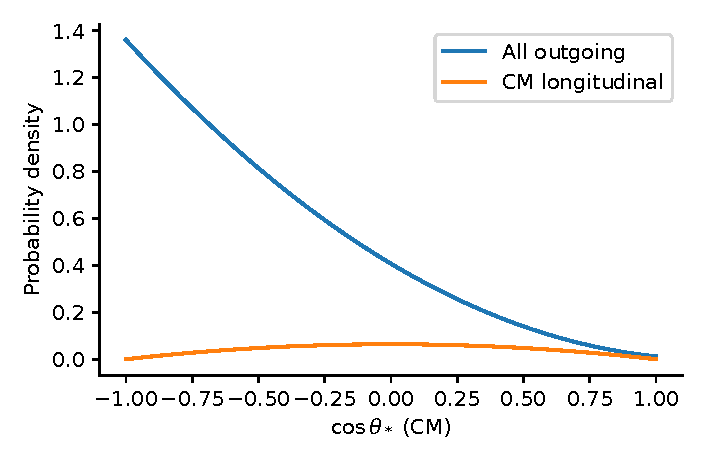
\includegraphics[width=0.96\textwidth,height=\textheight]{figures/review5_scattering.pdf}
\caption{Normalized differential conversion probability at incident
energy one. The longitudinal projection is in the center-of-momentum
basis. The curve is not a probability distribution for unconverted
photons.}
\end{figure}

A useful exact result is independent of the coupling: if a homogeneous
target starts at rest, its outgoing rest mass is larger and its kinetic
energy nonnegative, so \(E'<E\). If also \(m_1>m_0>0\), then
\(m_1/E'>m_0/E\) and \(v'<v\) in this target frame for every allowed
forward reaction, not just sampled angles. Between isolated collisions
on a fixed homogeneous background the speed is constant. Reverse
reactions, moving targets and varying \(C\) invalidate an unconditional
monotonicity claim. A sequence of forward conversions alone would
eventually stop at a threshold or exhaust the reservoir. This exact
eventwise result cannot be identified with a continuous differentiable
aging law or its absence of reacceleration in every common frame.

\subsection{Reversible finite capacity and a coarse-graining
gate}\label{reversible-finite-capacity-and-a-coarse-graining-gate}

Let the populations of two vector branches be \(f_0,f_1\) and of bath
states \(b_0,b_1\) in classical dilute phase space. The forward
collision integral has invariant measure \(d\Pi=d^3p/[(2\pi)^3 2E]\),
the kernel \((2\pi)^4\delta^4(p+k-p'-k')|\mathcal M|^2\), and occupation
difference \(f_0 b_0-f_1 b_1\) (with all arguments and polarization
labels at the matching momenta). A conventional Boltzmann equation for
\(f_0\) has the negative of this difference integrated over its partners
with the external factor \(1/(2E)\) if using
\(\partial_T+\mathbf v\cdot\nabla\) on the left; the other species use
the corresponding gain/loss permutations. Quantum statistics require the
correct Bose factors and quantum coherence treatment. The measure and
normalization stated here apply to the common unit-characteristic dilute
control. Summed collision integrals weighted by energy and momentum
vanish by the delta function. Transport carries the converted bath
states away at their own velocities; a finite domain must include those
fluxes and inflows. A local bath state is not a globally accessible
sink.

For common-temperature Maxwell-Boltzmann distributions, the occupation
difference vanishes pointwise on the energy-conserving surface if
\(\mu_{f0}+\mu_{b0}=\mu_{f1}+\mu_{b1}\), where \(\mu\) denotes chemical
potential here. This is microscopic detailed balance, rather than
one-way friction. The classical entropy production integrand is
proportional to \((X-Y)\ln(X/Y)\geq0\) with \(X=f_0b_0\), \(Y=f_1b_1\).
This statement assumes the dilute molecular-chaos approximation, a
reversible collision kernel and consistent state counting; it does not
contradict reversible microscopic evolution. For fixed two-level
energies the degeneracy convention corrected in Section 12 applies. A
genuinely irreversible effective history requires a nonequilibrium
preparation and an account of entropy, spatial transport and reverse
channels.

To isolate finite capacity we execute a deliberately restricted
pair-cell kinetic control. At one invariant energy the incident and
outgoing counterstreaming pairs have known CM flux factors
\(v_{\rm rel}=q(1/E_{\rm vec}+1/E_{\rm bath})\). Use
\(k_f=\sigma_{01}v_{{\rm rel},i}\) and
\(k_r=\sigma_{10}v_{{\rm rel},f}\) with all three initial spin states
averaged. This is a fixed-invariant-energy, randomized-spin mean-field
cell, not the full angular/thermal Boltzmann integral. Holding the mode
bins and encounter geometry fixed is an additional approximation. For
radiation density \(N\), bath density \(R\), and converted density
\(n\), the reaction counts give

\[\dot n=k_f(N-n)(R-n)-k_r n^2.\tag{J11}\]

Rescale time by \(k_f\) times the chosen density unit. Both rates come
from J10 for the chosen pair cell, with ratio \(k_r/k_f=1.48512724\).
Forward and reverse counts conserve each species total and conserve pair
energy and momentum in each microscopic event. The density closure
tracks populations, not spatial momentum distributions; its moment
closure is not a proof of a closed dynamical radiation fluid. The
physical time scale is undetermined until the density and coupling units
are assigned. At \(n=0\) the derivative is nonnegative; at
\(n=\min(N,R)\) it is nonpositive. The reaction difference decreases
strictly through its unique interior equilibrium for positive rates and
populations. Integrations start at both endpoints for \(N=1\) and
\(R=0.25,1,4\); they approach the same equilibrium in each pair of runs.
For \(R=0.25\), \(n_*=0.186501\). A reverse-prepared cell produces
\emph{more} light-branch radiation, contrary to unconditional monotonic
aging. Saturation and reverse flux are essential rather than numerical
corrections.

\begin{figure}
\centering
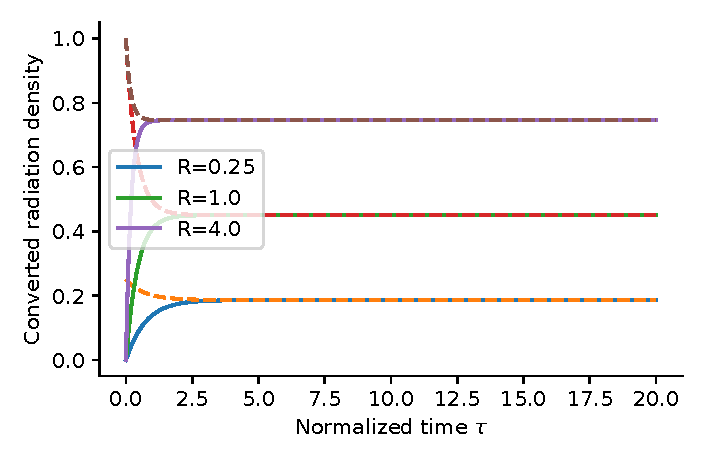
\includegraphics[width=0.96\textwidth,height=\textheight]{figures/review5_capacity.pdf}
\caption{Finite pair-cell population control. Solid curves start
unconverted; dashed curves start at maximum occupancy. They approach
common equilibria for each reservoir size. Time is normalized, not
astronomical.}
\end{figure}

The mean mass-gap-squared proxy in a two-branch mixture is
\(\overline{m^2}=(1-f)m_0^2+f m_1^2\) with converted fraction \(f=n/N\)
for fixed \(N\). It increases when forward conversion dominates and
decreases under reverse conversion. This is an ensemble moment,
\textbf{not the pole of a single radiation state}. Taking
\(\Delta=\sqrt{\overline{m^2}}\) and putting it into a single-packet
Hamiltonian is not justified: the actual distribution has at least two
mode energies, momenta and detector weights. A derivation of a
continuous history coordinate would require a dense ladder of local
dressed states or a controlled self-energy spectral pole, with drift,
diffusion, linewidth and capacity computed from the same interactions. A
small-step expansion of a jump kernel would yield first and second
moments \(A_a=\int da' (a'-a)W(a\to a')\) and
\(D_a=\int da'(a'-a)^2W(a\to a')\), not a freely chosen monotonicity
rate. Vanishing diffusion relative to the physical drift must be
demonstrated rather than assumed. J1--J11 provide no such limit for the
large discrete gap jump. Keep the Chapter 30S scalar-emission bath, Part
XXXI continuous gap-history model and Part XXXII/XXXIII vector
conversion distinct. The next microscopic gate is a forward-peaked or
coherent interaction with a derived ladder/pole, and a detector that
actually couples to it, not arbitrary suppression of scattering angles.

\subsection{Continuous monotonicity certificate for the static Part XXXI
reference}\label{continuous-monotonicity-certificate-for-the-static-part-xxxi-reference}

The prior successful numerical trajectory used a smooth static wall with
\(C=1+0.2(3x^2-2x^3)\) on \(0\leq x\leq1\), a flat lead of length 0.3,
\(E_0=1\), \(\Delta_0=10^{-6}\), capacity 2, \(\beta=K=1\) and receiver
mass 100. No wall recoil is included in this certificate. The reported
reference velocity remains 0.822103826 at arrival. Review 4.0 used
sampled/adaptive extrema and solver refinement; those checks did not
prove the continuous sign. We now enclose a different spatial
formulation on every interval, using interval arithmetic rather than
only trajectory samples.

With positive momentum define \(r=Cp\), \(b=r+Ca\), \(d=\Delta_0+a\) and
\(E=\sqrt{r^2+d^2}\). The symbol \(b\) in this subsection is a spatial
comparison variable, not a reservoir field or boost. The exact Part XXXI
equations give \(dr/dx=-C\,da/dx\) and hence

\[\begin{aligned}
\frac{db}{dx}&=C'a,\\
\frac{da}{dx}&=\left[1-\frac{d}{Cr}-\frac{aE}{100Cr}\right]_+
\left[1-\frac{a}{2}\right]_+,
\end{aligned}\tag{J12}\]

where \(r=b-Ca\). This change of independent variable is permissible if
\(v=Cr/E\) remains positive, which is verified in the enclosure. The
time derivative used for the test is the original identity

\[\dot v=\frac{v^2 C'}{C}-\frac{C^2d(d+p)}{E^3}\dot a.\tag{J13}\]

On the nonnegative branch with \(r>0\) and \(a<2\), J12 is cooperative:
\(b'\) is nondecreasing in \(a\) since \(C'\geq0\), and \(a'\) is
nondecreasing in \(b\) because \(d/r\) and \(E/r=\sqrt{1+(d/r)^2}\)
decrease as \(r\) increases at fixed \(a\). The positive-part functions
preserve these off-diagonal inequalities. Solutions from the lower and
upper corners of a state rectangle therefore bound the true solution
componentwise while remaining in the stated domain. This comparison
avoids the large interval wrapping of the initial direct \((r,a)\)
attempt (which failed to certify the sign even when refined).

For each interval of length \(h\), use trial box
\([b,b+2h]\times[a,a+2h]\) in interval notation (including the initial
uncertainty). Check the spatial derivatives lie in \([0,2)\) throughout
the box. Nonnegative derivatives prevent exit through the lower faces;
strict upper bounds prevent exit through the upper faces by integration.
Positivity of \(r,d,v\), and \(a<2\), are checked on the whole box.
Propagate the two initial corners using the interval integral enclosure
\(y(x+h)\in y(x)+h F(X,\mathcal B)\) with \(X\) the complete position
interval and each corner's own trial box; comparison then bounds the
endpoint rectangle. Evaluate J13 on the entire enclosing box. The flat
lead has \(C'=0\) and a nonpositive derivative analytically. Both joins
have continuous \(C,C'\) for this wall, so no derivative jump is
omitted. This yields an interval-comparison certificate conditional on
the stated equations and interval library's outward arithmetic, not a
formally machine-verified theorem for every model.

\begin{longtable}[]{@{}
  >{\raggedright\arraybackslash}p{(\columnwidth - 6\tabcolsep) * \real{0.2500}}
  >{\raggedleft\arraybackslash}p{(\columnwidth - 6\tabcolsep) * \real{0.2500}}
  >{\raggedleft\arraybackslash}p{(\columnwidth - 6\tabcolsep) * \real{0.2500}}
  >{\raggedleft\arraybackslash}p{(\columnwidth - 6\tabcolsep) * \real{0.2500}}@{}}
\toprule\noalign{}
\begin{minipage}[b]{\linewidth}\raggedright
Position step
\end{minipage} & \begin{minipage}[b]{\linewidth}\raggedleft
Intervals
\end{minipage} & \begin{minipage}[b]{\linewidth}\raggedleft
Wall upper bound on \(\dot v\)
\end{minipage} & \begin{minipage}[b]{\linewidth}\raggedleft
Path lower bound on \(v\)
\end{minipage} \\
\midrule\noalign{}
\endhead
\bottomrule\noalign{}
\endlastfoot
0.001 & 1300 & -0.04010 & 0.80809 \\
0.0005 & 2600 & -0.05341 & 0.81507 \\
\end{longtable}

The bounds in the table are rounded conservatively (upper toward
positive, lower downward). The fine enclosure gives
\(0.50548929\leq a_{\rm exit}\leq0.50705284\) and
\(0.47539650\leq r_{\rm exit}\leq0.47793653\) (outward rounded). The
derivative bound strictly excludes positive values throughout the rising
wall; the lead sign is nonpositive. The packet reaches the exit because
its speed remains bounded away from zero along the entire spatial path.
The code uses 40-decimal-place mpmath interval arithmetic; it reports
exact interval strings and sampled enclosure endpoints, not just the
point solver. The non-smooth positive-part rate is locally Lipschitz, so
the containment/comparison argument also covers switching surfaces in
this parameter case. This advances the continuous verification
requirement for one reduced model only. It does not establish
all-frequency, moving-wall, microscopic or astronomical monotonicity.
Independent formal interval verification would further strengthen the
numerical certificate.

\subsection{Common matter and clock
calibration}\label{common-matter-and-clock-calibration}

For a matter wave in a slowly varying regulator, the leading scalar
eikonal Hamiltonian from J2 is \(H_a=\sqrt{|\mathbf p|^2+M_a(I)^2}\) in
the common reference normalization. Hamilton's equations yield
\(\dot{\mathbf x}=\mathbf p/H_a\),
\(\dot{\mathbf p}=-M_aM_a'\nabla I/H_a\) in the absence of gauge forces;
charged matter also experiences its gauge forces. The explicit time
dependence exchanges energy with J3; the closed system conserves the
total, not the individual particle energy. This supplies a local
candidate matter force and a bounded speed without a clamp. It does not
derive a homogeneous cosmic recession law, a pressure-supported bubble
wall or an observed gravity law. A physical wall must be a solution of
coupled matter/regulator dynamics with stresses and radiation flux, not
a prescribed profile in a closed universe. The bounded ballistic
congruence of Review 4 remains a separate causal control. A total matter
separation rate may exceed a characteristic even when every local signal
lies below it.

At fixed electric charge and reference \(\hbar\), the diagonal Coulomb
strength in the unmixed regime is \(q^2/(4\pi\epsilon)=q^2C/(4\pi)\)
(provided the vector screening length is much larger than the atom). A
nonrelativistic hydrogenic transition with reduced mass \(\mu_e\) scales
as \(\nu_{\rm opt}\propto\mu_e C^2\) for fixed charges and dimensionless
level factors. Therefore

\[\delta\ln\nu_{\rm opt}=\delta\ln\mu_e+2\delta\ln C.\tag{J14}\]

With constituent masses \(M_e,M_N\) and \(\mu_e=M_eM_N/(M_e+M_N)\), the
logarithmic variation is the weighted sum

\[\begin{aligned}
\delta\ln\mu_e={}&\frac{M_N}{M_e+M_N}\delta\ln M_e\\
&+\frac{M_e}{M_e+M_N}\delta\ln M_N.
\end{aligned}\]

The example mass functions in J2 permit an explicit regulator
sensitivity but do not justify choosing it to cancel the optical shift.
Magnetic dipole/hyperfine couplings also involve permeability,
constituent moments, wavefunction density and spin structure; a nuclear
transition depends on strong-interaction parameters and nuclear
many-body states not present in the charged scalar model. J2 therefore
cannot yet predict Sr optical, Th nuclear or muon decay responses from a
common set of parameters. In the actual theory the electron spinor,
nuclear interaction and their gauge currents must replace the scalar
matter control. The dimensionless clock ratio response is the difference
of the two transition sensitivities and is observable independent of a
common clock-unit rescaling. No calibration is claimed beyond the
hydrogenic control. For emission and detection, J7 and J8 must be joined
to these physical standards and the source/detector response matrix
before a packet energy is called a spectral redshift.

\subsection{A finite-aperture 3D forward transport
control}\label{a-finite-aperture-3d-forward-transport-control}

Extend the optical ledger of Review 4 by following a converted ray in an
explicit physical geometry. A central incident ray travels along the
\(z\) axis from source to circular receiving disk at \(z=L\). One thin
conversion cell lies at \(z=d\) with \(0<d<L\), at which the incident
packet converts according to J10. Azimuth is uniform for
transverse-unpolarized input. After conversion at lab angle
\(\vartheta\), the ray intersects the receiving plane only for
\(\cos\vartheta>0\), at transverse distance \((L-d)\tan\vartheta\). If
disk radius is \(R_d\), acceptance is
\(\vartheta\leq\arctan(R_d/(L-d))\). The ray's physical path and arrival
time are distinct:

\[\begin{aligned}
\ell_{\rm path}&=d+(L-d)/\cos\vartheta,\\
T_a-T_e&=d/v_i+(L-d)/(v_f\cos\vartheta).
\end{aligned}\tag{J15}\]

This is a three-dimensional ray-direction and aperture control for one
incident central ray, not a full finite-source lensing Jacobi map or a
luminosity distance prediction. The solid-angle conversion probability
comes from J10, not a fitted attenuation. With \(L=1\), \(d=0.2\) and
the one-arcsecond illustrative aperture the conditional accepted energy
is about 0.899683, path length differs from one by less than
\(5\times10^{-12}\) and mean arrival is 1.162292 rather than direct
arrival near one. The geometric acceptance is only
\(1.44456\times10^{-13}\) of converted packets. At 0.1 rad it rises to
\(6.29316\times10^{-5}\) and mean arrival is 1.164732. Other positions
\(d=0.5,0.8\) are included. The acceptance is conditional on conversion,
the detector is idealized and the actual quantum efficiency of the
dressed branch remains unknown. Unconverted packets form a direct
component; a scattered component produces a broad distribution of
directions, energies and delays. A detector records their mixture
weighted by aperture, survival and branch-dependent absorption, not a
single shifted line. Neither the angular-size distance nor source
luminosity can be inferred from J15 alone. The earlier calibrated
brightness ledger must be applied to full ray bundles with the proper
directional area and clock ratios, including these losses; no arbitrary
compression is introduced.

For Foundation 12 the distance correction must first preserve measured
geometric anchors. Two literature checks confirm the previously reported
anchor values: the LMC eclipsing-binary distance \(49.59\) kpc
(statistical 0.09, systematic 0.54 kpc) and NGC 4258 maser distance
\(7.576\) Mpc (statistical 0.082, systematic 0.076 Mpc). These are
results of specific geometric inference procedures, not absolute
constraints independent of all matter physics. As a conditional
arithmetic control only, combining each anchor's quoted statistical and
systematic uncertainties in quadrature, a 5 percent downward shift with
unchanged calibration is about 4.53 standard-error units for the LMC and
3.39 for NGC 4258; a 20 percent shift is 18.12 and 13.55 respectively.
These are not a joint significance or an observational likelihood;
systematic errors may be correlated and a new model may change the
underlying instrument response. The raw binary, maser and Gaia data must
be jointly fitted with a dynamical calibration before assigning new
distances to the seven extreme-object dossiers. No smaller or closer
astronomical object has been independently established by this chapter.
The relevant new insight is that a physical conversion mechanism must
satisfy flux and aperture constraints as well as timing and energy
conservation.

\subsection{Development decisions and next acceptance
gates}\label{development-decisions-and-next-acceptance-gates}

Retain J1--J4 as a candidate classical bounded local action, J5--J10 as
homogeneous mode, current and scattering controls, and J12--J13 as a
continuous sign certificate for the original static reference
trajectory. The simple contact vertex tested here fails the narrow-beam
requirement in the reference parameter set. Do not use it as a completed
cosmic redshift mechanism. J11 is a reversible finite pair-cell closure,
not the Part XXXI rate. The three candidates keep distinct identities
until a genuine microscopic limit connects them. Exact finite-energy
emission at the common characteristic, a quantitative nuclear and
particle clock model, common-frame monotonicity across arbitrary
environments, fully interacting matter/field backreaction, a
dense/coherent history channel, and a held-out joint astronomical
likelihood remain open. The next investigation should derive and compare
a physically forward-peaked or coherent local conversion kernel with a
controlled pole and linewidth; couple it to conserved charged
bound-state currents and to the regulator's dynamical response before
cosmological calibration. The charter is unchanged, and no experimental
confirmation is asserted.

\section{Part XXXIV --- Forward-coherent physical conversion and the
escape
criterion}\label{part-xxxiv-forward-coherent-physical-conversion-and-the-escape-criterion}

\textbf{Research status.} This chapter extends Parts XXXII--XXXIII
rather than replacing the successful reduced Part XXXI reference. It
develops two distinct local interaction controls and a selected-mode
escape model. All new computations use normalized homogeneous units
\(C=B_*=\hbar=1\), except when a different reservoir characteristic is
explicitly declared. No measured astrophysical density, coupling,
coherence length or photon mass is inferred. The twelve foundations and
C-01 objective are unchanged. The code and tables reproduce the declared
controls, not the universe.

\subsection{A finite-range physical mediator instead of an angular
filter}\label{a-finite-range-physical-mediator-instead-of-an-angular-filter}

Extend the bounded classical action J2 by a real mediator \(\sigma\)
with positive canonical kinetic term, characteristic one in the
reference scattering calculation, and mass \(\mu_s>0\). Replace J1 for
this candidate by

\[\chi(\sigma)=\chi_m\tanh(g_s\sigma/\chi_m).\tag{K1}\]

Keep the two Stückelberg vector mass terms and the positive electric and
magnetic kinetic matrices of J2. The scalar potential can be chosen as

\[\begin{aligned}
V={}&\frac{\mu_s^2}{2}\left(\sigma+\frac{h_s}{\mu_s^2}\phi_0\phi_1\right)^2\\
&+\frac{M_0^2}{2}\phi_0^2+\frac{M_1^2}{2}\phi_1^2+V_+,\quad V_+\geq0.
\end{aligned}\tag{K2}\]

This generates the cubic vertex \(-h_s\sigma\phi_0\phi_1\) in the
Lagrangian and a nonnegative quartic completion. The field-strength term
generates \(-g_s\sigma F_0^{\mu\nu}F_{1\mu\nu}/2\) to leading order at
\(C=1\). Both couplings are local and gauge invariant. In natural units
\([g_s]=E^{-1}\), \([h_s]=E\), \([\mu_s]=E\). The electric matrix has
eigenvalues \((1\pm\chi)/C>0\) and the mass matrix is positive. The
scalar kinetic and potential energies are nonnegative; variation
supplies reciprocal sources, rather than applying a photon speed clamp.
For the frozen homogeneous background of this calculation, all principal
characteristics have the reference speed one; the scalar-sector speed
may be varied separately in a different medium. This is a classical EFT
control. It does not establish a UV-complete quantum theory, global
well-posedness of every background, or an astrophysically viable
coupling. A light mediator with fixed \(h_s\) can make the quartic term
large; the zero-mass propagator limit below is a bound on a tree-level
kernel, not a claim that K2 has a regular massless limit at fixed
couplings.

For on-shell scattering \(A+R_0\to B+R_1\) (the reservoir is initially
at rest in the lab), the tree-level exchange replaces the J9 contact
coefficient by

\[g_b\longrightarrow \frac{g_s h_s}{\mu_s^2-t},\quad t=(p-p')^2.\tag{K3}\]

The Lorentz-algebra contraction is valid here because all frozen
characteristics are one. It does not prescribe a material geometry. Its
vector tensor is still the gauge-invariant J9 tensor, so Ward
substitutions vanish. The heavy-mediator limit with \(g_s h_s/\mu_s^2\)
held fixed reproduces the contact shape and normalization. The mass scan
holds \(g_s h_s=0.01\) fixed to compare shapes; no physical
weak-coupling or unitarity bound is inferred from the formal cross
sections. In particular, large elastic cross sections in the extreme
long-range limit require an infrared/finite-size and higher-order
treatment.

\subsection{Exact forward-transfer floor for inelastic
conversion}\label{exact-forward-transfer-floor-for-inelastic-conversion}

In the center-of-momentum frame let \(q_i,q_f\) be the incoming/outgoing
vector momentum magnitudes, and \(e_i,e_f\) their energies. Put
\(y=1-\cos\theta_*\), \(b=2q_iq_f\). Then

\[\begin{aligned}
t(y)&=t_0-by,\\
t_0&=(e_i-e_f)^2-(q_i-q_f)^2,\\
a&=\mu_s^2-t_0.
\end{aligned}\tag{K4}\]

If both outgoing invariant masses exceed the respective incoming masses,
the transfer is necessarily spacelike: if \(q=p-p'\) were future causal,
\(p=p'+q\) would imply \(m_i\geq m_f\), contrary to the assumed
increase. If \(q\) were past causal, \(R_0=R_1-q\) would similarly imply
\(M_i\geq M_f\). This uses the reverse triangle inequality for future
causal momenta. Thus \(t_0<0\) even in the exactly forward direction.
Decreasing the mediator mass cannot remove the finite inelastic
momentum-transfer floor. This result does not exclude other physical
channels or near-degenerate multi-step transitions.

For incident transverse polarization averaged over its two states,
define \(d_0=e_ie_f-q_iq_f\). The positive polarization-summed tensor
weight is

\[\begin{aligned}
W(y)=\frac12\big[&(-d_0+e_ie_f y)^2\\
&+(d_0+q_iq_f y)^2\\
&+e_i^2m_f^2 y(2-y)\big].
\end{aligned}\tag{K5}\]

The differential cross section integrated over azimuth is

\[\frac{d\sigma_T}{dy}=\frac{q_f}{32\pi s q_i}
\frac{(g_sh_s)^2 W(y)}{(a+by)^2}.\tag{K6}\]

Here \(s\) is the two-body invariant squared total energy, not a
reservoir characteristic. The lab angle is computed by the exact boost
of the outgoing momentum, not identified with the center-of-momentum
angle. The normalized cone fraction uses the exact lab angle cutoff and
integrates K6. At fixed kinematics, the relative shape for larger \(a\)
compared with smaller \(a\) is proportional to
\([(a_{\rm small}+by)/(a_{\rm large}+by)]^2\), increasing in \(y\).
Consequently the normalized distribution moves toward larger angles as
\(a\) increases; the smallest possible \(a\) gives the largest forward
cone fraction within this kernel family. This is an ordering of
conditional distributions, not an absolute reaction-rate bound.

The numerical integrals use \(z=\ln(1+by/a)\) to resolve a tiny forward
cone; \(dy/(a+by)^2=e^{-z}dz/(ab)\). The forward invariant is computed
at 65 decimal digits before float quadrature. For the exact reference of
J10 (\(m_i=10^{-6}\), \(m_f=0.5\), \(M_i=100\), \(M_f=100.1\),
\(E_i=1\)), \(t_0=-0.0534657349453\) and \(\sqrt{-t_0}=0.231226587886\).
Results for a conversion event:

\begin{longtable}[]{@{}lrr@{}}
\toprule\noalign{}
Quantity & Contact J10 & Zero-mass kernel limit \\
\midrule\noalign{}
\endhead
\bottomrule\noalign{}
\endlastfoot
One-arcsec fraction & \(1.445\,10^{-13}\) & \(9.325\,10^{-11}\) \\
Mean angle (degrees) & 119.821 & 63.649 \\
Mean energy & 0.889076 & 0.894892 \\
Energy SD & 0.003113 & 0.004534 \\
Lab longitudinal fraction & 0.086880 & 0.239755 \\
\end{longtable}

Although the mediator improves the reference cone fraction by about 646
times, its absolute value is still much less than one. It also increases
the outgoing longitudinal fraction in this reference. The exact forward
kinematic energy is 0.899683 and its group speed 0.831348. No arbitrary
angular cut has been applied to the physical rate.

\begin{figure}
\centering
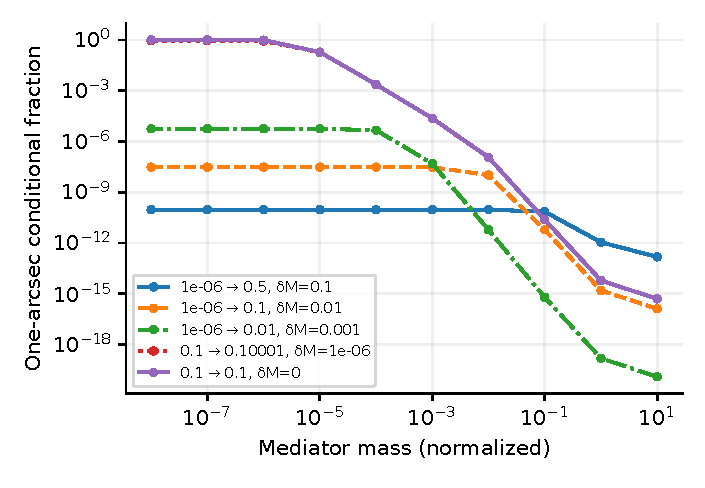
\includegraphics[width=0.9\textwidth,height=\textheight]{figures/review6_mediator.pdf}
\caption{Conditional one-arcsecond cone acceptance for seven scanned
mass combinations; five displayed. The nearly degenerate and elastic
controls can be forward-peaked, unlike the large gap change. These are
tree-level shapes, not physical astronomical cross sections.}
\end{figure}

The 72 rows include 70 positive-mass mediator cases, one contact control
and one formal massless inelastic kernel. For the near-degenerate
example \(m_i=0.1,m_f=0.10001,M_f-M_i=10^{-6}\) and \(\mu_s=10^{-8}\),
the cone fraction is approximately 0.8844, but the retained mean energy
is 0.9999989997 and the change of gap is minute. The exactly elastic
small-mediator control can approach unity cone fraction while
transferring negligible energy. These examples establish why a proposed
dense conversion ladder must be tested for cumulative angular diffusion
and optical depth, rather than assuming that each step is harmless. Even
for independent small deflections with zero mean transverse direction,
the mean-square deflection grows as the sum of the single-step variances
in the paraxial limit. An individual cone acceptance is not a bound on
the final image, and the elastic control is not photon aging. The
near-degenerate/elastic results are conditional on the Born
approximation; actual multiple scattering, screening, finite density,
perturbative unitarity and polarization transport remain unsolved.

\subsection{A phase-matched collective reservoir: collinear conversion
is
possible}\label{a-phase-matched-collective-reservoir-collinear-conversion-is-possible}

A distinct coherent control is obtained by retaining the local
interaction K1 but allowing the real physical reservoir excitation
\(\sigma\) to have a slower characteristic \(s_b\) in a material rest
frame, with dispersion \(\omega_b(Q)=\sqrt{s_b^2 Q^2+\mu_b^2}\). A
positive local kinetic term
\([\dot\sigma^2-s_b^2|\nabla\sigma|^2-\mu_b^2\sigma^2]/2\) gives this
free dispersion. It has no negative energy or super-ceiling
characteristic in the frozen background for \(0<s_b<1\). It is not the
same parameter set used to derive K6. The bounded mixing with \(\sigma\)
allows a leading \(A\to B+\sigma\) vertex; two distinct positive-mass
vector branches are retained. The reservoir must actually have the
selected excitation and a physical means to accept and transport its
momentum. This 1-to-2 conversion is a local candidate distinct from both
the 2-to-2 exchange and the Chapter 30S same-branch scalar bath.

For co-directed incident and outgoing packets in a homogeneous medium,
impose

\[\begin{aligned}
p_B&=p_A-Q>0,\\
E_A&=\sqrt{p_A^2+m_A^2},\\
E_A&=\sqrt{(p_A-Q)^2+m_B^2}+\omega_b(Q).
\end{aligned}\tag{K7}\]

For \(m_B>m_A\) and \(E_B<E_A\), \(Q> E_A-E_B\) in these units: the
momentum difference between fixed-mass states is greater than the energy
difference since \(dE/dp<1\), and increasing the final mass decreases
its momentum further at a given energy. Thus the emitted reservoir
excitation must be capable of carrying more momentum than energy in
reference units. A subcharacteristic material excitation can meet that
demand, unlike a freely propagating massive scalar with the same
reference characteristic. This is a kinematic necessity for this
collinear free-mode channel, not a proof of the existence of the
physical medium.

Choose \(m_A=10^{-6}\), \(m_B=0.5\), \(E_A=1\), \(s_b=0.4\),
\(\mu_b=0.02\). Solving K7 for a forward root gives:

\begin{longtable}[]{@{}lr@{}}
\toprule\noalign{}
Variable & Normalized value \\
\midrule\noalign{}
\endhead
\bottomrule\noalign{}
\endlastfoot
Incident momentum & 0.9999999999995 \\
Reservoir momentum \(Q\) & 0.257685206948 \\
Outgoing momentum & 0.742314793051 \\
Reservoir energy & 0.104996507279 \\
Outgoing energy & 0.895003492721 \\
Outgoing group speed & 0.829398766696 \\
Reservoir group speed & 0.392676234478 \\
\end{longtable}

The energy and momentum identities are checked to \(2\,10^{-15}\) in the
normalized calculation. The outgoing packet is slower, retains a
positive gap and is exactly collinear \textbf{conditional on this
selected mode}. The reservoir group speed is below its own
characteristic, and all three free-mode characteristics are at most one.
In the collinear geometry the transverse field-strength matrix element
is proportional to \(E_AE_B-p_Ap_B=0.152688699670\) and is diagonal in
transverse polarization; transverse-to-longitudinal conversion vanishes
for this vertex at exactly zero angle. This is a constructive selection
rule, not a proof that the medium selects this direction. Other modes in
the continuum are still allowed unless an actual correlation, structure
factor and boundary condition suppress them. A static spatially uniform
mixing cannot change momentum or remove energy, and a static
inhomogeneous linear medium preserves frequency; this channel must
involve dynamical physical reservoir excitations.

\subsection{Coherence length and angular
acceptance}\label{coherence-length-and-angular-acceptance}

To express the necessary angular selection quantitatively, consider a
coherent material mode with transverse amplitude envelope
\(\exp[-r_\perp^2/(2L_\perp^2)]\), phase-matched longitudinally. Its
transverse Fourier intensity is proportional to
\(\exp[-L_\perp^2 q_\perp^2]\). For a paraxial, azimuthally symmetric
output with otherwise slowly varying matrix element, the integrated
probability inside angle \(\theta_0\) is

\[P_{\rm cone}\simeq 1-\exp[-L_\perp^2p_B^2\sin^2\theta_0].\tag{K8}\]

In this approximation the two-dimensional transverse momentum measure is
used, rather than a one-dimensional angular Gaussian. For the K7
reference and one arcsecond, the 90\% and 99\% requirements are
respectively \(L_\perp=4.21643\,10^5\) and \(5.96293\,10^5\) normalized
inverse momentum units. These are required coherence lengths under the
assumed Gaussian envelope, not derived sizes of a cosmic structure.
Multiplying by a physical inverse reference momentum would give metres
only after calibration. Finite longitudinal length and a real
dispersion, background population, coherence time and mode-density
calculation are indispensable. This control deliberately does not impose
K8 on the incoherent scattering cross section K6.

\subsection{Finite collective capacity, reverse transitions and
frequency
selectivity}\label{finite-collective-capacity-reverse-transitions-and-frequency-selectivity}

For a single phase-matched mode, truncate the local interaction to a
rotating-wave Hamiltonian coupling radiation modes \(a,b\) and a
collective reservoir spin with \(R\) two-level sites. A site excitation
in the selected spin wave carries momentum \(Q\) and energy
\(\omega_b(Q)\). The reservoir spin description is an additional
physical coarse graining; its material site density and microscopic
matrix element are not derived from K1. Let \(N\) be the total radiation
number, \(n\) the converted number, and start with all sites unexcited.
The term

\[H_{\rm int}=g(b^\dagger a S^+ + a^\dagger b S^-)\tag{K9}\]

preserves \(N\) and \(n_B-n_{\rm exc}=0\). In the symmetric subspace
\(0\leq n\leq\min(N,R)\), its only off-diagonal entries between
\(n,n+1\) are \(g(n+1)\sqrt{(N-n)(R-n)}\). The diagonal detuning
relative to the initial free energy is \(n\delta\), where
\(\delta=E_B+\omega_b-E_A\). This finite Hermitian matrix preserves norm
and total Hamiltonian energy. On exact resonance the free energy and
momentum ledgers independently close for every basis state; off
resonance interaction energy, and switching work if the coupling changes
externally, must be counted. The conserved momentum follows from the
selected-mode phase match. This is a finite-cell, reciprocal quantum
control, not a derivation of the local continuum rate or Part XXXI
mobility.

For \(N=1\), writing \(G=g\sqrt R\), the exact converted population is

\[P_B(T)=\frac{G^2}{G^2+\delta^2/4}
\sin^2\!\left(T\sqrt{G^2+\delta^2/4}\right).\tag{K10}\]

The finite capacity is explicit and the reverse reaction is unavoidable
in the isolated resonant cell: on resonance full conversion at
\(T=\pi/(2G)\) is followed by complete return to the initial state at
\(T=\pi/G\). For \(g=0.01,R=16\), \(G=0.04\) and the first maximum is at
\(T=39.26990817\). Fifteen finite-cell cases with \(N=1,4,8\),
\(R=1,2,4,16\) in the declared combinations and detunings 0, 0.02, 0.1
were evolved by symmetric-matrix eigendecomposition. The single-photon
analytic solution is an independent arithmetic control. Capacity, norm
and total relative energy are tested at each stored time. No closed
finite-cell trajectory is identified with fundamental irreversibility.

\begin{figure}
\centering
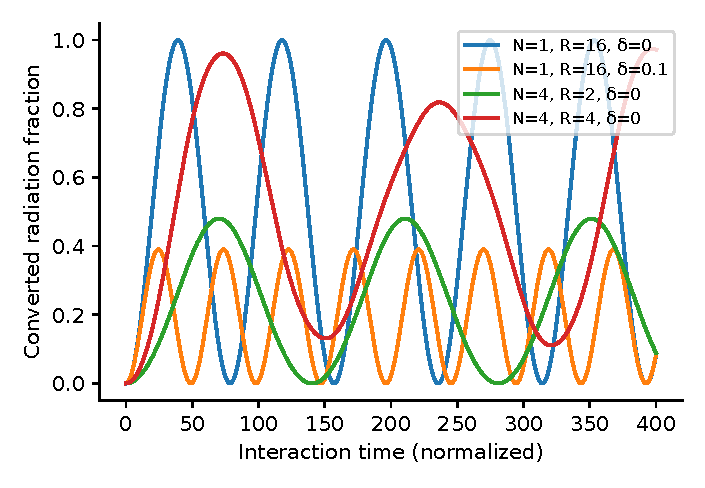
\includegraphics[width=0.9\textwidth,height=\textheight]{figures/review6_coherent_cells.pdf}
\caption{Finite-mode population evolution; reverse transitions and
capacity limits remain visible. The detuned single-packet example is not
an on-shell asymptotic scattering cross section.}
\end{figure}

Keeping \(Q\) fixed and choosing the on-resonance conversion duration
\(\pi/(2G)\) gives an energy-dependent detuning
\(\delta(E)=\sqrt{(\sqrt{E^2-m_A^2}-Q)^2+m_B^2}+\omega_b(Q)-E\). The
simulation uses 401 incident energies from 0.6 to 1.4. Away from the
matched energy, K10 yields different conversion probabilities. The final
free branch energy in this finite-time control need not equal
\(E-\omega_b\) when \(\delta\ne0\); the mismatch is explicitly stored,
not called an astronomical redshift. An actual spectral kernel must
enforce the full energy ledger including interaction/switching and
physical linewidth. Fixed-frequency mode conversion can be frequency
selective and cannot be extrapolated into an achromatic astronomical
aging law.

\begin{figure}
\centering
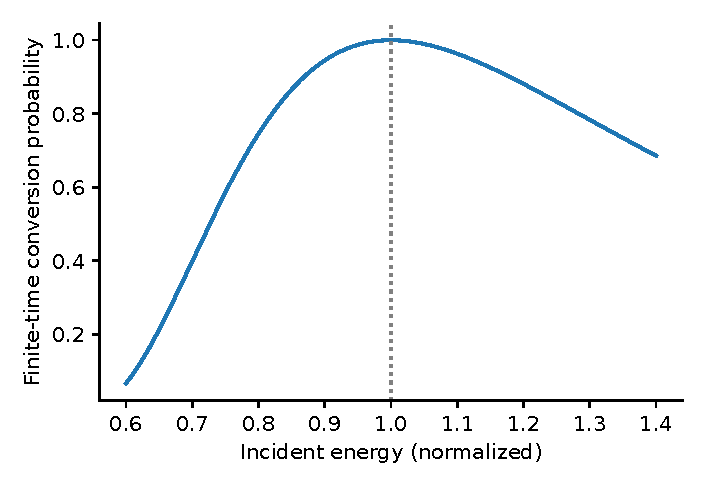
\includegraphics[width=0.9\textwidth,height=\textheight]{figures/review6_detuning.pdf}
\caption{Fixed phase-match mode and finite interaction duration:
incident-energy sensitivity of the converted population.}
\end{figure}

\subsection{Escape-assisted conversion: a continuous population
criterion}\label{escape-assisted-conversion-a-continuous-population-criterion}

The closed K9 cell does not supply a history law. A physical route to
approximate one-way transfer is emission into a reservoir mode that
transports energy and momentum away from the interaction region before
it can return. For a single resonant incident packet, take the
selected-mode coupling \(G>0\) and an outgoing escape channel with rate
\(\kappa\geq0\). The escaped state includes both the outgoing B packet
and the reservoir excitation outside the local interaction cell. In a
Markov approximation to a continuum with no incoming excitation, the
Lindblad jump is
\(\sqrt{\kappa}|B,\mathrm{escaped}\rangle\langle B,\mathrm{local}|\).
The no-jump amplitudes can be written as a real \(a\) and \(-i y\); the
escaped population is \(P_{\rm esc}\). Then

\[\begin{aligned}
\dot a&=-Gy,\quad \dot y=Ga-\frac\kappa2 y,\\
\dot P_{\rm esc}&=\kappa y^2,\\
a^2+y^2+P_{\rm esc}&=1.
\end{aligned}\tag{K11}\]

The escape term is not destruction of radiation or of reservoir energy:
it transfers the selected state out of the cell. The free ledger assigns
the same energy and momentum to the local and escaped B-plus-reservoir
states on resonance. A continuum dilation, outgoing boundary flux and
actual spectral density are required for a full local conservation
proof. A finite-temperature or reflected incoming reservoir requires the
reverse channel and its physical detailed balance; the vacuum
outgoing-boundary idealization is not valid in an arbitrary cosmic
environment. Rate \(\kappa\) is not derived here; a rough transport
timescale would involve the reservoir group speed and the physical
longitudinal interaction length, which must be computed rather than
fitted as a universal drag constant.

Eliminating \(y\) gives \(\ddot a+(\kappa/2)\dot a+G^2a=0\), with
\(a(0)=1\) and \(\dot a(0)=0\). For \(\kappa>4G\), put
\(\lambda=\sqrt{(\kappa/4)^2-G^2}\). The exact solution is

\[\begin{aligned}
a(T)&=e^{-\kappa T/4}\left[\cosh(\lambda T)+\frac{\kappa}{4\lambda}\sinh(\lambda T)\right],\\
y(T)&=\frac{G}{\lambda}e^{-\kappa T/4}\sinh(\lambda T).
\end{aligned}\tag{K12}\]

Both are nonnegative for all \(T\geq0\). At \(\kappa=4G\),
\(a=(1+GT)e^{-GT}\) and \(y=GT e^{-GT}\), also nonnegative. It follows
that

\[\kappa\geq4G\ \Longrightarrow\ \frac{d(1-a^2)}{dT}=2Gay\geq0.\tag{K13}\]

This is a continuous analytical monotonicity criterion for the
\emph{total converted population}, including escaped excitations. The
escaped population alone increases for every nonnegative escape rate.
For \(0\leq\kappa<4G\), the trigonometric continuation of K12 produces
oscillations and sign reversals of the total population derivative. Even
with no return of escaped states, coherent back-conversion occurs
locally before escape. In the very large escape-rate limit the
conversion becomes slow: the slow amplitude exponent approaches
\(-2G^2/\kappa\). Thus faster reservoir escape does not automatically
improve net conversion throughput.

Six escape ratios \(\kappa/G=0,1,2,4,8,16\) at \(G=0.04\) were compared
with a separate DOP853 solution of K11. The analytic and numerical
solutions agree to a maximum sampled absolute difference
\(1.54\,10^{-13}\) using relative tolerance \(10^{-12}\), absolute
tolerance \(10^{-14}\) and maximum step 1. The initial
unconstrained-step integration at the largest escape rate differed by
\(1.44\,10^{-8}\) and was refined; solver settings matter. First sampled
times for 90\% escape are respectively unavailable, 122, 59.5, 67, 118
and 231.5 in normalized time units. These are resolution-0.5
observations of the simulated curve; the continuous sign assertion
follows analytically from K12 rather than these samples.

\begin{figure}
\centering
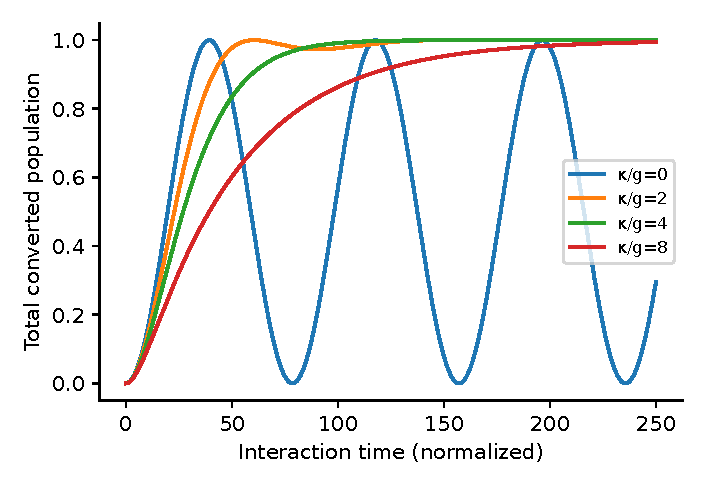
\includegraphics[width=0.9\textwidth,height=\textheight]{figures/review6_escape.pdf}
\caption{Escape-assisted converted-population control. At and above
critical damping the total converted population is monotonically
nondecreasing. Excessive escape slows net transfer.}
\end{figure}

Do not convert K13 into a single-photon speed theorem. A coherent
superposition has multiple dispersion poles and need not possess a group
velocity equal to its population-weighted branch speeds. Even for an
incoherent ensemble, a monotone mean speed is not a proof that every
packet continuously slows. The Part XXXI interval certificate concerns a
different, reduced trajectory and is retained without extension. A
physically derived multi-level dense dressing limit would have to give
an individual pole, a linewidth, a pathwise drift law and
energy/momentum/clock calibration, not merely monotonically changing
populations. K13 is useful because it identifies a concrete, testable
mechanism for suppressing local reverse conversion, not because it has
completed Foundation 3.

\subsection{Why static mixing and uniform temporal dressing are not the
history
law}\label{why-static-mixing-and-uniform-temporal-dressing-are-not-the-history-law}

For a single homogeneous branch \(E^2=C(T)^2p^2+\Delta(T)^2\),
translation invariance keeps \(p\) fixed. Differentiation gives

\[E\dot E=Cp^2\dot C+\Delta\dot\Delta.\tag{K14}\]

At fixed momentum, a growing gap with fixed or rising \(C\) cannot cause
an energy redshift. In a globally time-dependent regulator, energy can
fall despite growing gap only when \(Cp^2\dot C<-\Delta\dot\Delta\).
This is a condition on physical energy exchange with the regulator, not
a constitutive derivation. A static spatial variation conserves the
canonical energy for autonomous Hamiltonian evolution; real momentum
exchange and a recipient are required for cumulative spectral energy
change. As a counterfactual, imposing the Part XXXI reference final
energy 0.695302669585 and gap 0.5065013693 at the original fixed
momentum requires \(C_f=0.4763424873\), giving group speed 0.3263358177,
rather than the actual rising-wall exterior \(C_f=1.2\) and final speed
0.822104. A common temporal modulation is therefore not that reference
history mechanism. Keep C-01's environment-dependent regulator and
per-packet aging distinct until their reciprocal coupling is derived.

\subsection{Emission, detection, clocks and optical
timing}\label{emission-detection-clocks-and-optical-timing}

The C-01 exact initial ceiling is still a research requirement. From the
existing finite-gap dispersion, if an emission protocol is to be within
a fractional speed deficit \(\varepsilon\) of its local characteristic,
the exact condition is
\(\Delta/E\leq\sqrt{2\varepsilon-\varepsilon^2}\). It cannot yield exact
equality at finite positive gap. A phase-matched conversion is
downstream of emission and cannot repair this by redefining group speed
as wavefront speed. The numerical value of the regulator's local
characteristic must still be linked to dimensionless observations and a
measured source response.

Use conserved charged currents in J2, including physical atomic
transition matrix elements. If the receiver couples to the outgoing
branch with charge \(q_B\), its direct transverse amplitude contains
\(q_B\langle f|J_\perp|i\rangle e_B\). The squared coupling ratio
\(|q_B/q_A|^2\) is only a multiplicative comparison when the relevant
field normalizations and current matrix elements agree; a physically
normalized absorption rate also depends on the branch density of states,
recoil, spectral line and detector aperture. If \(q_B=0\) in an unmixed
reception region there is no direct absorption through that current.
Reconversion requires its own energy and momentum ledger. The positive
bare mass has not been reinterpreted as the ensemble-averaged gap. The
bound-state quantum receiver, longitudinal response beyond collinearity,
optical/nuclear rate response, and regulator backreaction are not yet
solved by K7--K13.

A stationary, one-dimensional reference with conversion at \(x=d\)
between fixed endpoints separated by one has actual path length one and
arrival time \(d/v_A+(1-d)/v_B\). For \(d=0.5\) the arrival time is
approximately 1.10285 rather than 1, while the equal-standard
transported spectral ratio is \(E_A/E_B=1.11731\). In a stationary
repeatable history, two identical pulses separated at emission have that
same interval at reception; the additional delay is not time stretching.
In a moving source/receiver or time-dependent environment, solve the
endpoint map rather than multiply the spectral ratio into the duration.
Use the clock-calibrated flux and distance relations of the preceding
sections. The receiver's local calibrated transition can change the
registered spectral ratio, and aperture losses change measured
brightness. The coherent direction control does not supply angular or
luminosity distances for actual galaxies; independent geometric anchors
and the physical three-dimensional matter flow remain required. No
arbitrary distance compression or claim of measured object size follows.

\subsection{Verification and next research
gates}\label{verification-and-next-research-gates}

The new numerical controls are supplied in
\nolinkurl{code/review6_forward.py} and
\nolinkurl{code/review6_escape.py}. They include 72 mediator rows, 15
finite-cell cases, 401 fixed-mode detunings, 8 aperture requirements,
and 6 analytic-versus-ODE escape cases. The first script records 137
regression assertions, including positivity, contact recovery, selected
refined quadratures, phase match and finite-cell unitarity and energy
tests; they are not experiments. The high-precision forward transfer and
log change of variable avoid subtracting nearly equal cosines at
arcsecond scales. Five selected quadratures were compared at tighter
relative tolerances, and the two Review 5.0 contact observables were
reproduced. Three extreme elastic rows triggered integration warnings
for small moment integrals (one selected refinement also warns); the
warning counts are retained and those rows are illustrative rather than
precision-certified. The central inelastic reference and selected
near-degenerate comparison do not have those warnings. Tree-level cross
sections are not nonperturbatively certified, and the coherent rate
\(G\) and escape rate \(\kappa\) are not calibrated. The original
21-case independent-audit benchmark and the earlier wall certificate are
preserved as source records; they are not represented as new independent
experiments or a newly executed interval proof in this edition.

Retain K1--K6 as a finite-range exchange candidate and its
large-transfer negative control. Retain K7--K10 as a phase-matched
selected-mode candidate and its finite-capacity, frequency and
reverse-transition controls. Retain K11--K13 as an analytical open-cell
population criterion under declared assumptions. None is identical to
Chapter 30S, Part XXXI or the Part XXXII contact conversion. A next
investigation must derive the actual material structure factor and
escape spectral density from a causal spatial reservoir, solve coupled
multimode dynamics including the detector current and thermal reverse
reactions, and establish whether the required forward momentum transfer
and linewidth can coexist. Extend pathwise monotonicity only with a
derived gap-history law and actual field backreaction. Then fit held-out
optical, timing, geometric-anchor and clock measurements with shared
parameters. Publication as an explicitly speculative research program
need not await that fit, but publication as a demonstrated replacement
for established cosmology would be unsupported.

\section{Observational discrimination and a unified-model
specification}\label{observational-discrimination-and-a-unified-model-specification}

\subsection{Measurement tests}\label{measurement-tests}

The model should be constructed from a local dynamical matter, field and
electromagnetic action or a precisely defined effective open-system
limit. It must specify physical source spectra, detector standards, a
causal initial-value problem, boundary conditions, conserved energy and
momentum including any bath, and enough independent measurements to
determine parameters. Recession and aging must not be tuned separately
for every source. A joint inference should use the same measured raw
observables and calibrated nuisance parameters for the ArcSecs candidate
and a conventional comparison model. Predeclare selection, systematics,
likelihoods and rejection criteria; do not rely on outliers discovered
after searching many datasets.

\begin{longtable}[]{@{}
  >{\raggedright\arraybackslash}p{(\columnwidth - 4\tabcolsep) * \real{0.3333}}
  >{\raggedright\arraybackslash}p{(\columnwidth - 4\tabcolsep) * \real{0.3333}}
  >{\raggedright\arraybackslash}p{(\columnwidth - 4\tabcolsep) * \real{0.3333}}@{}}
\toprule\noalign{}
\begin{minipage}[b]{\linewidth}\raggedright
Observable
\end{minipage} & \begin{minipage}[b]{\linewidth}\raggedright
Required model output
\end{minipage} & \begin{minipage}[b]{\linewidth}\raggedright
Decision criterion
\end{minipage} \\
\midrule\noalign{}
\endhead
\bottomrule\noalign{}
\endlastfoot
Atomic/nuclear clocks & Species-specific frequency ratios, motion and
environment & Reproduce laboratory and astrophysical precision
comparisons \\
Photon mass / radio dispersion & Longitudinal response, static range,
band-dependent group delays & Consistent with plasma-corrected and
laboratory limits in the specified mass mechanism \\
Geometric distances & Actual angular mapping, eclipsing-binary and
parallax inference & Recover independent anchors without redefining
distance units \\
Spectral redshift / SN timing & Moving endpoint spectra and broadband
light curves & Fit frequency shifts and observed arrival-time stretch
jointly \\
Flux / angular size & Forward and reverse beam maps, loss and emitted
luminosity & Fit \(D_L\), \(D_A\), and surface brightness using one
transport model \\
Redshift drift / structure & Evolution of recession and the
environmental field & Predict time dependence and clustering, not just a
static redshift law \\
Gravitation / multimessenger & Mode characteristics, lensing, clocks and
arrival lags & Reproduce measured constraints including GW170817 \\
Bubble search & Specified wall/exterior templates and predicted
correlations & Blinded held-out tests, trials-corrected significance,
null controls \\
\end{longtable}

GW170817/GRB 170817A places a differential speed constraint of roughly
\(-3\times10^{-15}\) to \(+7\times10^{-16}\) on gravitational versus
electromagnetic propagation in the published interpretation {[}6{]}.
This depends on emission-time and propagation assumptions. A common
environmental dependence can evade a \emph{differential} test, but must
be reconciled with clocks, matter and other modes. A photon-only
slowdown cannot simply ignore the comparison. The laboratory orientation
test of Nagel et al.~{[}7{]} likewise constrains anisotropic changes; it
does not directly bound an isotropic coordinate-speed parameter without
a matter and clock model. These established benchmarks should be used as
quantitative likelihood terms, not rhetorical endorsements of any
ontology.

\subsection{Minimum completion
criteria}\label{minimum-completion-criteria}

A unified candidate must simultaneously solve (i) cosmic mass
distribution and field response; (ii) actual inertial dynamics and
momentum transfer; (iii) positive-mass gauge and causal mode stability;
(iv) emission, aging and detection with consistent atomic standards; (v)
dynamical physical recession and lensing; (vi) 3D radiative transfer
with energy deposition; and (vii) observation-level distances, time
dilation and growth. Calibration must establish dimensionless
combinations from independent measurements rather than set the desired
answer. Strict emission at the ceiling, positive gap, and strict
universal age slowing form a central mathematical tension. Maintaining
all three requires a revised physical dispersion or nonlocal-history
mechanism with a causal local completion. The research should retain a
viable approximation if exact equality is not demonstrated, labeling the
departure from the charter requirement.

\subsection{Unified development and validation
sequence}\label{unified-development-and-validation-sequence}

The program now uses a versioned parameter ledger rather than
independent fitting knobs. Shared parameters are
\((C_*,\alpha,g,\lambda,C_I)\) for the regulator; positive invariant
mass and constitutive gap parameters for radiation; coupling and
capacity for the reservoir; matter response and domain boundary initial
data; gravitational coupling and mediator parameters; and independently
calibrated source/detector parameters. Each must have physical units, an
admissible range, an identified observation or derivation, and an
uncertainty. No numerical parameter set is selected by the present
review.

\begin{longtable}[]{@{}
  >{\raggedright\arraybackslash}p{(\columnwidth - 4\tabcolsep) * \real{0.3333}}
  >{\raggedright\arraybackslash}p{(\columnwidth - 4\tabcolsep) * \real{0.3333}}
  >{\raggedright\arraybackslash}p{(\columnwidth - 4\tabcolsep) * \real{0.3333}}@{}}
\toprule\noalign{}
\begin{minipage}[b]{\linewidth}\raggedright
Gate
\end{minipage} & \begin{minipage}[b]{\linewidth}\raggedright
Deliverable
\end{minipage} & \begin{minipage}[b]{\linewidth}\raggedright
Pass condition
\end{minipage} \\
\midrule\noalign{}
\endhead
\bottomrule\noalign{}
\endlastfoot
A: local dynamics & Action or explicit balance laws and characteristics
& Stable, causal, conserved energy and momentum; positive mass \\
B: C-01 & Finite 3D sources and clock/ruler response & Derive emission
ceiling; local and cosmic responses consistent \\
C: aging & Dynamic gap/history and bath solver & Nonincreasing speed
along paths; nonnegative reservoir energy; correct dispersion \\
D: emission and timing & Recoil, phase and packet arrival maps &
Atomic/nuclear standards, source motion, and timing all predicted \\
E: 3D optics & Forward/reverse ray bundles and radiative transfer &
Joint angle, flux, pulse and spectral prediction; anchor recovery \\
F: cosmology & Physical trajectories and likelihood & Shared parameters;
independent held-out distance and structure tests \\
G: boundaries & Dynamic wall and search templates & Predicted correlated
signals and trials-corrected validation \\
\end{longtable}

Retain failures in a compact mechanism decision ledger. Do not use them
to replace the owner-defined foundations, or discard observations that
constrain an implementation. The next numerical model should begin with
A--C in a dimensionless finite domain and add calibrated matter
standards before cosmological fitting. Compare against fixed-gap,
zero-drag, uniform-density and zero-coupling controls and report
resolution, conservation and boundary residuals. Use separate
calibration and validation data, with model comparison against
conventional estimators, not manually favorable distance ratios.

\section{Evidence and results ledger}\label{evidence-and-results-ledger}

\begin{longtable}[]{@{}
  >{\raggedright\arraybackslash}p{(\columnwidth - 4\tabcolsep) * \real{0.3333}}
  >{\raggedright\arraybackslash}p{(\columnwidth - 4\tabcolsep) * \real{0.3333}}
  >{\raggedright\arraybackslash}p{(\columnwidth - 4\tabcolsep) * \real{0.3333}}@{}}
\toprule\noalign{}
\begin{minipage}[b]{\linewidth}\raggedright
Source phase
\end{minipage} & \begin{minipage}[b]{\linewidth}\raggedright
Principal result
\end{minipage} & \begin{minipage}[b]{\linewidth}\raggedright
Scientific status
\end{minipage} \\
\midrule\noalign{}
\endhead
\bottomrule\noalign{}
\endlastfoot
Original reports / I--XI & Mass, clocks, relational gravity, distance,
bubble and dark-sector agenda; A-05c joint inconsistency & Premises,
proposed tests and restricted no-go \\
XII--XIV & Finite-size suppression weaker than local equilibrium
suggests; atomic drift and optical refraction & Conditional bounds and
illustrative numerical results \\
XV--XVII & Recession + slowing distance law; singularity then bounded
model; high-\(z\) size and drift tension & Derived candidate failures \\
XVIII--XX & Conservative mode coupling; Stueckelberg/Yukawa sector;
atomic shifts & Restricted analytical and numerical demonstrations \\
XXI--XXII & Autonomous 1D separation and moving atomic endpoints &
Dimensionless toy; motion dominates selected spectra \\
XXIII--XXIV & Packet reach differs from causal reach; bounded scalar
energy prevents eternal zero speed & Conditional mathematical
reachability and energy bound \\
XXV & 2D autonomous clumps; competing scalar attraction and repulsion;
planar refraction & Numerical toy, no physical calibration \\
XXVI & Reciprocal optical maps; weak spherical defocusing; brightness
factor tension & 3D static/axisymmetric audit, no fitted cosmology \\
XXVII & C-01 mass-sourced regulator and shell/void tests & Candidate
wave-speed law; fails monotone aging across shell \\
XXVIII & Passive fixed-gap drag; tiny speed change at modest redshift;
stationary pulse stretching absent & Exact restricted benchmark +
executed quadrature checks \\
XXIX & Six-report and four-explorer curation; corrected phase/group and
timing formulas; impedance matching and material-flow interfaces &
Source-grounded synthesis; reported explorer simulations not
reproduced \\
XXX & Exact fixed-gap wall energy bound and linear-wall drag feasibility
inequality; 28 automated calculation checks & Conditional analytical and
numerical results \\
XXXI & Positive-gap conversion with finite recoil and heat ledger;
finite-capacity bound; 42 historical runs and 135 automated assertions &
Conditional packet benchmark; no microscopic or observational
completion \\
XXXII / Review 4.0 & Bounded flow, calibration, wall recoil, reversible
local conversion and directional optics & Executed reduced controls; no
unified physical or observational fit \\
XXXIII / Review 5.0 & Bounded action, differential scattering,
reversible cell and static-wall interval certificate & Conditional
mathematical and numerical results; strong scattering in reference
channel; no microscopic or observational closure \\
XXXIV / Review 6.0 & Finite-range transfer floor; collinear phase match;
escape criterion & Conditional local controls; no derived cosmic
coherence or individual history \\
\end{longtable}

No row constitutes a confirmed measurement of nonzero photon rest mass,
a discovery of a cosmic wall, a measured change of the vacuum
light-speed ceiling, or a demonstrated overestimate of all astronomical
distances. A failed implementation is preserved as a result; future
mechanisms should not reintroduce the same failure in new notation
without addressing it.

\section{Discussion and conclusion}\label{discussion-and-conclusion}

ArcSecs now has an integrated research architecture rather than six
independent explanatory narratives. Its principal question is C-01:
whether the local emission ceiling can arise from the physical
distribution of cosmic matter and its collective inertial response. A
retarded regulator with impedance-matched electromagnetic constitutive
coefficients offers a defined route to investigate that possibility. A
positive regulator amplitude within a hollow cavity is mathematically
compatible with zero ordinary Newtonian shell force; this does not
establish the existence of a wall or derive the observed speed ceiling.
A material flow on fixed coordinates supplies a precise
physical-recession research direction, while the operational clock and
ray endpoint maps distinguish spectral redshift from measured temporal
stretching.

The new Part XXX calculation strengthens the wall-crossing requirement:
a tiny fixed gap makes passive drag inefficient at reducing speed, and
monotone crossing into a larger characteristic speed demands a severe
energy loss. Constant drag strong enough to satisfy monotonicity in the
illustrative wall stops the packet inside it. A dynamic gap or causal
history field must therefore be derived and account for energy, recoil,
dispersion and detector response. These results narrow the permissible
implementations of the proposed aging mechanism without assuming a
favorable empirical outcome. The one-megaparsec example demonstrates a
travel-time inference bias; it is not a proof that angular or luminosity
distances are overestimated. Any reduction of apparent extreme-object
sizes must follow from an anchor-calibrated optical and timing model.

Part XXXI demonstrates that an additional history coordinate can evade
the fixed-gap endpoint restriction in a selected reduced wall model
while maintaining explicit recoil, heat and wall-reaction ledgers. Its
finite-capacity bound and strong emission-energy dependence prevent
interpreting that example as a universal solution. Review 4.0 adds a
bounded matter-flow control, calibrated brightness relation, finite wall
recoil and a local reversible gauge-invariant branch-conversion
candidate. These are not yet one theory. Review 5.0 adds a bounded
classical action, exact differential scattering and a finite-capacity
reverse-reaction control; the selected contact interaction fails
narrow-beam transport, and continuous monotonicity is now certified by
interval comparison only for the original static smooth-wall reference.
Review 6.0 adds a finite-range exchange obstruction, a collinear
phase-matched conversion, a reciprocal finite-cell benchmark and an
analytic escape-assisted population criterion. A derived spatial
reservoir, single-packet history, physical emission mechanism and
conserved-current detector with atomic/nuclear calibration, coupled to
autonomous matter and regulator dynamics, remain the next priority.
Derive rather than stipulate the one-way conversion law. Advance the six
branches together through the validation gates, not by adding unrelated
fitted effects. The twelve foundations and C-01 clarification remain the
research charter; no complete observationally successful implementation
is yet demonstrated. The revised paper is intended for review,
correction and continued constructive mathematical development.

\section{References and source
lineage}\label{references-and-source-lineage}

The following selected literature records are carried forward from the
preceding reviews. They are not represented as newly independently
verified in Review 6.0. They support the specified benchmark or
historical point, not the ArcSecs conclusions as a whole. Additional
references and their original context are contained in each archived
manuscript.

\begin{enumerate}
\def\labelenumi{\arabic{enumi}.}
\tightlist
\item
  Sciama, D. W. (1953). On the Origin of Inertia. \emph{Monthly Notices
  of the Royal Astronomical Society}, 113, 34--42.
  \url{https://doi.org/10.1093/mnras/113.1.34}.
\item
  Tu, L.-C., Luo, J., \& Gillies, G. T. (2005). The mass of the photon.
  \emph{Reports on Progress in Physics}, 68, 77--130.
  \url{https://doi.org/10.1088/0034-4885/68/1/R02}.
\item
  Adelberger, E., Dvali, G., \& Gruzinov, A. (2007). Photon-mass bound
  destroyed by vortices. \emph{Physical Review Letters}, 98, 010402.
  \url{https://pubmed.ncbi.nlm.nih.gov/17358459/}.
\item
  Pietrzyński, G., et al.~(2019). A distance to the Large Magellanic
  Cloud that is precise to one per cent. \emph{Nature}, 567, 200--203.
  \url{https://doi.org/10.1038/s41586-019-0999-4}.
\item
  Dark Energy Survey Collaboration (2024). The Dark Energy Survey
  Supernova Program: slow supernovae show cosmological time dilation out
  to z \textasciitilde{} 1. \emph{MNRAS}, 533, 3365.
  \url{https://arxiv.org/abs/2406.05050}.
\item
  Abbott, B. P., et al.~(2017). Gravitational Waves and Gamma-Rays from
  a Binary Neutron Star Merger: GW170817 and GRB 170817A.
  \url{https://arxiv.org/abs/1710.05834}.
\item
  Nagel, M., et al.~(2015). Direct terrestrial test of Lorentz symmetry
  in electrodynamics to \(10^{-18}\). \emph{Nature Communications}, 6,
  8174. \url{https://doi.org/10.1038/ncomms9174}. Carried forward from
  Part XXVII's literature review.
\end{enumerate}

\textbf{Internal source references.} {[}A1{]}
\nolinkurl{Deriving the Screened Common-Field Model(1).md} (Part IX).
{[}A2{]} original archive
\nolinkurl{09_Bubble_Observational_Tests_Full_Depth.zip} and 15
standalone reports (register IDs L01--L15 and Z01--Z23). {[}A3{]}
\nolinkurl{ArcSecs_Part_XII_Research.md} through
\nolinkurl{ArcSecs_Part_XXVII_Research.md} (available installments).
{[}A4{]} C-01 integrated addendum and \texttt{.uai} high-priority
research notes. {[}A5{]} Part XXVIII calculations,
\nolinkurl{code/photon_aging.py}, with CSV and verification log. The
earlier full review archive contains these source materials and
available earlier numerical packages; this update contains the active
curated sources and new benchmarks. Original report citations are
retained as recorded; this review does not independently audit every
historical claim or source.

\subsection{Review 5.0 additional source
checks}\label{review-5.0-additional-source-checks}

\begin{itemize}
\tightlist
\item
  Particle Data Group, \emph{Kinematics}, 2021 review, two-body
  scattering normalization:
  \url{https://pdg.lbl.gov/2021/reviews/rpp2021-rev-kinematics.pdf}.
  Used for J10 phase-space convention; matrix element derived here from
  H3/J1.
\item
  Pietrzyński et al.~(2019), \emph{A distance to the Large Magellanic
  Cloud that is precise to one per cent}, Nature 567, 200--203.
  \url{https://doi.org/10.1038/s41586-019-0999-4}. Anchor value and
  uncertainties.
\item
  Reid, Pesce and Riess (2019), \emph{An Improved Distance to NGC 4258
  and Its Implications for the Hubble Constant},
  \url{https://arxiv.org/abs/1908.05625}. Anchor distance and quoted
  statistical/systematic errors; no raw-observable refit.
\item
  Independent ArcSecs audit archive (supplied 24 November 2026),
  correction ledger SCI-001 and PUB-003 and independent numerical
  implementation. Original ZIP and selected extracted sources in
  historical/independent\_audit; see source hashes and comparison log.
  Audit coverage was targeted, not a complete verification of the entire
  book.
\end{itemize}

\subsection{Review 6.0 source and provenance
additions}\label{review-6.0-source-and-provenance-additions}

\begin{itemize}
\tightlist
\item
  Particle Data Group, \emph{Kinematics and Cross-Section Formulae},
  2025 index:
  \url{https://pdg.lbl.gov/2025/reviews/kinematics_and_cross_sections.html}.
  Phase-space convention inherited from J10; K4--K13 are derived
  controls in this manuscript.
\item
  \emph{Photon-dark photon conversion with multiple level crossings},
  Phys. Rev.~D 108, 095045 (2023),
  \url{https://doi.org/10.1103/PhysRevD.108.095045}. Related literature
  lead for coherent mode conversion, not support for the specific
  ArcSecs reservoir or a verified cosmology.
\item
  Current supplied hardcover, independent-audit integration edition with
  Review 5.0 (24 November 2026). SHA-256, text concordance and geometry
  results in the Review 6.0 book preflight. The 109-page protected
  manuscript matched the standalone text after exclusion of its added
  book footer.
\end{itemize}

\section{Reproducibility, provenance and publication
notes}\label{reproducibility-provenance-and-publication-notes}

The independent source title is unchanged; Review 3.0, Review 4.0 and
Review 5.0 source and PDF are preserved byte-for-byte under
\nolinkurl{historical/}. Page 10 of the supplied book is the
authoritative charter source. The earlier edition's pages 119--122
(Galilean control), 126 and 137 (tidal sign), 258--267 (scalar bath),
and 340--380 (Review 3.0) are historical references. In the revised
hardcover, the corresponding main-book controls begin at pages 120, 128
and 139, and 260; the protected Review 4.0 section begins at page 343.
The latest supplied Review 5.0 hardcover has 456 physical pages, with
the standalone review on pages 347--455. These are distinct from the
historical Review 4.0 locations. The book's main text has not been
edited here. The independent audit's supplied PDF matches the revised
book byte-for-byte. It counted 430 physical pages; the numbered text
ends at 429. The earlier archive and curated reports supply historical
research lineage; older results not rerun in Review 4.0 are identified
as inherited. See the reference/provenance register and revision log for
source locations and status.

From the archive root, run \texttt{python}
\nolinkurl{code/review4_benchmarks.py}, \texttt{python}
\nolinkurl{code/review4_recoil_optics.py} and \texttt{python}
\nolinkurl{code/review4_extra_controls.py}. The first creates the
fixed-wall extrema, status, flow, collision, clock and occupancy
datasets and three vector plots. The second creates the recoil and
optical Jacobi datasets and one vector plot. The third verifies the
analytical bounded-flow derivative, clock/unit conversion, the charter
transcription and energy/momentum/optical arithmetic. The exact
parameter values are included in each script and output CSV, and the
dependencies in \nolinkurl{appendices/review4_dependencies.txt}.
Recorded solver tolerances, threshold events and accepted step counts
appear in the wall CSV. Automated assertions are regression tests of
specific calculations, not independent physical experiments. Solver
convergence and residuals are not validated interval bounds. The
historical Part XXVIII, XXX and XXXI scripts and datasets remain
available without modification. Their complete source and data are not
to be mistaken for a published observational likelihood.

Review 5.0 adds \nolinkurl{code/review5_microscopic.py} and
\nolinkurl{code/review5_interval_wall.py}. Run each with Python from the
archive root. The first writes differential integrated cross sections,
source recoil, pole, kinetic-cell, aperture and anchor controls with 277
regression assertions; 201 of these are individual positivity grid
checks, not independent experiments. The second writes interval
enclosure and certificate records at coarse and fine position steps (run
with \texttt{-\/-steps\ 1000} and \texttt{-\/-steps\ 2000}). The
independent audit implementation is preserved and rerun in
\nolinkurl{appendices/audit_regression/}; compare its outputs against
the archived audit data. Use the supplied comparison and source hashes;
no claim of observational validation follows from exact code
reproduction.

Review 6.0 adds \nolinkurl{code/review6_forward.py} and
\nolinkurl{code/review6_escape.py}. The outputs and dependency versions
are in the new CSV, JSON and execution logs. Earlier results are
inherited unless specifically rerun; the independent audit record and
Review 5.0 source remain unchanged in the historical archive. The new
chapter records quadrature warnings and limits.

\par

Build with \nolinkurl{bash code/build_review6.sh}. Markdown and LaTeX
sources are provided. All printed figures are vector; historical raster
figures remain in the archive. Trim is 6.14 by 9.21 inches, no bleed,
0.75-inch inner and 0.65-inch outer mirrored margins, embedded fonts and
11-point body. Reassess combined book pagination, parity, gutter and
cover. No KDP upload or physical proof was performed. SHA-256 verifies
bytes, not scientific validity. Portable \texttt{.uai} records preserve
decisions; no remote repository was changed.

\end{document}
